% $Id: INF_Diplomarbeit.tex 1660 2010-02-25 13:57:42Z tkren $
%
% TU Wien - Faculty of Informatics
% thesis template
%
% This template is using the memoir document class, see
% <http://www.ctan.org/tex-archive/macros/latex/contrib/memoir/memman.pdf>
% <http://www.ctan.org/info/latex-samples/MemoirChapStyles/MemoirChapStyles.pdf>
% 
% For questions and comments send an email to
% Thomas Krennwallner <tkren@kr.tuwien.ac.at>
%

								
\documentclass[a4paper,12pt, oneside]{memoir}
%\chapterstyle{veelo}
\usepackage{graphicx} 
\usepackage{placeins}
\usepackage{caption}


\chapterstyle{madsen}
\setlength{\parskip}{6pt plus 1pt minus 1pt}
\setlength{\parindent}{0pt}

\usepackage{TUINFDA}

\thesistitle{Geocluster: Server-side clustering in Drupal based on Geohash}
\thesisdate{\the\day.\the\month.\the\year}

\thesisdegree{Diplom-Ingenieur}
\thesiscurriculum{Software Engineering and Internet Computing}
\thesisverfassung{Verfasser}
\thesisauthor{Josef Dabernig}
\thesismatrikelno{0927232}
% \thesisauthoraddress{} % your address

\thesisbetreuung{Betreuer}
\thesisbetreins{Prof.~Dr.~A Min Tjoa}
\thesisbetrzwei{Univ.-Ass.~Dr. Amin Anjomshoaa}

\newcommand{\EnableCustomThesisLayout}{
\setheaderspaces{*}{1.5cm}{*}
}

\usepackage{multirow}
\usepackage{rotating}

\begin{document}


% the front matter                                                 
\frontmatter

% $Id: titlepage.tex 2165 2010-08-07 04:42:52Z tkren $
%
% TU Wien - Faculty of Informatics
% thesis titlepage
%
% This titlepage is using the geometry package, see
% <http://www.ctan.org/macros/latex/contrib/geometry/geometry.pdf>
%
% For questions and comments send an email to
% Thomas Krennwallner <tkren@kr.tuwien.ac.at>
%

% setup page dimensions for titlepage
\newgeometry{left=2.4cm,right=2.4cm,bottom=2.5cm,top=2cm}

% force baselineskip and parindent
\newlength{\tmpbaselineskip}
\setlength{\tmpbaselineskip}{\baselineskip}
\setlength{\baselineskip}{13.6pt}
\newlength{\tmpparindent}
\setlength{\tmpparindent}{\parindent}
\setlength{\parindent}{17pt}
\newlength{\tmpparskip}
\setlength{\tmpparskip}{\parskip}
\setlength{\parskip}{0pt}


% first titlepage
\thispagestyle{tuinftitlepage}

%
% Kludge: for each titlepage set \pagenumbering to a different
% style. This is used to fix a problem with hyperref, because there
% are multiple "page 1" and hyperref hates that
%
\pagenumbering{Alph}

\begin{center}
%
\begin{minipage}[t][5.2cm][b]{\linewidth}%
    \centering%
    %\renewcommand{\baselinestretch}{0.9} % very long titles need to tweak baselinestretch...
    \thesistitlefontHUGE\sffamily\bfseries\tuinfthesistitle%
\end{minipage}


\vspace{1.3cm}

{\thesistitlefontLARGE\sffamily \tuinfthesistype}

\vspace{6mm}

{\thesistitlefontlarge\sffamily zur Erlangung des akademischen Grades}

\vspace{6mm}

{\thesistitlefontLARGE\sffamily\bfseries \tuinfthesisdegree}

\vspace{6mm}

{\thesistitlefontlarge\sffamily im Rahmen des Studiums}

\vspace{6mm}

{\thesistitlefontLarge\sffamily\bfseries \tuinfthesiscurriculum}

\vspace{6.5mm}

{\thesistitlefontlarge\sffamily eingereicht von}

\vspace{6mm}

{\thesistitlefontLarge\sffamily\bfseries \tuinfthesisauthor}

\vspace{1.5mm}

{\thesistitlefontlarge\sffamily Matrikelnummer \tuinfthesismatrikelno} 

\vspace{1.5cm}

\begin{minipage}[t][1.7cm][t]{\textwidth}%
  \vspace{0pt}\raggedright\thesistitlefontnormalsize\sffamily
  %
  an der

  Fakult\"{a}t f\"{u}r Informatik der Technischen Universit\"{a}t Wien
\end{minipage}

\begin{minipage}[t][4cm][t]{\textwidth}%
  \vspace{0pt}\sffamily\thesistitlefontnormalsize\raggedright
  %
  Betreuung

  \tuinfthesisbetreuung: \tuinfthesisbetreins

  \raggedright Mitwirkung: \tuinfthesisbetrzwei

\end{minipage}

% we want a german date, then switch back to english
\selectlanguage{ngerman}
\begin{minipage}[t][2cm][t]{\textwidth}%
  \vspace{0pt}\sffamily\thesistitlefontnormalsize
  \begin{tabbing}%
    \hspace{42mm} \= \hspace{66mm} \= \hspace{51mm} \kill
    Wien, \tuinfthesisdate \> {\raggedright\rule{51mm}{0.5pt}} \> {\raggedright\rule{51mm}{0.5pt}} \\
    \> \begin{minipage}[t][0.5cm][t]{51mm}\centering (Unterschrift \tuinfthesisverfassung)\end{minipage}
    \> \begin{minipage}[t][0.5cm][t]{51mm}\centering (Unterschrift \tuinfthesisbetreuung)\end{minipage}
    \end{tabbing}
\end{minipage}
\selectlanguage{english}

\end{center}

% we want an empty page right after first titlepage
\cleardoublepage

% we're done with the titlepages, proceed with default pagenumbering
\pagenumbering{roman}

% restore baselineskip
\setlength{\baselineskip}{\tmpbaselineskip}
\setlength{\parindent}{\tmpparindent}
\setlength{\parskip}{\tmpparskip}


% back to normal geometry
\restoregeometry


%%% Local Variables:
%%% TeX-PDF-mode: t
%%% TeX-debug-bad-boxes: t
%%% TeX-parse-self: t
%%% TeX-auto-save: t
%%% reftex-plug-into-AUCTeX: t
%%% End:

\EnableCustomThesisLayout
\chapter*{Erklärung zur Verfassung der Arbeit}

\tuinfthesisauthor\\
% \tuinfthesisauthoraddress

\vspace*{1.2cm}

Hiermit erkläre ich, dass ich diese Arbeit selbständig verfasst habe, 
dass ich die verwendeten Quellen und Hilfsmittel vollständig angegeben 
habe und dass ich die Stellen der Arbeit - einschließlich Tabellen, 
Karten und Abbildungen -, die anderen Werken oder dem Internet im 
Wortlaut oder dem Sinn nach entnommen sind, auf jeden Fall unter Angabe 
der Quelle als Entlehnung kenntlich gemacht habe.\\



  \begin{tabbing}%
    \hspace{15mm} \= \hspace{65mm} \= \hspace{42mm} \kill
    \> Wien, \tuinfthesisdate \> {\raggedright\rule{51mm}{0.5pt}} \\
    \> \> \begin{minipage}[t][0.5cm][t]{51mm}\centering
 (Unterschrift \tuinfthesisverfassung)\end{minipage}
  \end{tabbing}


%
% abstract
%


\chapter*{Abstract}

This thesis investigates the possibility of creating a server-side clustering solution for mapping in Drupal based on Geohash. Maps visualize data in an intuitive way. Performance and readability of digital mapping applications decreases when displaying large amounts of data. Client-side clustering uses JavaScript to group overlapping items but server-side clustering is needed when too many items slow down processing and create network bottle necks. The main goals are: implement real-time, server-side clustering for up to 1,000,000 items within 1 second and visualize clusters on an interactive map.

Clustering is the task of grouping unlabeled data in an automated way. Algorithms from cluster analysis are researched in order to create an algorithm for server-side clustering with maps. The proposed algorithm uses Geohash for creating a hierarchical spatial index that supports the clustering process. Geohash is a latitude/longitude geocode system based on the Morton order. Coordinates are encoded as string identifiers with a hierarchical spatial structure. The use of a Geohash-based index allows to significantly reduce the time complexity of the real-time clustering process.

Three implementations of the clustering algorithm are realized as the Geocluster module for the free and open source content management system and framework Drupal. The first algorithm implementation based on PHP, Drupal's scripting language, doesn't scale well. A second MySQL-based clustering has been tested to scale up to 100,000 items within one second. Finally, clustering using Apache Solr scales beyond 1,000,000 items and satisfies the main research goal of the thesis.

In addition to performance considerations, visualization techniques for putting clusters on a map are researched and evaluated in an exploratory analysis. Map types as well as cluster visualization techniques are presented. The evaluation classifies the stated techniques for cluster visualization on maps and provides a foundation for evaluating the visual aspects of the Geocluster implementation.

\newpage

% and in German
\chapter*{Kurzfassung}

Diese Diplomarbeit erforscht die technische M\"{o}glichkeit zur Erstellung einer Geohash-basierten, server-seitigen Cluster-L\"{o}sung f\"{u}r Kartenanwendungen in Drupal. Landkarten visualisieren Daten auf intuitive Weise. Die Performanz und Lesbarkeit von digitalen Kartenanwendungen nimmt jedoch ab, wenn umfangreiche Datenmengen dargestellt werden. Mittels JavaScript gruppiert Client-seitiges Clustering \"{u}berlappende Punkte zwecks Lesbarkeit, ab einer gewissen Datenmenge verlangsamt sich jedoch die Verarbeitungsgeschwindigkeit und die \"{u}bertragungsgeschwindigkeit des Netzwerk stellt einen Flaschenhals dar. Die zentrale Forschungsfrage ist daher: Implementierung von server-seitigem Clustering in Echtzeit f\"{u}r bis zu 1.000.000 Punkten innerhalb einer Sekunde und die Visualisierung von Clustern auf einer interaktiven Karte.

Clustering ist ein Verfahren zur automatisierten Gruppierung in Datenbest\"{a}nden. Algorithmen der Clusteranalyse werden evaluiert, um einen geeigneten Algorithmus f\"{u}r das server-seitige Clustering auf Landkarten zu schaffen. Der entworfene Algorithmus nutzt Geohash zur Erstellung eines hierarchischen, Spatialindex welcher das Clustern unterst\"{u}tzt. Geohash ist kodiert Latitude/Longitude Koordinaten mithilfe der Morton-Kurve in Zeichenketten mit r\"{a}umlich-hierarchischer Struktur. Mithilfe eines Geohash-basierten Index kann die Zeitkomplexit\"{a}t des Echtzeit-Clusterings drastisch reduziert werden.

3 Varianten des Clustering Algorithmus wurden als Geocluster Modul f\"{u}r das Content Management System und Framework Drupal implementiert. Die erste, PHP-basierte Variante skaliert nicht. Die zweite Variante mittels MySQL konnte in Tests bis 100.000 Punkte unter 1 Sekunde clustern. Schlussendlich skaliert das Clustern mit Apache Solr bis \"{u}ber 1.000.000 Elemente und erf\"{u}llt somit das prim\"{a}re Forschungsziel.

Neben der Performance-Analyse wurden auch Techniken zur Visualisierung von Clustern auf Karten erforscht und im Rahmen einer explorativen Studie verglichen. Verschiedene Kartentypen als auch Visualisierungsformen von Clustern werden pr\"{a}sentiert. Die Evaluierung klassifiziert die Techniken zwecks der Darstellung auf Karten und bildet somit die Grundlage f\"{u}r die Diskussion der Geocluster Implementierung.  
\newpage

\setcounter{tocdepth}{3}
\tableofcontents
\newpage

%TODO enable
%\listoffigures
\newpage

%\listoftables
\newpage

%
% start of the thesis
%
\mainmatter
\setcounter{secnumdepth}{3}


%
% intro
%

\chapter{Introduction}


\section{Motivation}

Digital mapping applications on the Internet are strongly emerging. Big players like Google Maps\footnote{\url{https://maps.google.at}} and OpenStreetMap\footnote{\url{http://www.openstreetmap.org/ }} provide online maps, that users can view and interact with. 

Maps allow telling stories and communicating data in a visual way. Using open source tools such as TileMill\footnote{\url{http://mapbox.com/tilemill}} and online services like CloudMade\footnote{\url{http://cloudmade.com/ }}, more and more people are able to create their own custom maps. The Free and Open Source content management system and framework Drupal\footnote{\url{http://drupal.org}} provides tools for adding, editing and visualizing geographic data on maps. This allows to integrate interactive map applications into web sites.

Maps provide a birds-eye-view on the geography and information captured in such system. Sometimes, they are used to get a quick overview of points-of-interest in a certain area. If a large amount of information is contained in such an area, problems in terms of computability and visual clutter arise: visualizing thousands of points on a single map both challenge human and computers. Obviously, when telling a story, information needs to be told in a compact way as the human brain can only process a limited amount of data at the same time. Similarly, large amounts of data involve a higher burden on the computer components that participate in the web mapping process~~\cite{noellenburg11geovis, Delort10vis}.

Clustering\footnote{\url{http://en.wikipedia.org/wiki/Cluster_analysis}} is a technique for grouping objects with similarities that can be used to reduce visual clutter as described before. Various client-side Javascript libraries like Leaflet.markercluster\footnote{\url{https://github.com/Leaflet/Leaflet.markercluster}} exist for clustering points on maps. This enhances performance and readability of data-heavy map applications. But still, all data needs to be transferred to the client and processed on a potentially slower end user device. By clustering data on the server-side, the load is shifted from the client to the server which allows displaying larger amounts of data in a performant way. Professional services like maptimize\footnote{\url{http://www.maptimize.com}} provide such a functionality, while in the open source space little libraries and frameworks exist for server-side clustering of geospatial data.

In order to create interactive maps based on large data sets, this thesis evaluates and implements a performance-optimized server-side clustering algorithm for Drupal.


\section{Outline of the thesis}

Chapter \ref{chapter:foundations} introduces the technical foundations for this thesis. It provides an overview by explaining cluster theory and comparing four main clustering algorithms. Further, a discussion on spatial data computation introduces space order and space decomposition methods, Quadtrees and the Geohash encoding. An overview of foundational concepts in web mapping as coordinate systems, map projections and spatial data types is provided. Finally, basic concepts of geovisualization as visual variables, visual data exploration techniques and clutter reduction are explained. 

Chapter \ref{chapter:state} discusses the state of the art of related technologies for the thesis. An explanation of a modern web mapping stack is given as well as the basics of Drupal \& mapping technologies. Further, the state of the art for client-side and server-side clustering technologies in web mapping is analyzed. The chapter is concluded by a section on visual mapping that list map visualization types, as well as cluster visualization techniques and summarizes them in an evaluation. 

Chapter \ref{chapter:objectives} states the objectives and exemplary use cases for the thesis. It defines the goals to be accomplished as a result of the implementation part of the thesis.

Chapter \ref{chapter:realization} describes the realization of the server-side clustering algorithm. First, an analysis based on the objectives stated in the previous chapter is given. Subsequently, the Geohash-based clustering algorithm is defined. Finally, the architecture and implementation of the algorithm for Drupal is explained in detail.

Chapter \ref{chapter:use-cases} discusses the implementation of use cases for the realized server-side clustering algorithm.

Chapter \ref{chapter:conclusions-outlook} finally evaluates the results of the thesis. It contains performance tests and a visual evaluation on how the defined objectives have been accomplished. Final conclusions are made and an outlook on future work is given.






%
% foundations
%

\chapter{Foundations}
\label{chapter:foundations}

TODO: introduction


%
% foundations - clustering
%

\section{Clustering}

Clustering is the task of grouping unlabeled data in an automated way. It can also be described as the unsupervised classification of patterns into groups. The techniques of cluster analysis are applied in numerous scenarios including data mining, document retrieval, image segmentation and pattern classification. They are used to solve different tasks including pattern-analysis, grouping, decision-making or machine-learning.

Cluster analysis has been studied since the early beginnings of computer science and applies to a broad number of research fields. Different research communities have created a variety of vocabularies to describe methods related to clustering. Analog to the term cluster analysis, other names are used in literature: Q-analysis, topology, grouping, comping, classification, numerical taxonomy and unsupervised pattern recognition.

As indicated, clustering is a wide and generic term. Often it is used to refer to specific concepts which are appropriate for solving specific tasks. This means that efficient clustering algorithms have been developed and studied over the years for certain research fields. While such algorithms might perform well under certain circumstances, they might be completely inappropriate for other use cases. Imagine, an algorithm that  fits image segmentation well but is less useful in machine-learning~\cite{Meert06clustermaps, Jain99clusterreview}.

Clustering is a general concept that applies to multivariate data. Spatial data in this sense is a special case, and 2-dimensional spatial data reduces the problem space even further to planar space. Figure~\ref{fig:clusters} visualizes such an example of clusters of point patterns in two dimensional space. Humans can understand and perform this kind of clustering tasks competitively whereas clustering in high-dimensional space is difficult for humans to obtain. 

\begin{figure}[h]
  \begin{center}
    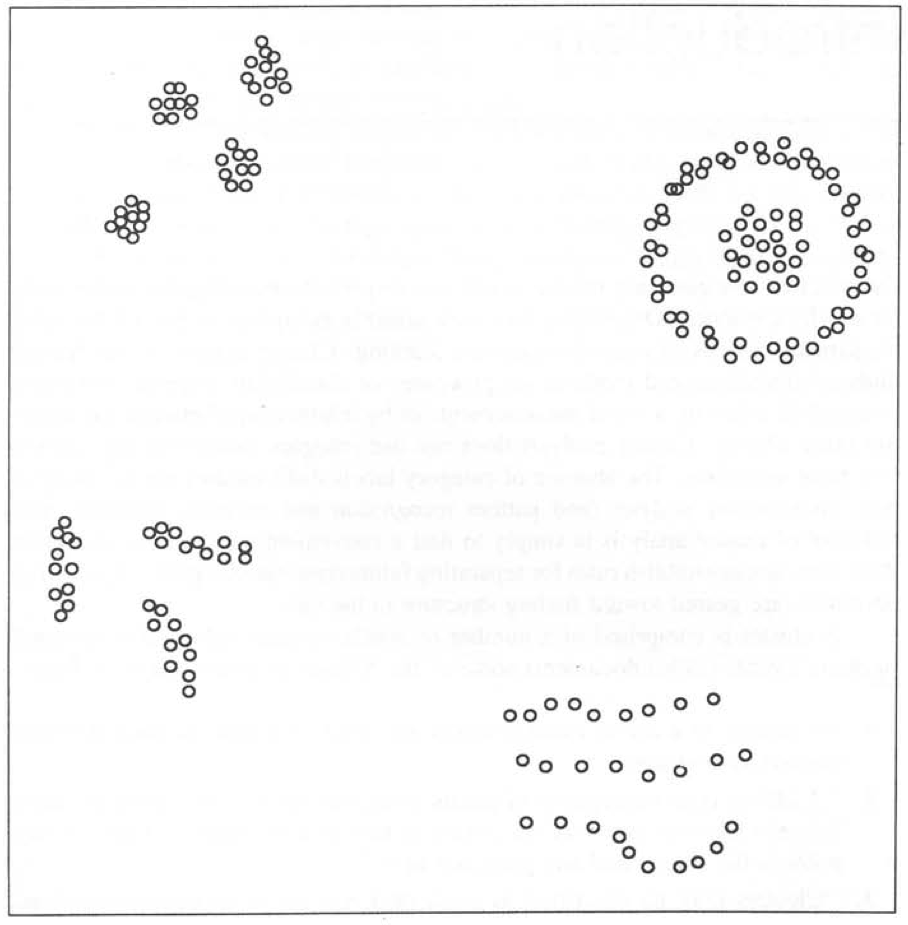
\includegraphics[width=0.75\textwidth]{figures/clusters.png}
    \caption{Clusters of point patterns in two dimensions~\cite[p 2]{Jain99clusterreview}.}
    \label{fig:clusters}
  \end{center}
\end{figure}



\subsection{The Clustering task}

Clustering is the task of aggregating items (also described as features) into clusters, based on similarities or proximity. A.K. Jain, M.N. Murty and P.J. Flynn~\cite{Jain99clusterreview} define the following steps involved in a typical pattern clustering activity:
 
\begin{quote}
\begin{enumerate}
\item pattern representation (optionally including feature extraction and/or selection), 
\item definition of a pattern proximity measure appropriate to the data domain, 
\item clustering or grouping, 
\item data abstraction (if needed), and 
\item assessment of output (if needed). 
\end{enumerate}
\end{quote}



\subsection{History}

K-means, one of the oldest and most widely used clustering algorithm was introduced already in 1967~\cite{MacQueen67kmeans, Meert06clustermaps}. Tryon and Bailey (1970) wrote one of the first books on cluster analysis. In 1973, Anderberg published ``Cluster analysis for applications'', a book that Jain and Dubes describe as ``the most comprehensive book for those who want to use cluster analysis''~\cite{Jain88clustering}.  While Tryon and Bailey focus on a single clustering approach (BC TRY), Anderberg already gives a comprehensive overview of clustering methods, strategies and a comparative evaluation of cluster analysis methods.

Clustering algorithms were improved and developed further over time, i.e. to account for performance issues. Prominent algorithms in that area include CLARANS~\cite{Ng94CLARANS} and BIRCH~\cite{Zhang96BIRCH} - they have a time complexity linear in the number of patterns. A popular, density based clustering algorithm is DBSCAN~\cite{Ester96DBSCAN}. Jain and Dubes summarize hierarchical and partitional clustering approaches in ``Algorithms for Clustering Data'' (1988) with a special focus on applications in image processing. Numerous subsequent publications on cluster analysis are released continuously~\cite{Jain99clusterreview}. 



\subsection{Cluster types}

Clusters are groupings of similar objects. Different models of interpretations of clusters exist: most notably, they can be classified into different types of clusters:

\begin{itemize}

\item \textbf{Well-separated} clusters have the property that objects within a cluster are closer to each other than any object outside of the cluster. As the name suggests, this is only possible when the data contains natural clusters that are quite far from each other.

\item \textbf{Prototype-based} clusters are defined so that objects are closer to their cluster's prototype than to any other one. Prototypes of clusters are either centroids (the mean of all points for a cluster) for continuous data or medoids (the most central point within a cluster) for categorical data.

\item \textbf{Graph-based} clusters can be defined as \emph{connected components} within a graph. That is a group of objects (nodes) where the objects are connected to one another but disconnected from objects outside of the cluster.

\item \textbf{Density-based} clusters group objects within dense regions that are surrounded by a region of low density. Such a definition is often employed when noise is present or clusters are irregular~\cite{Meert06clustermaps}.

\end{itemize}

\begin{figure}[h]
  \begin{center}
    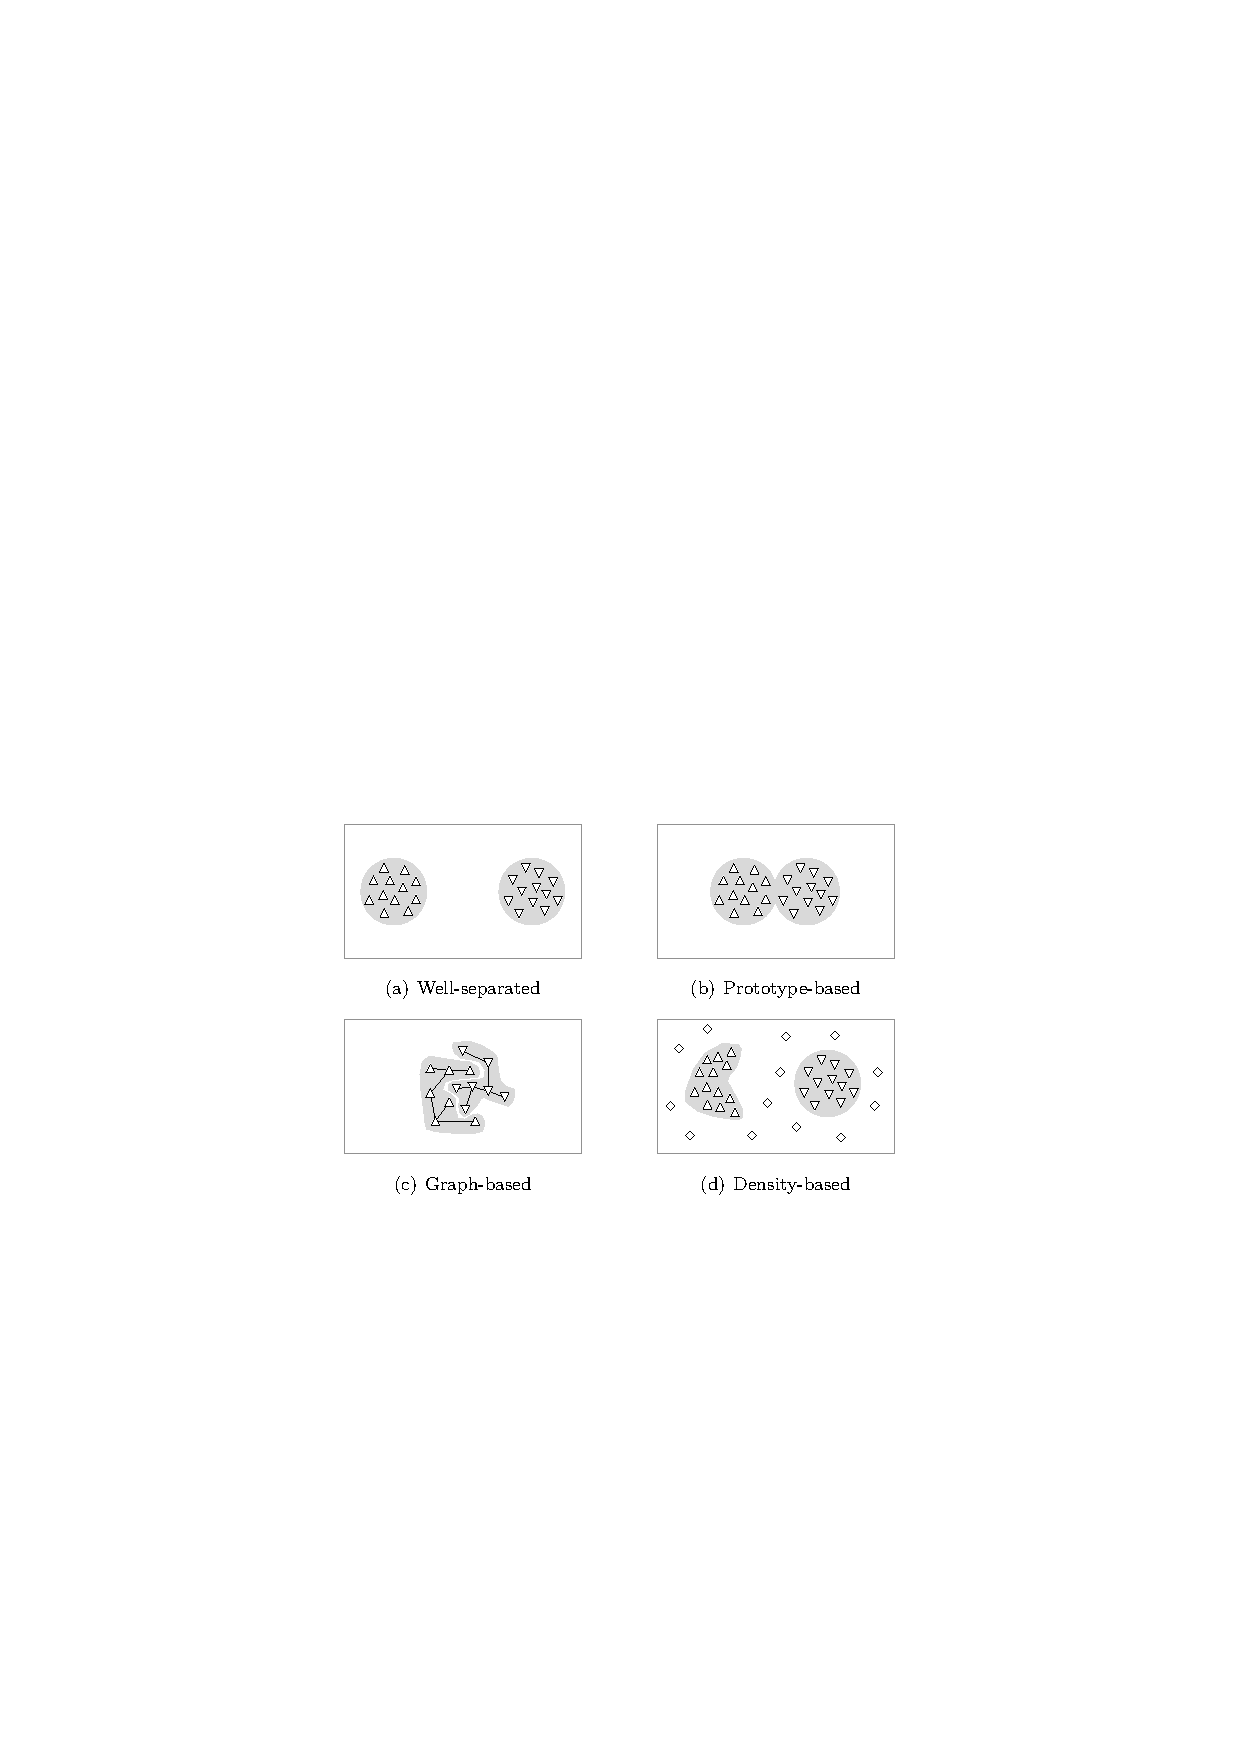
\includegraphics[width=0.75\textwidth]{figures/cluster_types.pdf}
    \caption{Types of clusters: (a) Well-separated, (b) Prototype-based, (c) Graph-based, (d) Density-based~\cite[p 9]{Meert06clustermaps}.}
    \label{fig:clusters}
  \end{center}
\end{figure}



\subsection{Clustering techniques}
\label{chapter:clustering-techniques}

Literature research reveals classifications of clustering techniques according to various aspects. Jain, Murty and Flynn primarily group the algorithms into hierarchical and partitional ones~\cite{Jain99clusterreview}. On the other hand, Stein and Busch split them into hierarchical, iterative, density-based and meta-search-controlled~\cite{Stein05density}. The differentiation of properties into groupings of clustering techniques and cross-cutting aspects is inconsistent among publications. This again shows the wide variety in which cluster analysis is being discussed and developed.

\begin{figure}[h]
  \begin{center}
    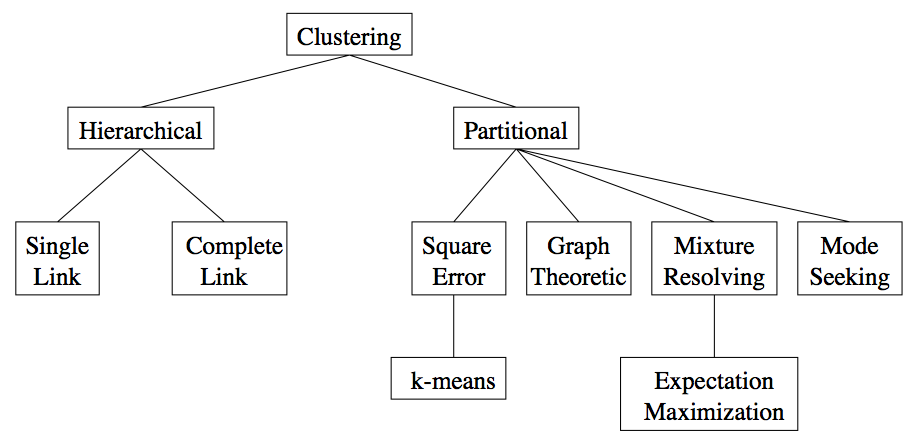
\includegraphics[width=0.9\textwidth]{figures/clustering_approaches_jain.png}
    \caption{A taxonomy of clustering approaches.~\cite[p 275]{Jain99clusterreview}.}
    \label{fig:clusters}
  \end{center}
\end{figure}

\begin{figure}[h]
  \begin{center}
    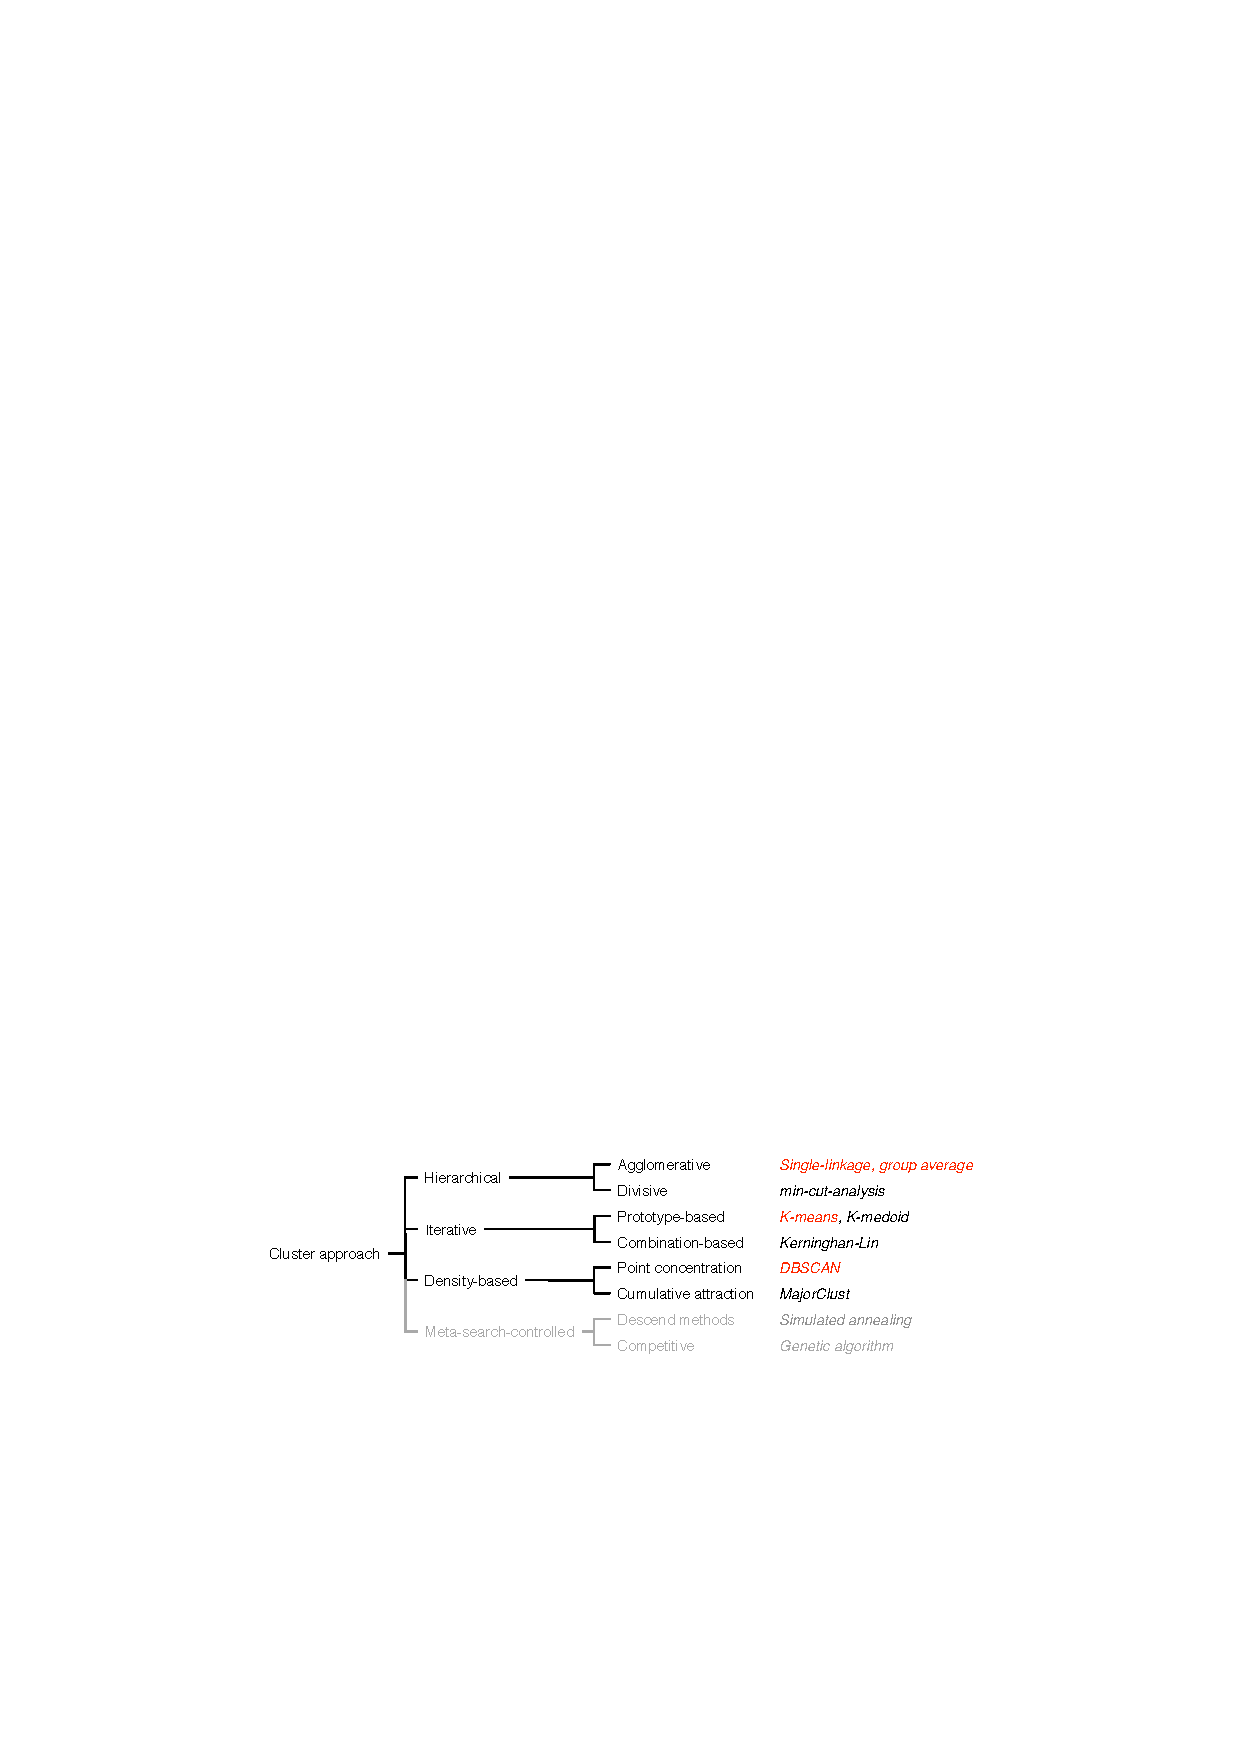
\includegraphics[width=1\textwidth]{figures/clustering_techniques_meert.pdf}
    \caption{A taxonomy of cluster algorithms as cited in~\cite[p 14]{Meert06clustermaps}, based on \cite{Stein05density}.}
    \label{fig:clusters}
  \end{center}
\end{figure}

\begin{itemize}

\item \textbf{Hierarchical versus Partitional}. Whether it is nested is the classic differentiation between clustering techniques. \textit{Partitional clustering} divides the data set into non-overlapping clusters. It usually is driven by an \textit{iterative} approach that optimized the result.
\textit{Hierarchical clustering} organizes clusters as a tree. Each node in the tree is the union of its children. Both clustering types are related: applying partitional clusterings in a sequence can lead to a hierarchical clustering and cutting the hierarchical tree at a particular level produces a partitional clustering~\cite{Meert06clustermaps}. 

An example of the relationship between hierarchical and partitional clustering is given by the following example of density-based algorithms. \textit{DBSCAN} produces simple data partitions and was further developed into \textit{OPTICS} which clusters data hierarchically~\cite{wiki:DBSCAN}.     

\item \textbf{Agglomerative versus divisive}. \textit{Agglomerative clustering} algorithms start with single items and successively merge them together into clusters. On the other hand, \textit{divisive clustering} algorithms begin with a single cluster that contains all items and splits it up until a stopping criterion is met. Each such merging or splitting procedure can be seen as one level in the hierarchical clustering tree~\cite{Jain99clusterreview}.

\item \textbf{Hard versus Fuzzy}. \textit{Hard clustering} algorithms assign every item to a single cluster, this means that the clustering is \textit{exclusive}. A \textit{fuzzy clustering} algorithm may attribute an item to multiple clusters in a \textit{non-exclusive way }by assigning degrees of membership. A fuzzy clustering may be converted into a hard clustering by assigning every data item to the cluster with the highest degree of membership~\cite{Jain99clusterreview, Meert06clustermaps}.

\item \textbf{Complete versus Partial}. With \textit{complete clustering}, assigning every point to a cluster is required. \textit{Partial clustering} relaxes this requirement so that not every point needs to be assigned to a cluster. This can be particularly useful when clustering data sets with outliers and noise. In such cases, the partial clustering can be used to focus on crowded areas~\cite{Jain99clusterreview}. 

\end{itemize}

Further aspects include monothetic versus polythetic and incremental versus non-incremental clustering techniques. 



\subsection{Proximity}
\label{chapter:proximity}

Similarity is fundamental to the definition of a cluster. In order to measure similarity, clustering algorithms evaluate their proximity. Continuous data requires different proximity measurements than categorical data.

For continuos data, the proximity between items is typically quantified by dissimilarity in terms of distance measures. The three main distance functions are visualized in figure~\ref{fig:clustering-proximity} and explained as follows\cite{Meert06clustermaps}:

\begin{figure}[h]
  \begin{center}
    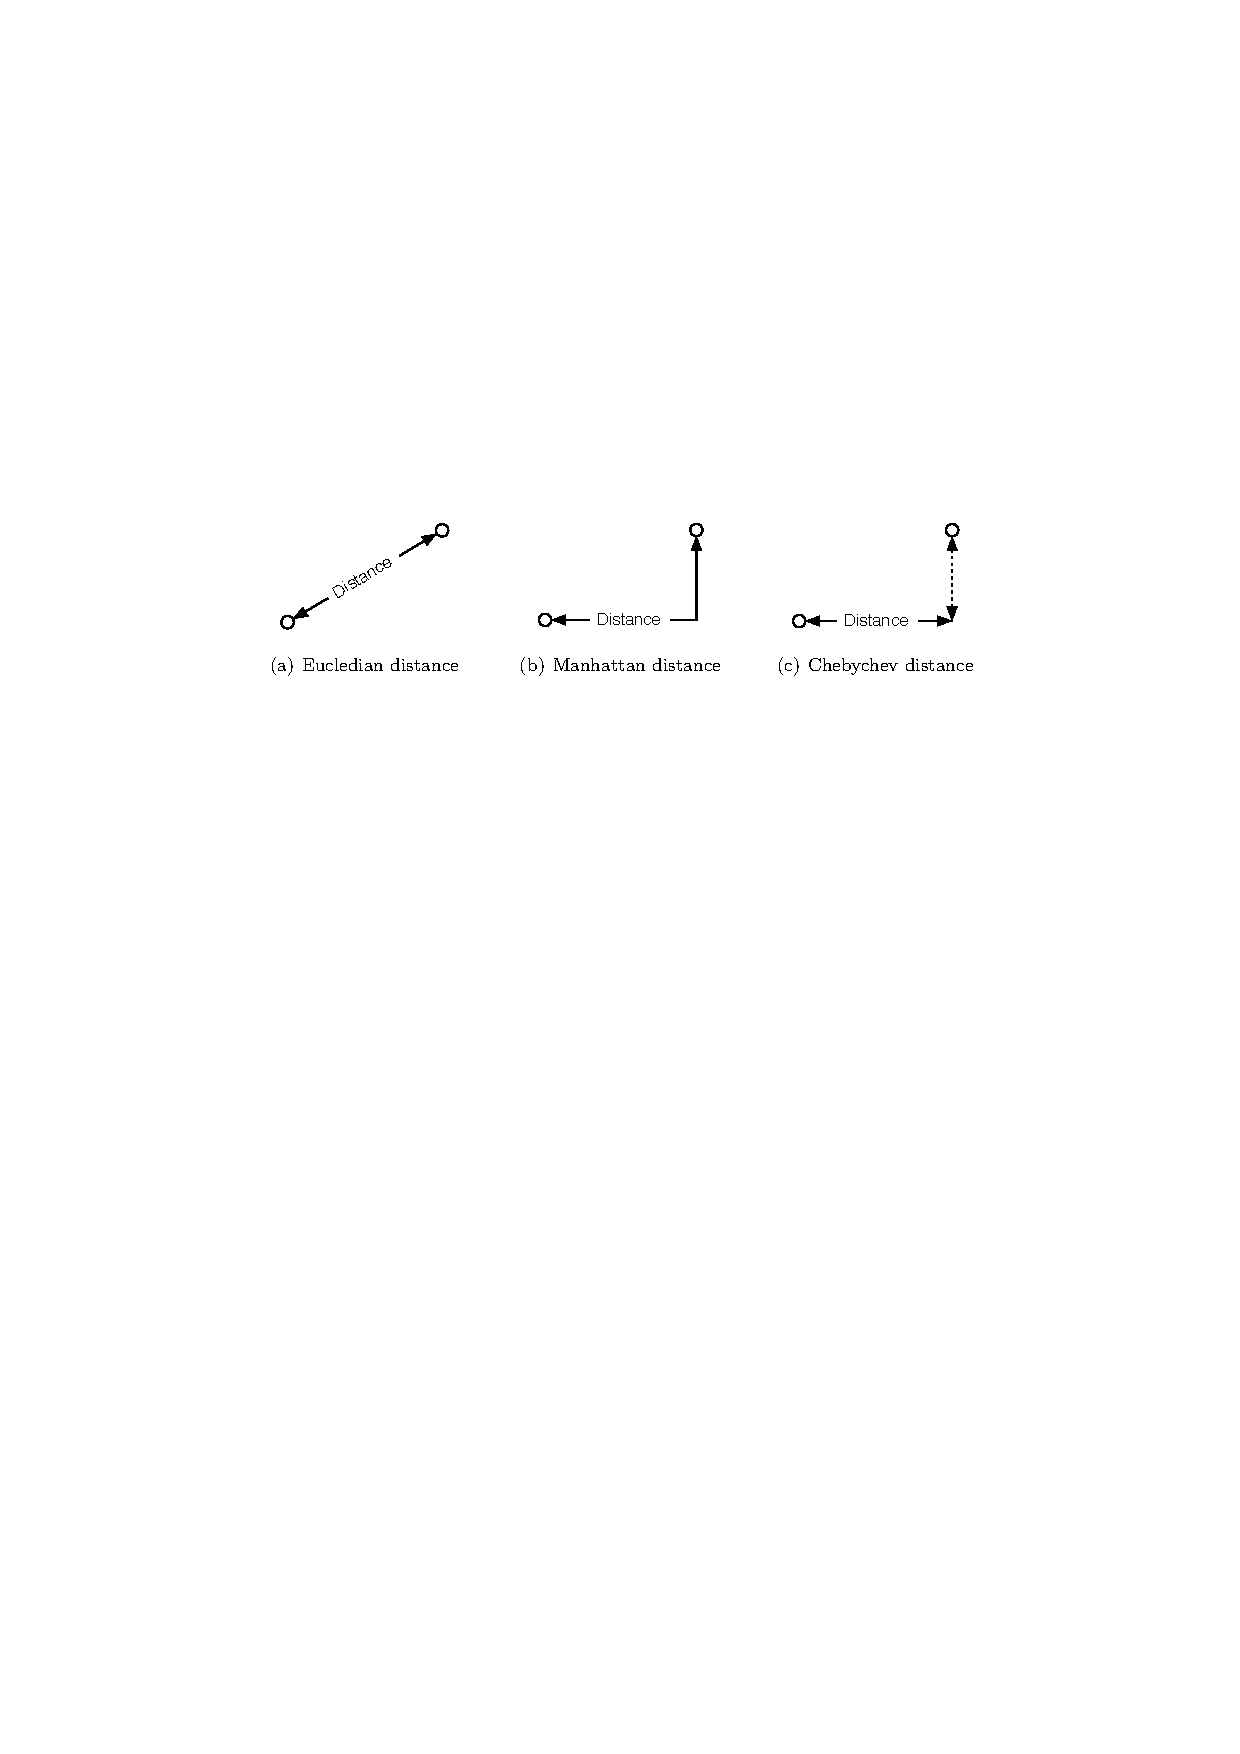
\includegraphics[width=1\textwidth]{figures/clustering_proximity.pdf}
    \caption{Distance measures for continuous data~\cite[p 12]{Meert06clustermaps}.}
    \label{fig:clustering-proximity}
  \end{center}
\end{figure}

\begin{itemize}

\item \textbf{Euclidian distance}. The euclidian distance is the geometric distance in the n-dimensional space. It is is the most common type of distance and defined as
\[ distance(x, y) = \sqrt{\sum_{i} (x_i - y_i)^2} \]

\item \textbf{Manhattan distance}. The manhattan distance, also known as city-block distance is distance when walking from one point to another following the axes. Compare with walking by following a raster like in manhattan. It is defined as
\[ distance(x, y) = \sum_{i} |x_i - y_i| \]

\item \textbf{Chebychev distance}. This distance measure returns the maximum distance between two points on any dimensions. It may be appropriate where two items are defined as `different', if they are different on any one of the dimensions.
\[ distance(x, y) = max |x_i - y_i| \]

\end{itemize}

\subsection{Clustering algorithms}

Researchers have created a multitude of algorithms, each appropriate for a certain task. As we will find out later, the requirements to the spatial clustering algorithm for this thesis are specific, which out-rules most scientific clustering algorithms which are geared towards image recognition or other disciplines. To provide an overview and to understand the basic differentiation of clustering techniques explained in \ref{chapter:clustering-techniques}, in this chapter we will introduce 3 foundational clustering algorithms: \textit{K-means}, \textit{Agglomerative Hierarchical Clustering Algorithm} and \textit{DBSCAN}.

\begin{itemize}

\item \textbf{Squared Error Algorithms: K-means}. The K-means is the most commonly used and simple algorithm based on a \textit{squared error criterion}. It creates a one-level partitioning of the data items by dividing them into \textit{K} clusters. By starting with a random initial partition it iteratively reassigns the patterns to clusters based on similarity.  The clustering process is completed when a convergence criterion is met, i.e. no further reassignments happen. Clusters are defined by \textit{cluster prototypes}: the centroid of the clustered items. Alternatively, the \textit{K-medoid} algorithm uses the most representative data item instead of the centroid.

The time complexity of the K-means algorithm is linear to the number of points:
\[time~complexity = \BigO{n}\]

\begin{algorithm}[t]
  \SetKwInOut{Input}{input}
  \Input{the number of clusters, $K$}
  \BlankLine
  {Select $K$ points as initial centroids}\;
  \While{Centroids do change}{
    {Form $K$ clusters by assigning each point to its closest centroid}\;
    {Recompute the centroid of each cluster}\;
  }
  \caption{K-means algorithm~\cite{Meert06clustermaps}}
  \label{alg:k-means}
\end{algorithm}

The selection of initial centroids affects the final outcome of the clustering process. Choosing them randomly is a simple but not very affective approach which can be compensating by applying multiple runs of the algorithm to retrieve an optimal result set. Optimizations to the centroid initialization include applying a hierarchical clustering or choosing distant points in the beginning.

Assigning points to the closest centroid requires a proximity measure, as explained in \ref{chapter:proximity}. Simple measures like the Euclidian distance are preferred, as this step needs to happen repeatedly within the algorithm. For each cluster, the centroid needs to be recalculated afterwards. This procedure is repeated until centroids do not change any more \cite{Jain99clusterreview, Meert06clustermaps}.

Figure \ref{fig:clustering_k-means} illustrates a K-means clustering process.

\begin{figure}[h]
  \begin{center}
    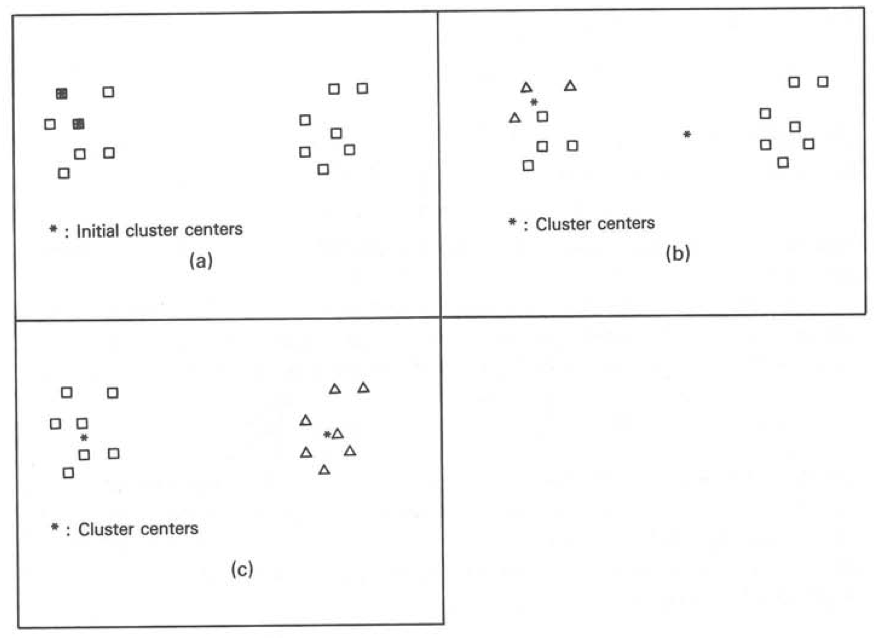
\includegraphics[width=0.9\textwidth]{figures/clustering_k-means.png}
    \caption{Convergence of K-means clustering: (a) initial data; (b) cluster membership after first loop; (c) cluster membership after second loop~\cite[p 99]{Jain88clustering}.}
    \label{fig:clustering_k-means}
  \end{center}
\end{figure}


\item \textbf{Agglomerative Hierarchical Clustering Algorithm}. This exemplary hierarchical clustering algorithm creates a hierarchy of nested sub clusters by serial partitioning. Its \textit{agglomerative} nature makes it start with every data item as a single clusters which get merged sub-sequentially. Alternatively, a \textit{divisive} hierarchical clustering would start with one cluster containing all data points and recursively split them up. At each level, a partitioning can be extracted, for example to serve as initial set of centroids for the previously discussed K-means algorithm. 

The time complexity of the agglomerative hierarchical clustering algorithm is:
\[time~complexity = \BigO{n^3}\]

\begin{algorithm}[t]
  {Assign each point to its individual cluster}\;
  {Compute the proximity matrix}\;
  \While{Number of clusters is larger than one}{
    {Merge the closest two clusters}\;
    {Update the proximity matrix to reflect the proximity between the new cluster and the original clusters}\;
  }
  \caption{Agglomerative hierarchic algorithm~\cite{Meert06clustermaps}}
  \label{alg:hierarchical}
\end{algorithm}

At the beginning of the agglomerative hierarchical clustering algorithm, each point is assigned to its own cluster. A proximity matrix is calculated that stores the distance of each pair of data item based on the chosen proximity measure.

To merge the two closest clusters, different heuristics may be applied. Most importantly, \textit{single-link} hierarchical clustering algorithms measure the distance between two clusters by the \textit{minimum} distance between all pairs of items from the two clusters. In contrast, \textit{complete-link} algorithms use the \textit{maximum} distance to create compact clusters and prevent chaining effects. Other approaches are based on \textit{average linkage} or \textit{Ward's method}. After merging the clusters, the proximity matrix will be updated so it reflects the current state of the clustering process. This procedure is repeated until all clusters have been merged, each step in the loop yields a level in the hierarchical clustering~\cite{Jain88clustering, Jain99clusterreview, Meert06clustermaps}.

Figure~\ref{fig:clustering-hierarchical-dendrogram} illustrates a Agglomerative Hierarchical clustering process as a dendrogram.

\begin{figure}[h]
  \begin{center}
    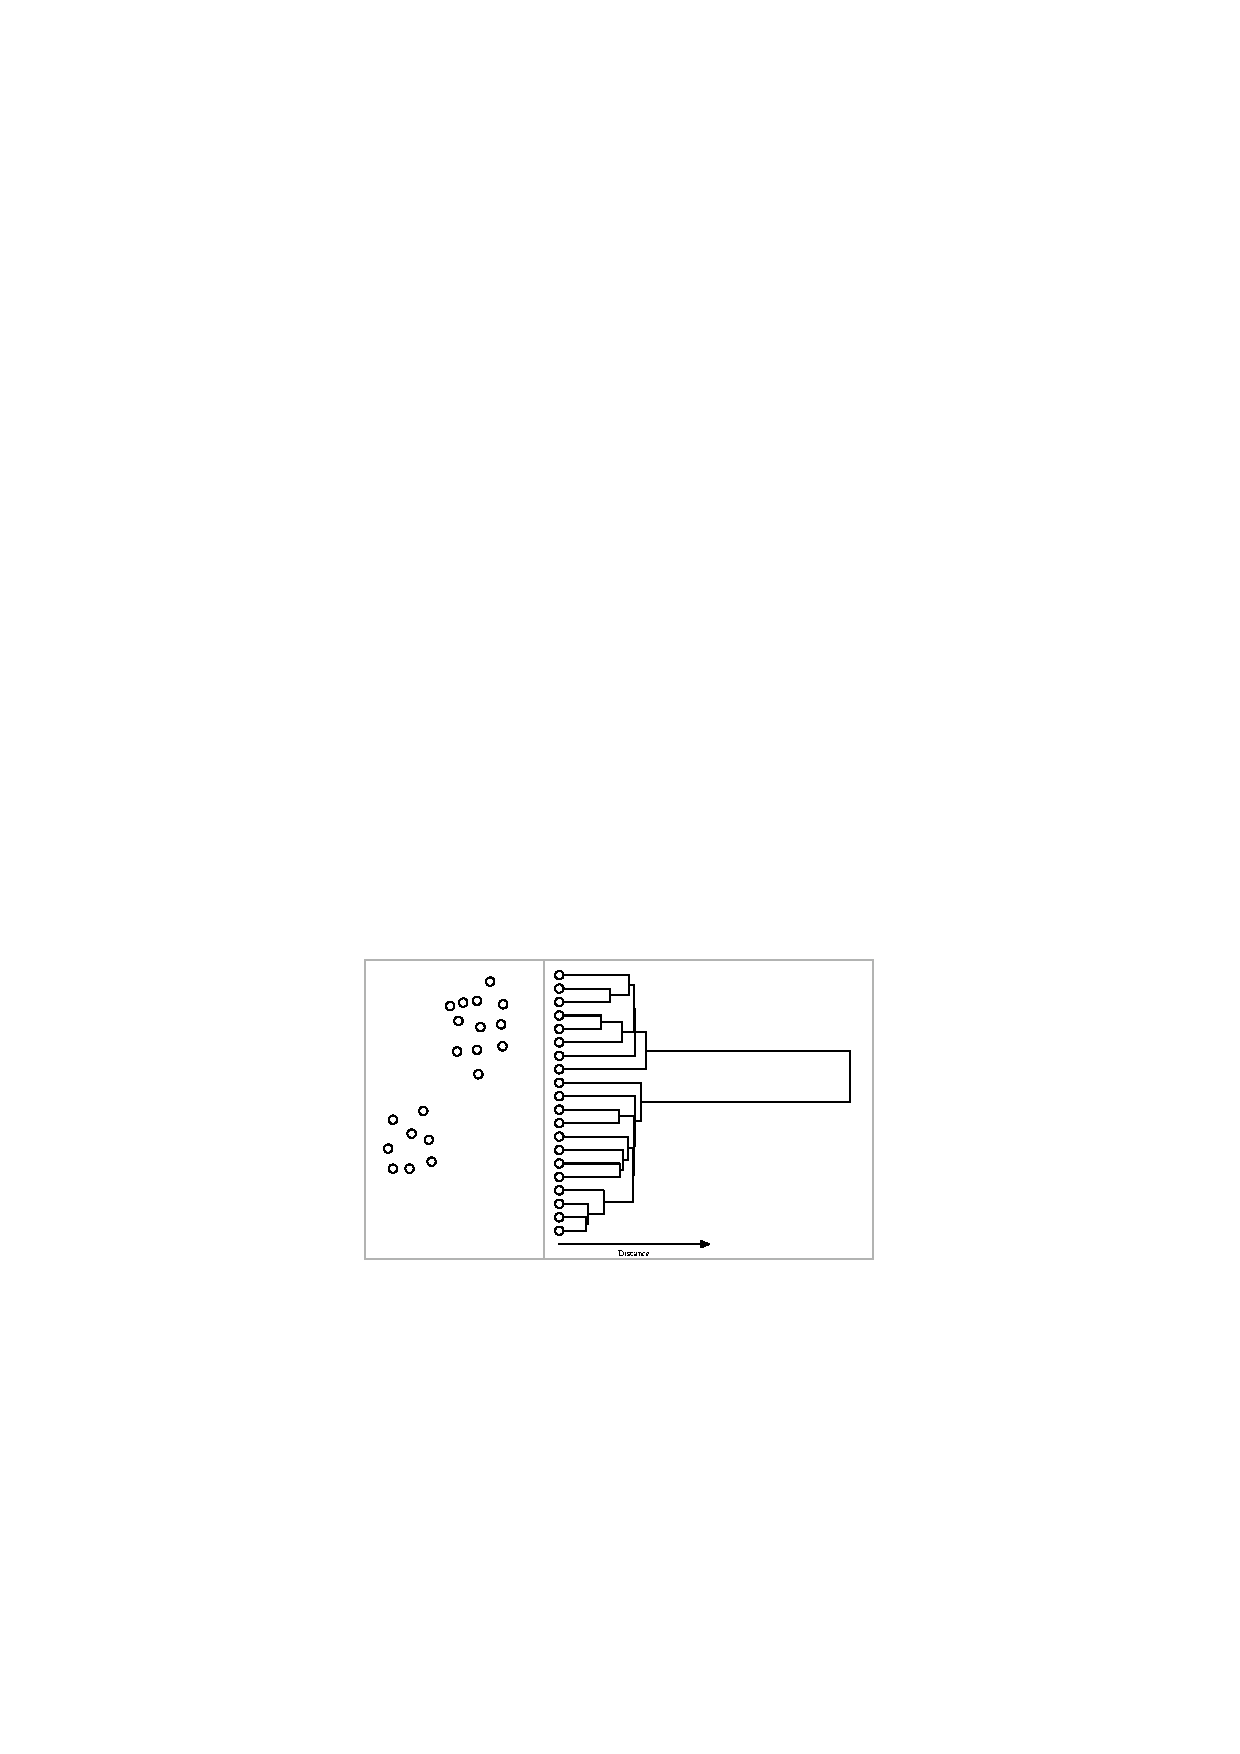
\includegraphics[width=0.9\textwidth]{figures/clustering_hierarchical_dendrogram.pdf}
    \caption{Dendrogram~\cite[p 20]{Meert06clustermaps}.}
    \label{fig:clustering-hierarchical-dendrogram}
  \end{center}
\end{figure}


\item \textbf{Density-based clustering algorithms: DBSCAN}. Density-based algorithms cluster regions of high density and separate them from regions with lower density. The density-based approach differentiates them from the previously discussed distance-based methods. This helps them overcome limitations of the former, as those tend to perform well in the detection of spherical-shaped clusters but perform weaker at discovering arbitrary shapes. Density-based algorithms are also insensitive to noise points, so that outliers get isolated. DBSCAN takes a center-based approach.
?
\begin{algorithm}[t]
  \While{Point is unclassified}{
    {Find points within region $\epsilon$}\;
    \If{number of points within region $> MinPts$} {
      {Start new cluster with Point}\;
      {Search regions of points in new cluster and expand cluster}\;
    }
  }
  \caption{DBSCAN algorithm~\cite{Meert06clustermaps}}
  \label{alg:dbscan}
\end{algorithm}

\textit{DBSCAN} starts with an unclassified point. Density is calculated by computing all points within a radius $\epsilon$. Based on the density, it classifies points as \textit{core points} if the number of points within neighborhood exceeds a threshold defined as $MinPts$. \textit{Border points} don't match the previous criterion but fall into the neighborhood of a core point. Finally \textit{noise points} are outside of any neighborhood and therefore are neither core points nor border points. Any core point will be expanded to a cluster in the procedure until every point has been classified~\cite{Varlaro08spatial, Meert06clustermaps}.

The quadratic time complexity of DBSCAN \BigO{n^2} can be optimized by using an indexing structure for the neighborhood queries~\cite{wiki:DBSCAN}:
\[time~complexity = \BigO{n \log{n} }\]



Figure~\ref{fig:clustering-dbscan} illustrates a DBSCAN clustering process.

\begin{figure}[h]
  \begin{center}
    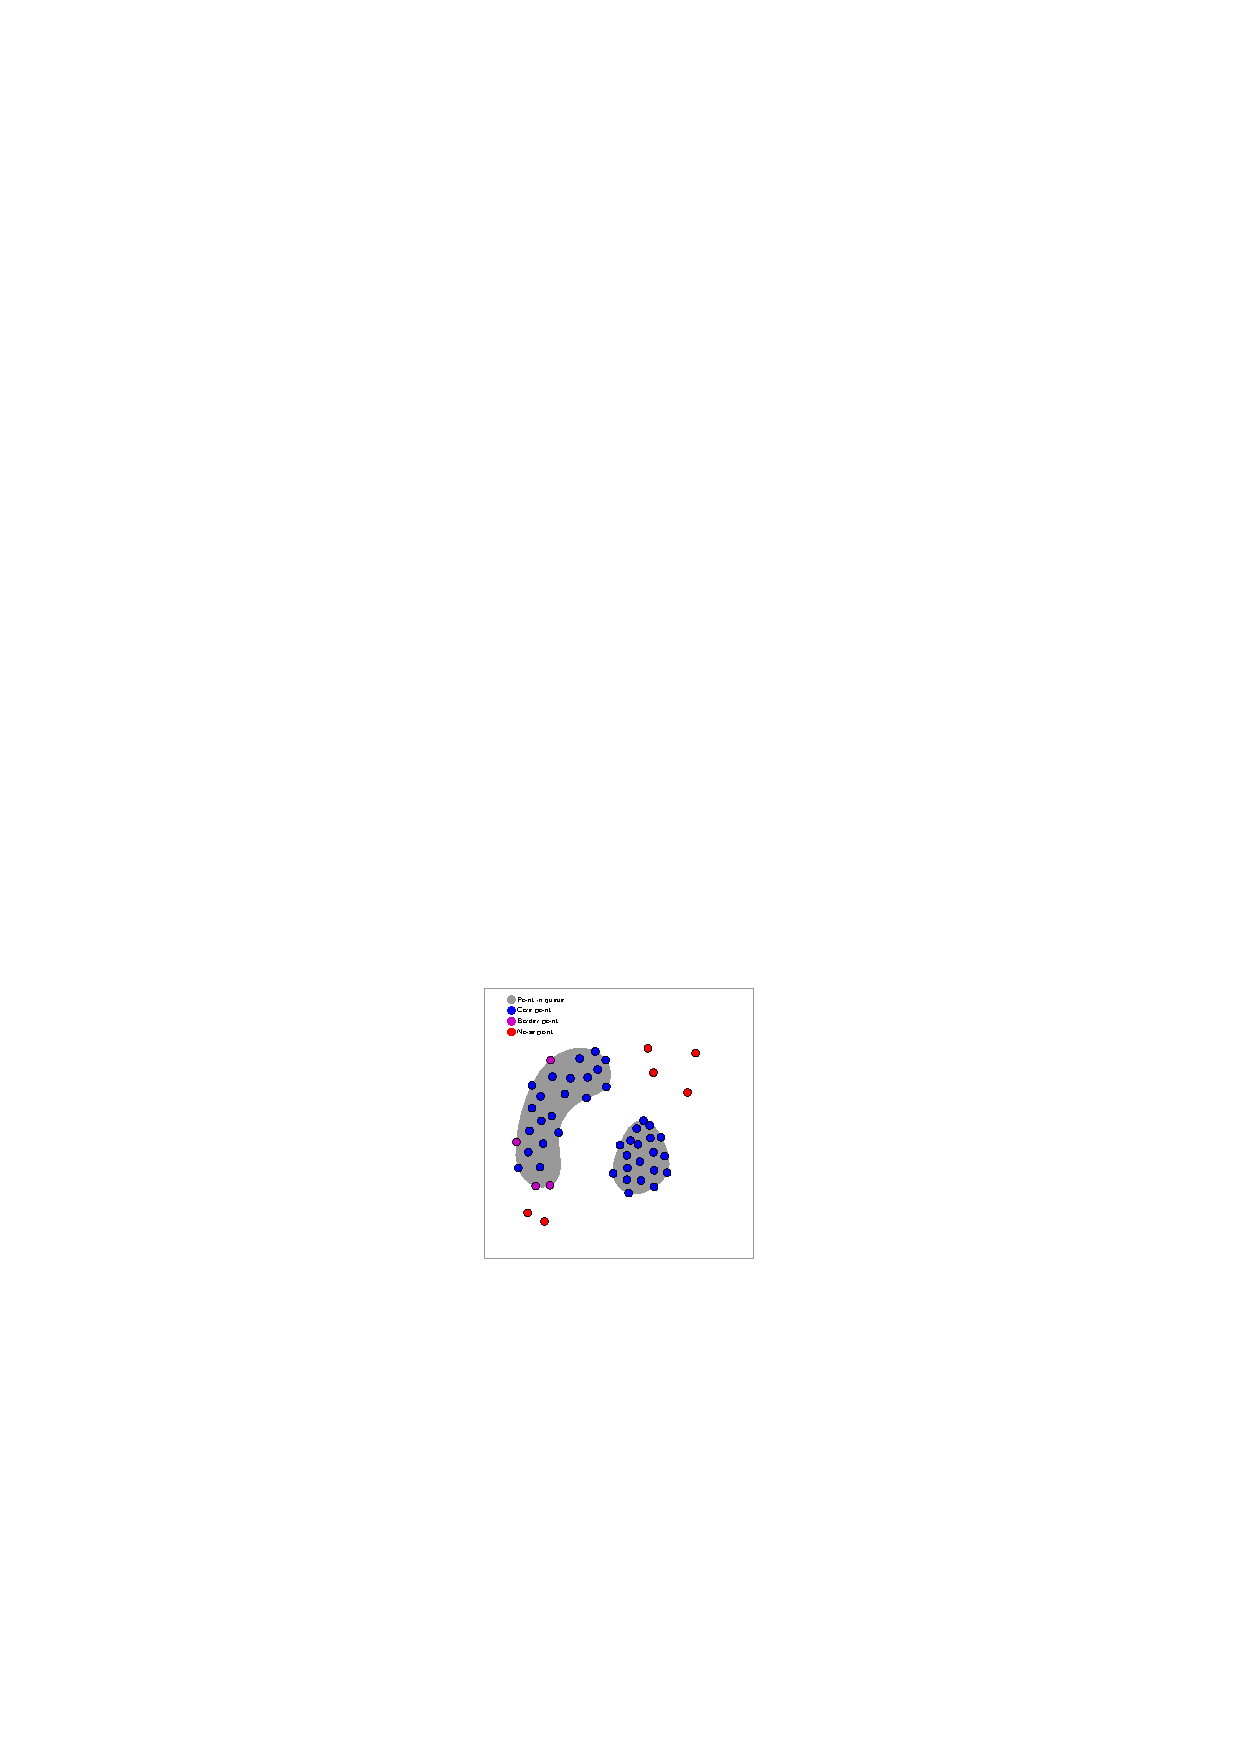
\includegraphics[width=0.55\textwidth]{figures/clustering_dbscan.pdf}
    \caption{DBSCAN algorithm~\cite[p 26]{Meert06clustermaps}.}
    \label{fig:clustering-dbscan}
  \end{center}
\end{figure}

\item \textbf{Grid-based algorithms: STING}. 

\end{itemize}





























%
% foundations - clustering algorithms
%

\section{Clustering algorithms}

Researchers have created a multitude of algorithms, each appropriate for a certain task. As we will find out later, the requirements to the spatial clustering algorithm for this thesis are specific, which out-rules most scientific clustering algorithms which are geared towards image recognition or other disciplines. To provide an overview and to understand the basic differentiation of clustering techniques explained in \ref{chapter:clustering-techniques}, in this chapter we will introduce 4 foundational clustering algorithms:

\begin{itemize}
\item {K-means (Squared Error Algorithm)}
\item {Agglomerative Hierarchical Clustering Algorithm}
\item {DBSCAN (Density-based)}
\item {STING (Grid-based)}
\end{itemize}

\subsection{Squared Error Algorithms: K-means}
\label{chapter:k-means}

The K-means is the most commonly used and simple algorithm based on a \textit{squared error criterion}. It creates a one-level partitioning of the data items by dividing them into \textit{K} clusters. By starting with a random initial partition, it iteratively reassigns the patterns to clusters based on similarity.  The clustering process is completed when a convergence criterion is met, i.e. no further reassignments happen. Clusters are defined by \textit{cluster prototypes}: the centroid of the clustered items. Alternatively, the \textit{K-medoid} algorithm uses the most representative data item instead of the centroid.

The time complexity of the K-means algorithm is linear to the number of points:
\[time~complexity = \BigO{n}\]

\begin{algorithm}[t]
  \SetKwInOut{Input}{input}
  \Input{the number of clusters, $K$}
  \BlankLine
  {Select $K$ points as initial centroids}\;
  \While{Centroids do change}{
    {Form $K$ clusters by assigning each point to its closest centroid}\;
    {Recompute the centroid of each cluster}\;
  }
  \caption{K-means algorithm~\cite{Meert06clustermaps}}
  \label{alg:k-means}
\end{algorithm}

The selection of initial centroids affects the final outcome of the clustering process. Choosing them randomly is a simple, but not very affective approach. This can be compensated by applying multiple runs of the algorithm, to retrieve an optimal result set. Optimizations to the centroid initialization include applying a hierarchical clustering or selecting distant points in the beginning.

Assigning points to the closest centroid requires a proximity measure, as explained in \ref{chapter:proximity}. Simple measures like the Euclidian distance are preferred, as this step needs to happen repeatedly within the algorithm. For each cluster, the centroid needs to be recalculated afterwards. This procedure is repeated until centroids do not change any more \cite{Jain99clusterreview, Meert06clustermaps}.

Figure \ref{fig:clustering_k-means} illustrates a K-means clustering process.

\begin{figure}[h]
  \begin{center}
    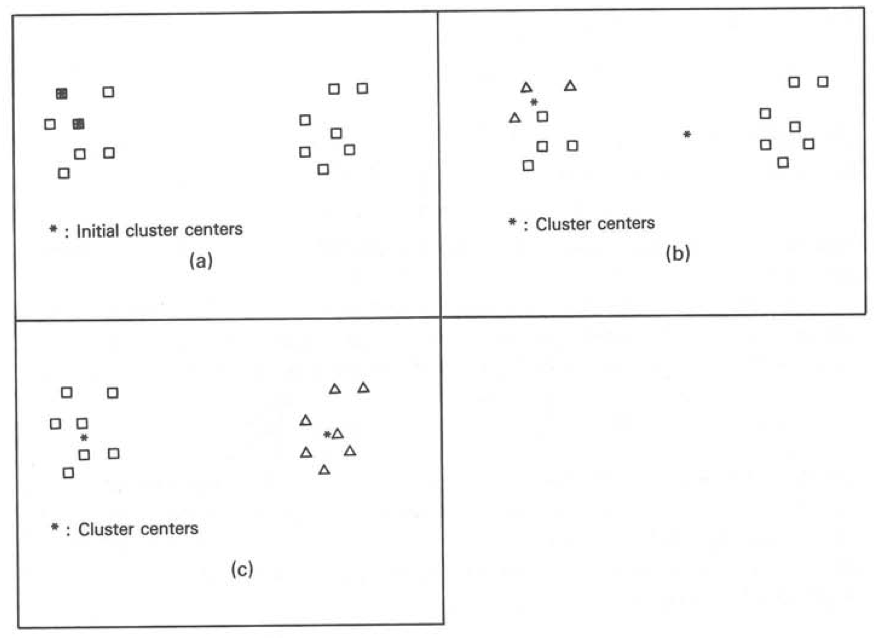
\includegraphics[width=1\textwidth]{figures/clustering_k-means.png}
    \caption{Convergence of K-means clustering: (a) initial data; (b) cluster membership after first loop; (c) cluster membership after second loop~\cite[p 99]{Jain88clustering}.}
    \label{fig:clustering_k-means}
  \end{center}
\end{figure}


\subsection{Agglomerative Hierarchical Clustering Algorithm}
\label{chapter:clustering-hierarchical}

This exemplary, \textit{hierarchical clustering algorithm} creates a hierarchy of nested sub clusters by serial partitioning. Its \textit{agglomerative} nature makes it start with every data item as a single cluster and merge them sub-sequentially. As an alternative, a \textit{divisive} hierarchical clustering would start with one cluster containing all data points and recursively split them up. At each level, a partitioning can be extracted, for example to serve as initial set of centroids for the previously discussed K-means algorithm. 

The time complexity of the agglomerative hierarchical clustering algorithm is:
\[time~complexity = \BigO{n^3}\]

\begin{algorithm}[t]
  {Assign each point to its individual cluster}\;
  {Compute the proximity matrix}\;
  \While{Number of clusters is larger than one}{
    {Merge the closest two clusters}\;
    {Update the proximity matrix to reflect the proximity between the new cluster and the original clusters}\;
  }
  \caption{Agglomerative hierarchic algorithm~\cite{Meert06clustermaps}}
  \label{alg:hierarchical}
\end{algorithm}

At the beginning of the agglomerative hierarchical clustering algorithm, each point is assigned to its own cluster. A proximity matrix is calculated to store the distances for all pairs of data items based on the chosen proximity measure.

To merge the two closest clusters, different heuristics may be applied. Most importantly, \textit{single-link} hierarchical clustering algorithms measure the distance between two clusters by the \textit{minimum} distance between all pairs of items from the two clusters. In contrast, \textit{complete-link} algorithms use the \textit{maximum} distance to create compact clusters and prevent chaining effects. Other approaches are based on \textit{average linkage} or \textit{Ward's method}. After merging the clusters, the proximity matrix will be updated, so that it reflects the current state of the clustering process. This procedure is repeated until all clusters have been merged, each step in the loop yields a level in the hierarchical clustering~\cite{Jain88clustering, Jain99clusterreview, Meert06clustermaps}.

Figure~\ref{fig:clustering-hierarchical-dendrogram} illustrates a Agglomerative Hierarchical clustering process as a dendrogram.

\begin{figure}[h]
  \begin{center}
    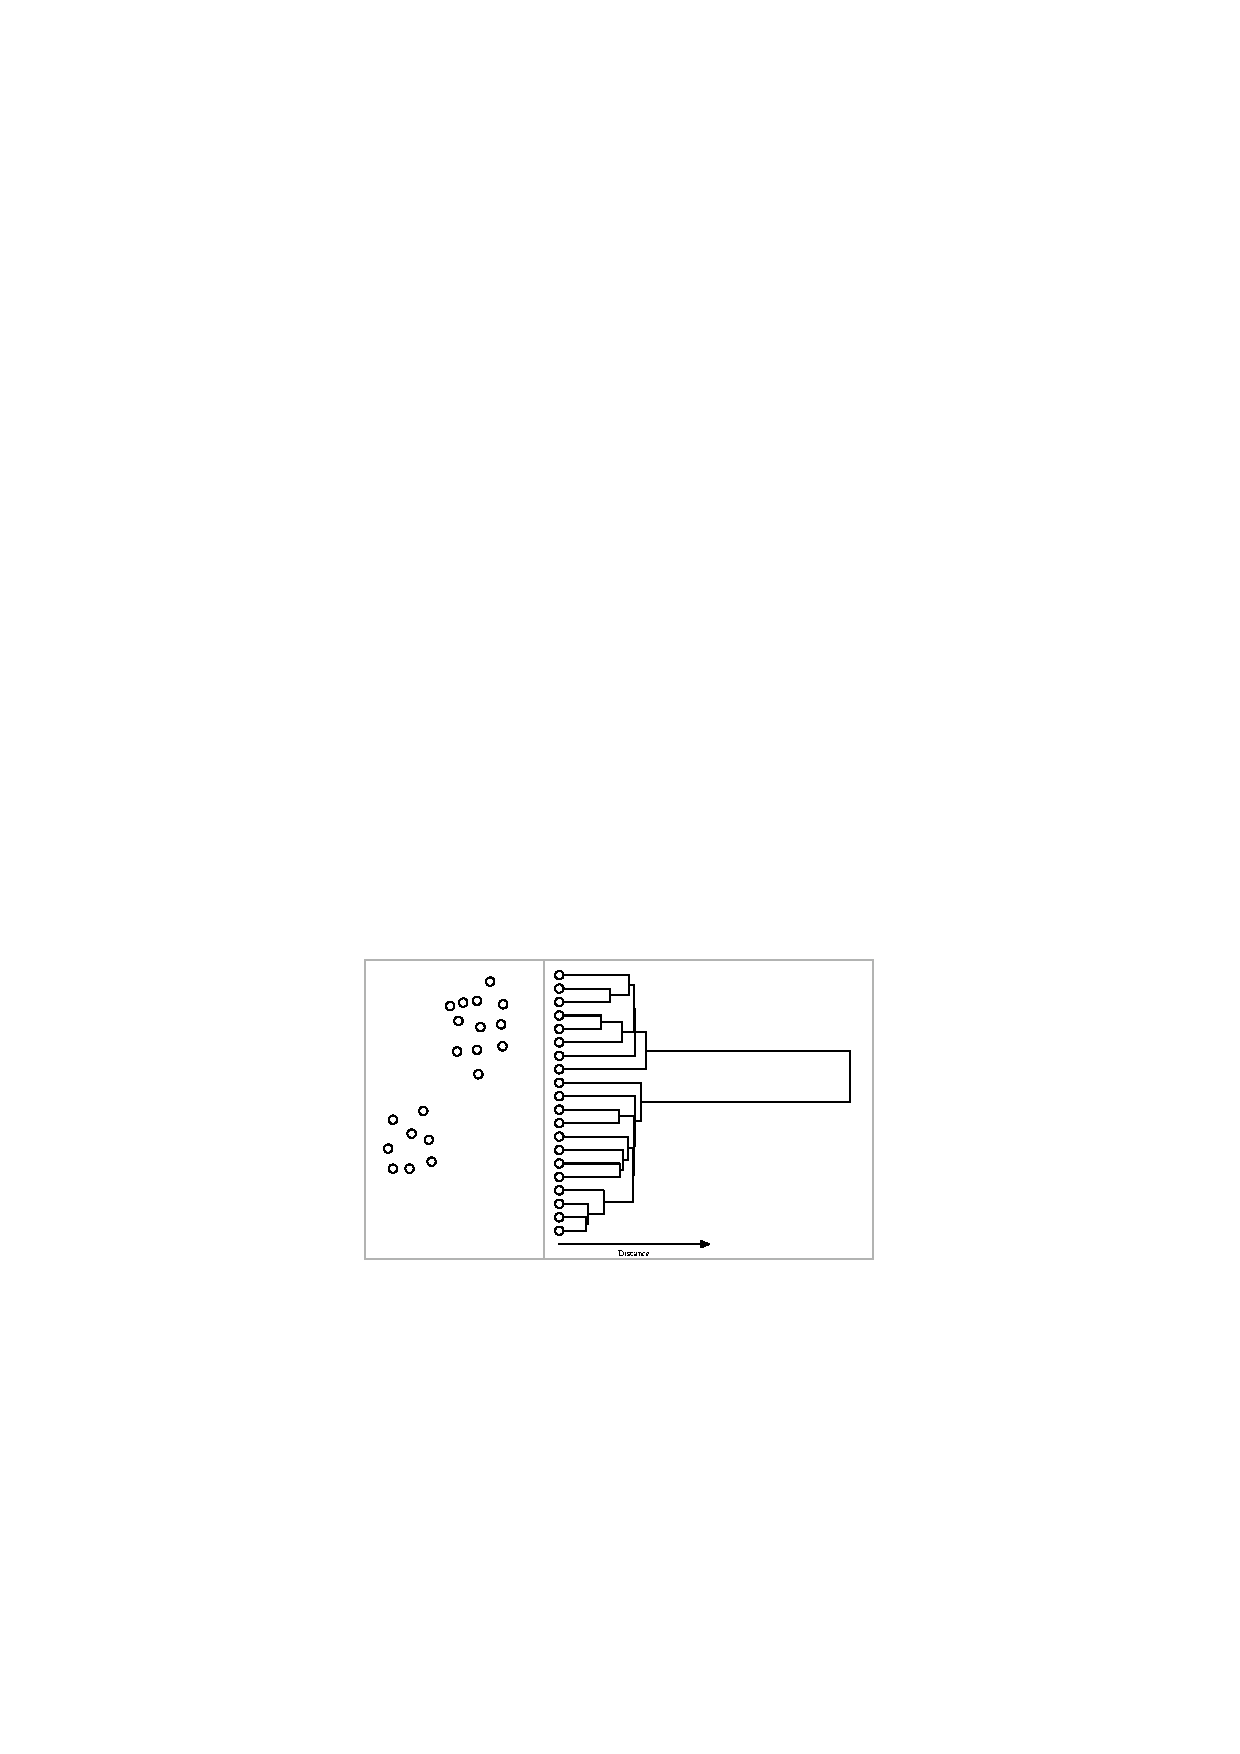
\includegraphics[width=0.9\textwidth]{figures/clustering_hierarchical_dendrogram.pdf}
    \caption{Dendrogram~\cite[p 20]{Meert06clustermaps}.}
    \label{fig:clustering-hierarchical-dendrogram}
  \end{center}
\end{figure}


\subsection{Density-based clustering algorithms: DBSCAN}

Density-based algorithms cluster regions of high density and separate them from regions with lower density. The density-based approach is different to the previously discussed distance-based methods. Those tend to perform well in the detection of spherical-shaped clusters, but discovering arbitrary shapes is a problem. Density-based algorithms overcome this limitation and are also insensitive to noise points, so that outliers get isolated.

\begin{algorithm}[t]
  \While{Point is unclassified}{
    {Find points within region $\epsilon$}\;
    \If{number of points within region $> MinPts$} {
      {Start new cluster with Point}\;
      {Search regions of points in new cluster and expand cluster}\;
    }
  }
  \caption{DBSCAN algorithm~\cite{Meert06clustermaps}}
  \label{alg:dbscan}
\end{algorithm}

\textit{DBSCAN} starts with an unclassified point. Subsequently, the density of the point is calculated by computing all its neighborhood points within a radius $\epsilon$. Based on the density, the algorithm classifies points as \textit{core points}, \textit{border points} or \textit{noise points}:

\begin{itemize}
\item \textit{core points} have a number of points within their neighborhood that exceeds the threshold defined as $MinPts$
\item \textit{border points} don't match the previous criterion but they themselves fall into the neighborhood of another core point
\item \textit{noise points} are outside of any neighborhood and therefore are neither core points nor border points
\end{itemize}

Any core point will be expanded to a cluster in the procedure until every point has been classified~\cite{Varlaro08spatial, Meert06clustermaps}.

The quadratic time complexity of DBSCAN \BigO{n^2} can be optimized by using an indexing structure for the neighborhood queries~\cite{wiki:DBSCAN}:
\[time~complexity = \BigO{n \log{n} }\]

Figure~\ref{fig:clustering-dbscan} illustrates a DBSCAN clustering process.

\begin{figure}[h]
  \begin{center}
    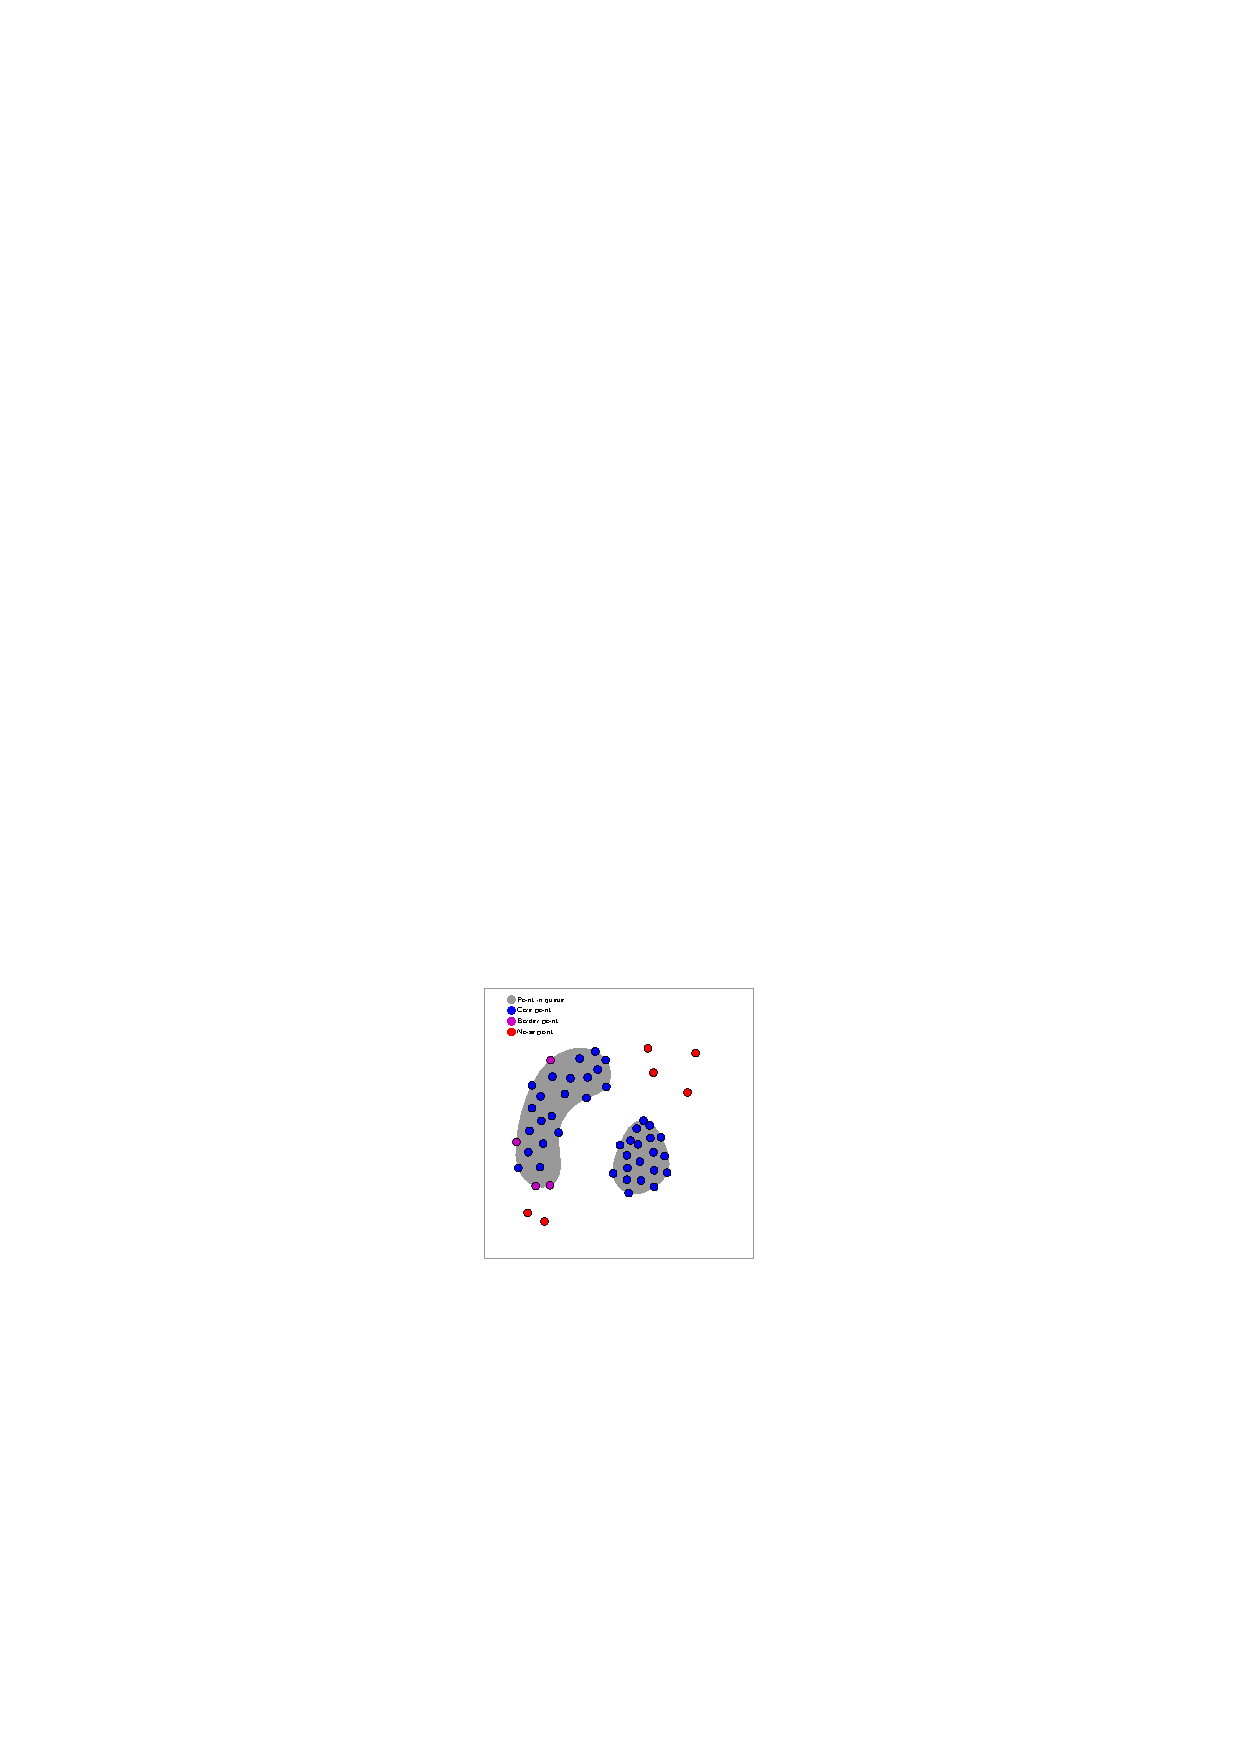
\includegraphics[width=0.55\textwidth]{figures/clustering_dbscan.pdf}
    \caption{DBSCAN algorithm~\cite[p 26]{Meert06clustermaps}.}
    \label{fig:clustering-dbscan}
  \end{center}
\end{figure}

\subsection{Grid-based algorithms: STING}
\label{chapter:clustering-grid}

The time complexity of the previously discussed algorithms is at least linear to the number of points that have to be clustered. Grid-based algorithms overcome this performance limitation by partitioning data to be clustered in a grid structure. The clustering process is executed on pre clustered cells of the grid structure, which obviously scales better.

The STING algorithm takes such a grid-based approach and divides the data points into a grid of rectangular cells. The cells form a hierarchical structure, so that different levels of grids correspond to different resolutions. Every cell in the grid is sub-divided into a further partitioning one level deeper in the hierarchy. STING therefore precomputes a hierarchical index with various levels of granularity on which the clustering process is later executed. The name-giving property of STING (Statistical INformation Grid) is that each cell contains statistical information which can be used to answer queries. 

The time complexity can be shifted to the computation of the grid which is linear to the points of data $\BigO{n}$. The query processing time is reduced to $\BigO{g}$, where $g$ is the constant of number of cells at the bottom level of the computed hierarchy. As per the construction of the hierarchy, it can be assumed that $g \ll n$~\cite{Varlaro08spatial, Wang97sting}.  

Figure~\ref{fig:clustering-sting} illustrates a hierarchical grid used in the STING clustering process.

\begin{figure}[h]
  \begin{center}
    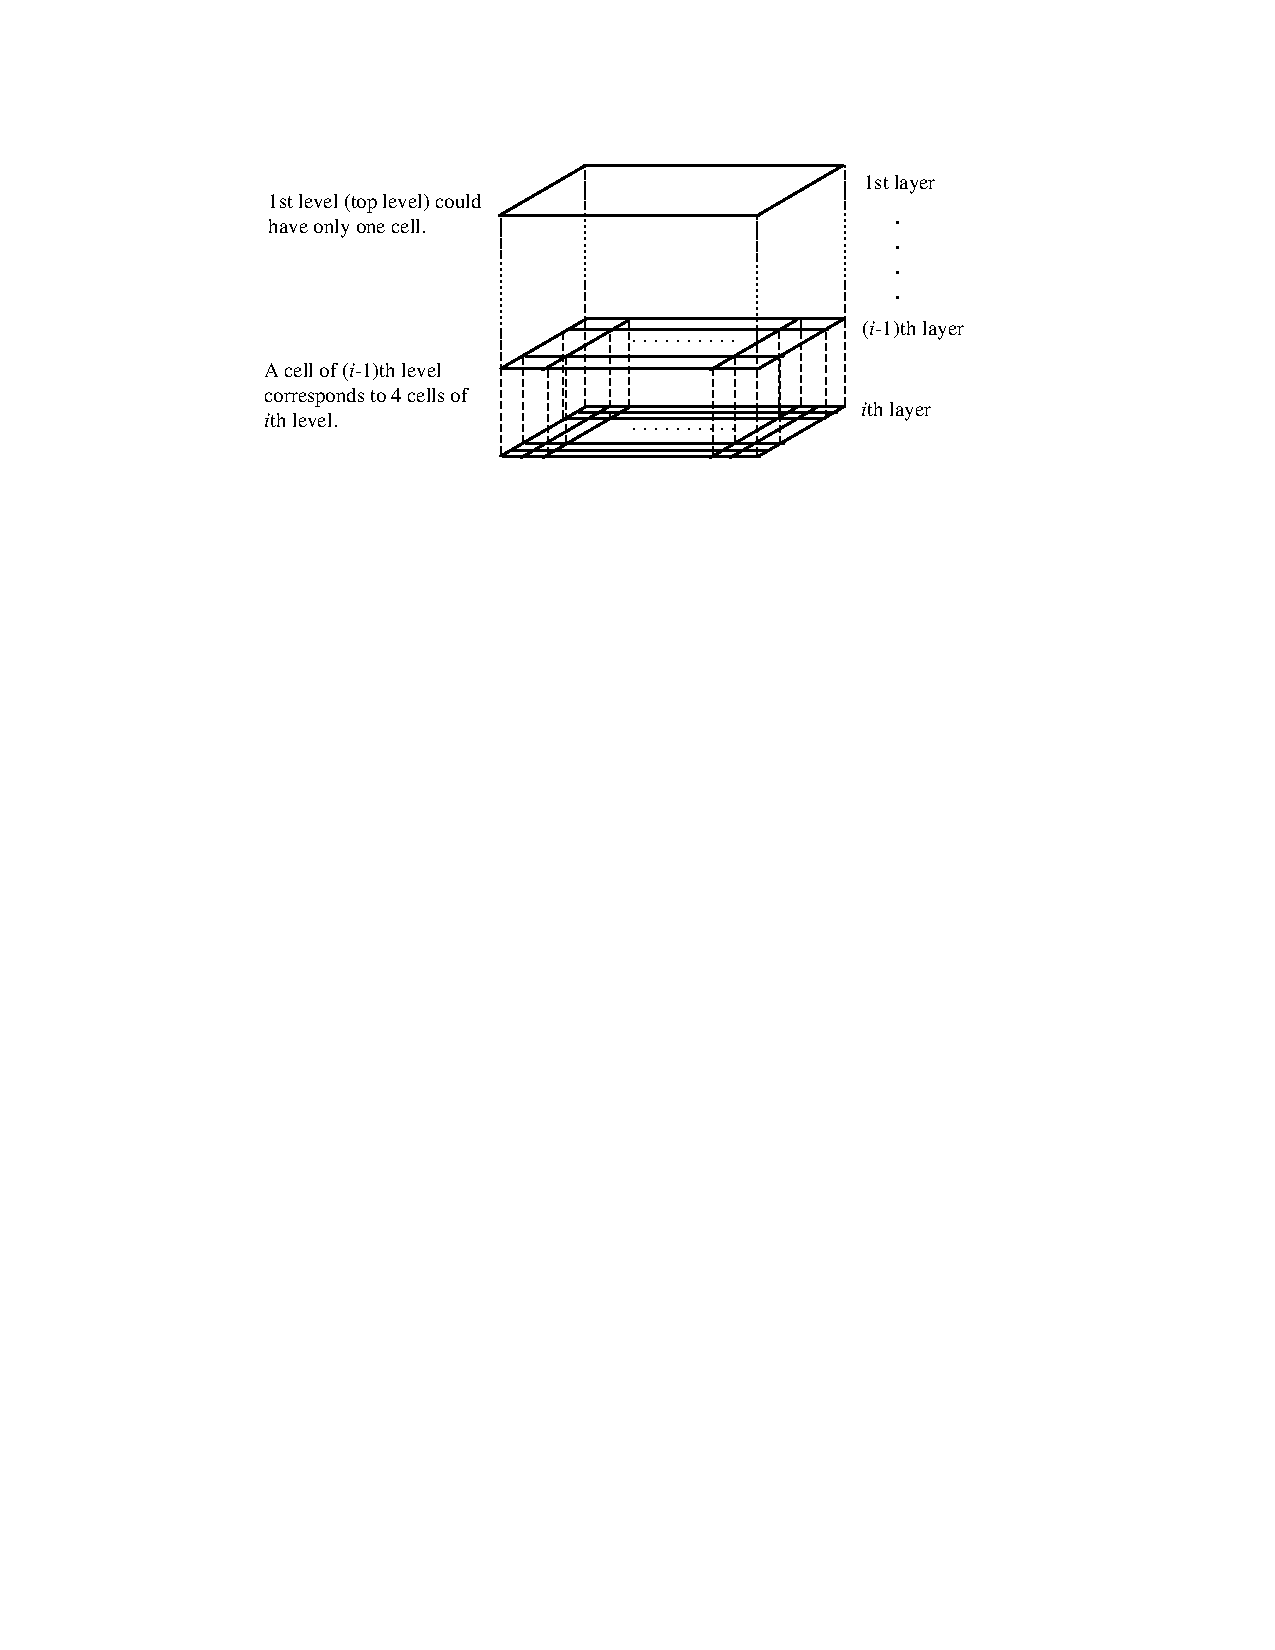
\includegraphics[width=0.9\textwidth]{figures/clustering_sting.pdf}
    \caption{Hierarchical Structure of the STING algorithm~\cite[p 5]{Wang97sting}.}
    \label{fig:clustering-sting}
  \end{center}
\end{figure}























%
% foundations - spatial data
%

\section{Spatial data}
\label{chapter:spatial-data}

A central aspect in web mapping is dealing with spatial data. Decisions on how to structure and store spatial data highly influence the computation tasks that may be performed on such data. This mainly depends on the type of spatial data, where points are the most basic of all. Depending on the use case, different types of data are to be represented and stored: points, lines, rectangles, regions, surfaces and/or volumes. While most of the discussed concepts may be extended or generalized for processing more complex types of data, this is out of scope for this thesis. Instead, we focus on points as the most common type of spatial data~\cite{Samet90spatialdata}.

One fundamental way to store spatial data is the quadtree, a hierarchical data structure based on recursive decomposition of space. Hanan Samet attributes the history of quadtrees (and octrees which are their 3-dimensional extension) to Dijkstra, who invented a one-level decomposition of a matrix into square blocks. Morton then applied this technique to creating a spatial index (z-order). We will first discuss space orders \& decomposition and then put those into context when outlining the basics of the quadtree.


\subsection{Space order methods}
\label{chapter:space-order}

In order to store multi-dimensional, spatial data in a sequential storage like computer memory, the data needs to be serialized. Consider a pixel image as an example. Its 2-dimensional pixel values are positioned in planar space. In order to store the image, those pixels have to be processed in a predefined order, such that they can be serialized into a 1-dimensional array of memory units.

The traditional order for storing a raster of image data was row by row. The row order sequentially processes the raster row by row from left to right, starting at the top left corner. In contrast, the row-prime order switches the horizontal processing direction at the end of each row. This leads to a higher locality as it has the property of always moving to a 4-neighbor~\cite{Goodchild83raster}.

Besides the discussed row orders, additional space-ordering methods have been developed to serve different purposes. The Morton and Peano-Hilbert orders both visit entire sub quadrants first before before exiting them. The Morton order is easier to compute, because the position (key) of each element in the ordering can be determined by interleaving the bits of the x and y coordinates of that element. One disadvantage of the Morton order are the gaps: the longest move in a raster of $2^n$ by $2^n$ is one column and $2^n - 1$ rows (or vice versa). A better locality is offered by the Hilbert-Peano order which always has the property of moving to a 4-neighbor. This advantage on the other hand has the cost of a more complex definition. Calculating keys for the Hilbert-Peano order is more difficult. The higher complexity of the Hilbert-Peano obviously shows that its recursion is harder to define as well. Figure~\ref{fig:space-orders} illustrates these fundamental space orders with two further ones that allow for ordering unbounded space in two (Cantor-diagonal order) or four directions (spiral order)~\cite{Samet90spatialdata}.

\begin{figure}[h]
  \begin{center}
    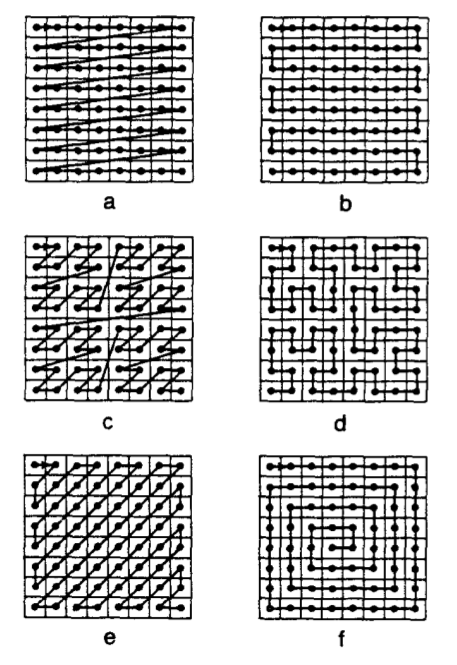
\includegraphics[width=0.5\textwidth]{figures/space_orders.png}
    \caption{The result of applying a number of different space-ordering methods to an $8 \times 8$ image whose first element is in the upper left corner of the image: (a) row order, (b) row-prime order, (c) Morton order, (d) Peano-Hilbert order, (e) Cantor-diagonal order, (f) spiral order~\cite[p 14]{Samet90spatialdata}.}
    \label{fig:space-orders}
  \end{center}
\end{figure}

The fact that the Hilbert-Peano order has the property of always moving to a 4-neighbor shouldn't be misinterpreted as still there are gaps. ``A bijective mapping from multidensional data to one dimension cannot be done the way that in any case nearby multidimensional points are also close together in one dimension~\cite{Tropf81multidimensional}''. Figure~\ref{fig:space-orders} clearly shows what Samet describes as ``both the Morton and Peano-Hilbert order exhaust a quadrant or subquadrant of a square image before exiting it~\cite{Samet90spatialdata}''. This means that the orders maintain locality for those quadrants based on the hierarchy, but the edges are still disconnected. The same issue will be dealt with further in Geohash (TODO Geohash).


\subsection{Space decomposition methods}

By definition, space decomposition methods partition space in a way so that,
\begin{itemize}
\item partitions are infinitely repetitive patterns for images of any size,
\item partitions are infinitely decomposable to generate finer sub-partitions of higher resolution.~\cite{Samet90spatialdata}
\end{itemize}

Various space decomposition methods exist. They can be classified depending on the shapes that are used for the partitioning patterns. Polygonal shapes are computationally simpler and can be used to approximate the interior of a region while non-polygonal shapes are more geared towards approximating the perimeter of region. Figure~\ref{fig:space-decomposition} visualizes a number of basic, polygon-based space decomposition methods. 

\begin{figure}[h]
  \begin{center}
    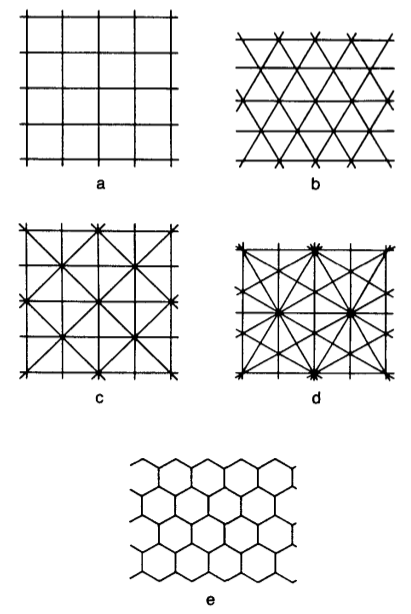
\includegraphics[width=0.5\textwidth]{figures/space_decompositions.png}
    \caption{Sample tessellations: (a) $[4^4]$ square; (b) $[6^3]$ equilateral triangle; (c) $[4.8^2]$ isoceles triangle; (d) $[4.6.12]$ 30-60 right triangle; (e) $[3^6]$ hexagon~\cite[p 17]{Samet90spatialdata}.}
    \label{fig:space-decompositions}
  \end{center}
\end{figure}

The simplest polygonal space decomposition method is based on squares. It is directly related to the Morton and Peano-Hilbert space order methods as described in the previous chapter \ref{chapter:space-order}. Both orders work in a hierarchical manner and visit entire sub-quadrants first before continuing further. This is why they are predestined to decomposing space into squares as indicated in Figures~\ref{fig:space-orders}~and~\ref{fig:space-decompositions}.

\subsection{Quadtree}

Quadtrees are hierarchical data structures based on recursive decomposition of space. Their original motivation was to optimize storage by aggregating identical or similar values. Over time they have also been studied to optimize execution time of spatial application and have been established as a common practice for representing and storing spatial data. The resolution of a quadtree can be fixed or variable and directly relates to the number of decomposition times of the space where the data points live. A standardized implementation is the region quadtree which subdivides space into four equal-sized quadrants.

\begin{figure}[h]
  \begin{center}
    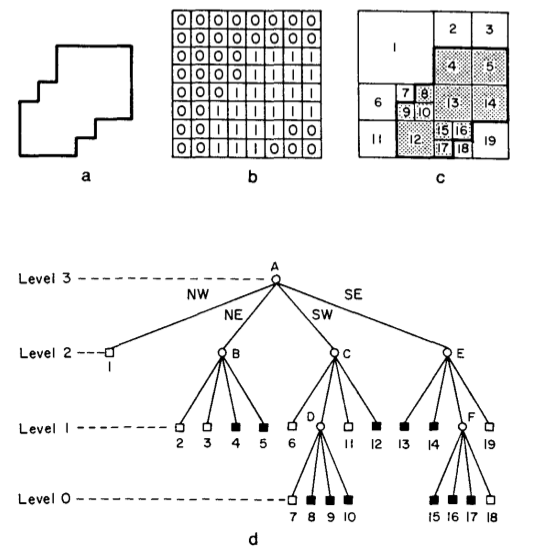
\includegraphics[width=0.7\textwidth]{figures/quadtree.png}
    \caption{An example of (a) a region, (b) its binary array, (c) its maximal blocks (blocks in the region are shaded), and (d) the corresponding quadtree~\cite[p 3]{Samet90spatialdata}.}
    \label{fig:space-decompositions}
  \end{center}
\end{figure}

Quadtrees can be constructed in different ways. A top-down approach implements the Morton order which maps the multidimensional data to one dimension and has been introduced in chapter~\ref{chapter:space-order}. Also note that the term quadtree has taken various meanings: actually it is a trie (or digital tree) structure because each data key is a sequence of characters. ``A node at depth $i$ in the trie represents an $M$-way branch depending on the $i$-th character'' \cite{Samet90spatialdata}.

\subsection{Geohash}
\label{chapter:geohash}

Geohash is a latitude/longitude geocode system based on the Morton order, described in \ref{chapter:space-order}. It encodes geographic point coordinates into string identifiers that reflect a hierarchical spatial structure. Its gradual precision degradation property means that if two geohashes share a common prefix, their closeness is described by the length of the shared prefix~\cite{wiki:geohash, Smiley11geohash}.

Originally, the geohash encoding algorithm has been developed and put into the public domain by Gustavo Niemeyer when creating the web service \href{http://geohash.org}{geohash.org}. The service allows to encode spatial coordinates into unique string identifiers and vice versa~\cite{wiki:geohash}. Amongst other applications, it has also been incorporated into geospatial search plugins of the Apache Solr search platform~\cite{Smiley11geohash} and leveraged for real-time, location-aware collaborative filtering of web content by HP Labs~\cite{Sand11geohashapp}.

A geohash is constructed by interleaving the bits of the latitude and longitude values and converting them into a string of characters using a Base 32 encoding. As every Base 32 symbol is represented by an uneven number of 5 bits, the resulting  space decomposition is a rectangular grid formed by $4 \times 8$ or $8 \times 4$ cells. The orientation of the resulting rectangles alternates between vertical for characters of an odd index and horizontal for such characters that are positioned at an even index within the geohash. Figure \ref{fig:geohash} illustrates how the first character of a geohash string splits the projected earth into an $8 \times 4$ grid of horizontally aligned rectangles~\cite{wiki:geohash, Smiley11geohash}.

\begin{figure}[h]
  \begin{center}
    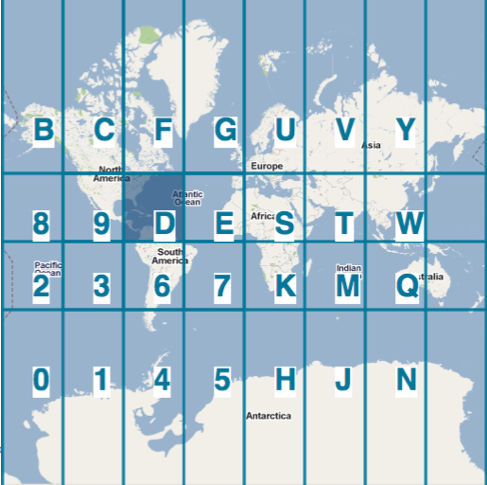
\includegraphics[width=0.7\textwidth]{figures/geohash_example.png}
    \caption{Space decomposition of the geohash algorithm on the first level~\cite{Smiley11geohash}.}
    \label{fig:geohash}
  \end{center}
\end{figure}

The fact that points with a common prefix are near each other must not be confused with the converse. Due to the nature of the morton order, edge cases exist. Two points may be very close to each other, without sharing an equally long prefix. Figure \ref{fig:geohash-edge} illustrates an example of two closely positioned points being located within different geohashes. The first point being at the very lower end of the ``DRT'' geohash and the second point positioned closely at the upper end of the ``DRM'' geohash. 

\begin{figure}[h]
  \begin{center}
    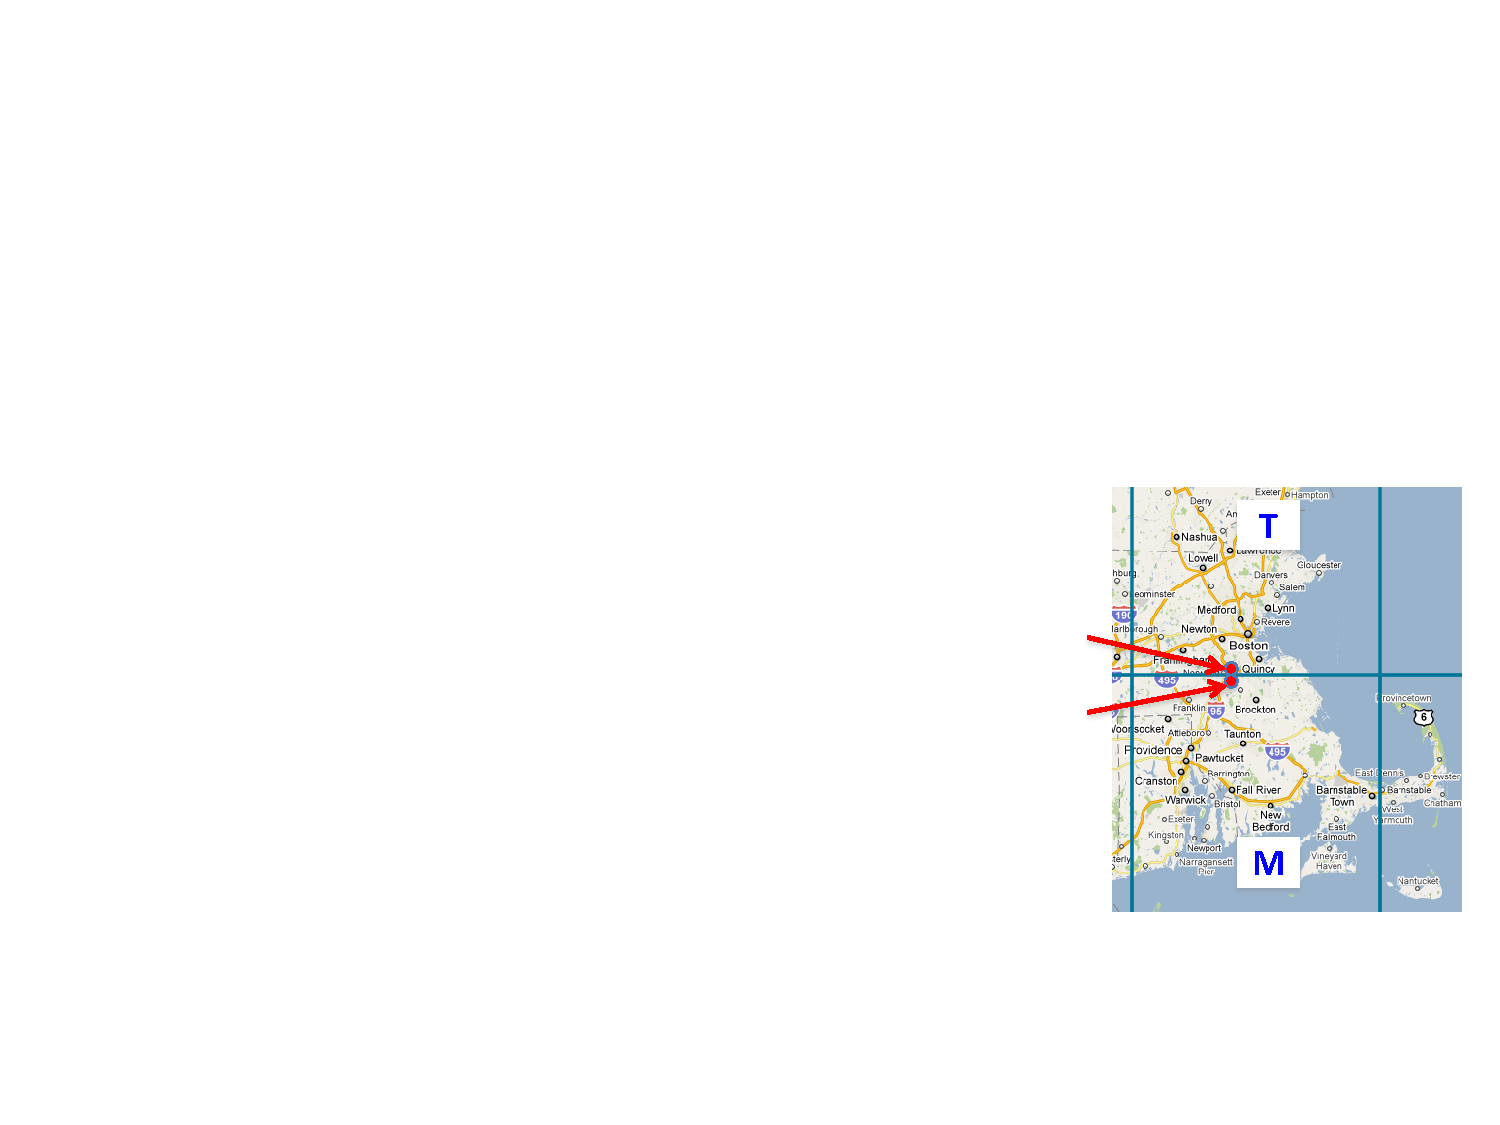
\includegraphics[width=0.7\textwidth]{figures/geohash_edges.pdf}
    \caption{Geohash edge case, where two closely positioned points do not share the same Geohash prefix~\cite{Smiley11geohash}.}
    \label{fig:geohash-edge}
  \end{center}
\end{figure}






























%
% foundations - mapping
%

\section{Web Mapping}

Maps have become an almost instinctive way of seeing our world. They probably first appeared over 18,000 years ago and already in the 16th century, they were produced in large numbers for navigational and military purposes. Maps are powerful tools that help organize boundaries and administrative activities. They allow telling stories, visualizing data and understanding geographic contexts
~\cite{Zzolo11mappingdrupal}.

Recently, Google Maps\footnote{\url{http://maps.google.com}} has made digital maps available to a large number of internet users. \textit{Digital natives} are used to navigate by using interactive maps on their smart phones and look up places on online maps on their computers.

Web mapping describes the whole process of designing, implementing, generating and delivering maps on the internet. It applies theoretical foundations from web cartography to the technical possibilities and boundaries of constantly evolving web technologies. The continuous development of related technologies has created a wide variety of \textit{types of web maps}: from analytic, animated, collaborative and dynamically created web maps to online atlases, realtime and static web maps~\cite{wiki:web-mapping}.

In order to represent spatial locations, \textit{reference systems} are used, that subdivide the geographic area into units of common shape and size. Such spatial reference systems consist of a \textit{coordinate system}, a \textit{datum} and a \textit{projection}. \textit{Geodetic datums} are models that approximate the shape of the Earth. In the following two chapters, the remaining concepts of coordinate systems and map projections will be explained in more detail.

\subsection{Coordinate systems}
\label{chapter:coordinates}

In mapping, a coordinate system is used to represent spatial locations in a numeric way. We mainly differentiate between \textit{Cartesian} and \textit{Ellipsoidal} coordinate systems. 

\begin{itemize}

\item \textbf{Cartesian coordinate systems} express a spatial location by specifying the distances from a point of origin on axes. The axes are usually labeled $X$, $Y$ and $Z$ for locations in three-dimensional space. As an example, the \textit{Earth Centered, Earth Fixed X, Y, and Z (ECEF)} coordinate system is used by positioning technologies such as GPS. The coordinates of New York in ECEF are:

\[ (X, Y, Z) = (1334.409~km, -4653.636~km, 4138.626~km) \]

``Earth centered'' emphasizes that the origin of the axes is defined to be at the geocenter of the planet. For many tasks, this system isn't intuitive as the values don't indicate, if a location is on, above or below the surface of the Earth. 

\item \textbf{Ellipsoidal coordinate systems} describe a more convenient way of expressing spatial location on the Earth's surface. A \textit{reference ellipsoid} approximates the shape of the Earth by an equatorial and a polar radius. As a result, positions at the surface of the Earth can be represented as angles. This defines the primary way of expressing coordinates as a pair of \textit{latitude} and \textit{longitude} values.

  \begin{itemize}

  \item \textbf{Latitude} classifies the angular distance towards north and south from the equator which is at $0^\circ$. Positive latitude values represent the northern hemisphere up the the pole at $90^\circ$. Negative values are located below the equator where the south pole marks the lower limit at $-90^\circ$.

  \item \textbf{Longitude} denotes the angular distance towards west and east. It's zero-mark is a latitude of $0^\circ$,  which runs north-south through the Royal Observatory at Greenwich in the UK. In contrast to latitude values, the longitude encloses a whole circle around the earth. Negative values down to $-180^\circ$ are located west and positive values up to $180^\circ$ are positioned east of Greenwhich.

  \end{itemize}

In classic mapping applications, latitude and longitude values are measured in \textit{degrees, minutes and seconds} of the sphere. New York City is located at $40^\circ$ $43'$ $0''$ North, $74^\circ$ $0'$ $0''$ West. For computational purposes, web mapping is largely based on a \textit{decimal degree} representation of such values. The equivalent decimal degree value for New York in that case is the pair of

  \[ (latitude, longitude) = (40.716667, -74) \]

A common pitfall in web mapping is mixing up the order of latitude and longitude values. Having latitude before longitude is the standard, which means to state the vertical position before the horizontal. This contradicts with classic Cartesian x,y coordinate systems and often leads to confusion. Some mapping APIs expect latitude first, while others are designed to begin with longitude values~\cite{Kupper2005lbs, Zzolo11mappingdrupal}. 

\end{itemize}




\subsection{Map Projections}
\label{chapter:projections}

The planet Earth is a roughly spherical geoid. In order to represent it on flat computer screens, the surface of the Earth needs to be translated to a plane. This is realized by applying the method of a map projection which projects the bended, three-dimensional surface of the Earth onto a two-dimensional projection surface. The shape of the projection surface defines different possibilities of projection types as \textit{planar}, \textit{conical} and \textit{cylindrical}. See figure \ref{fig:map-projection-types} for a visual comparison of map projection types.

\begin{figure}[h]
  \begin{center}
    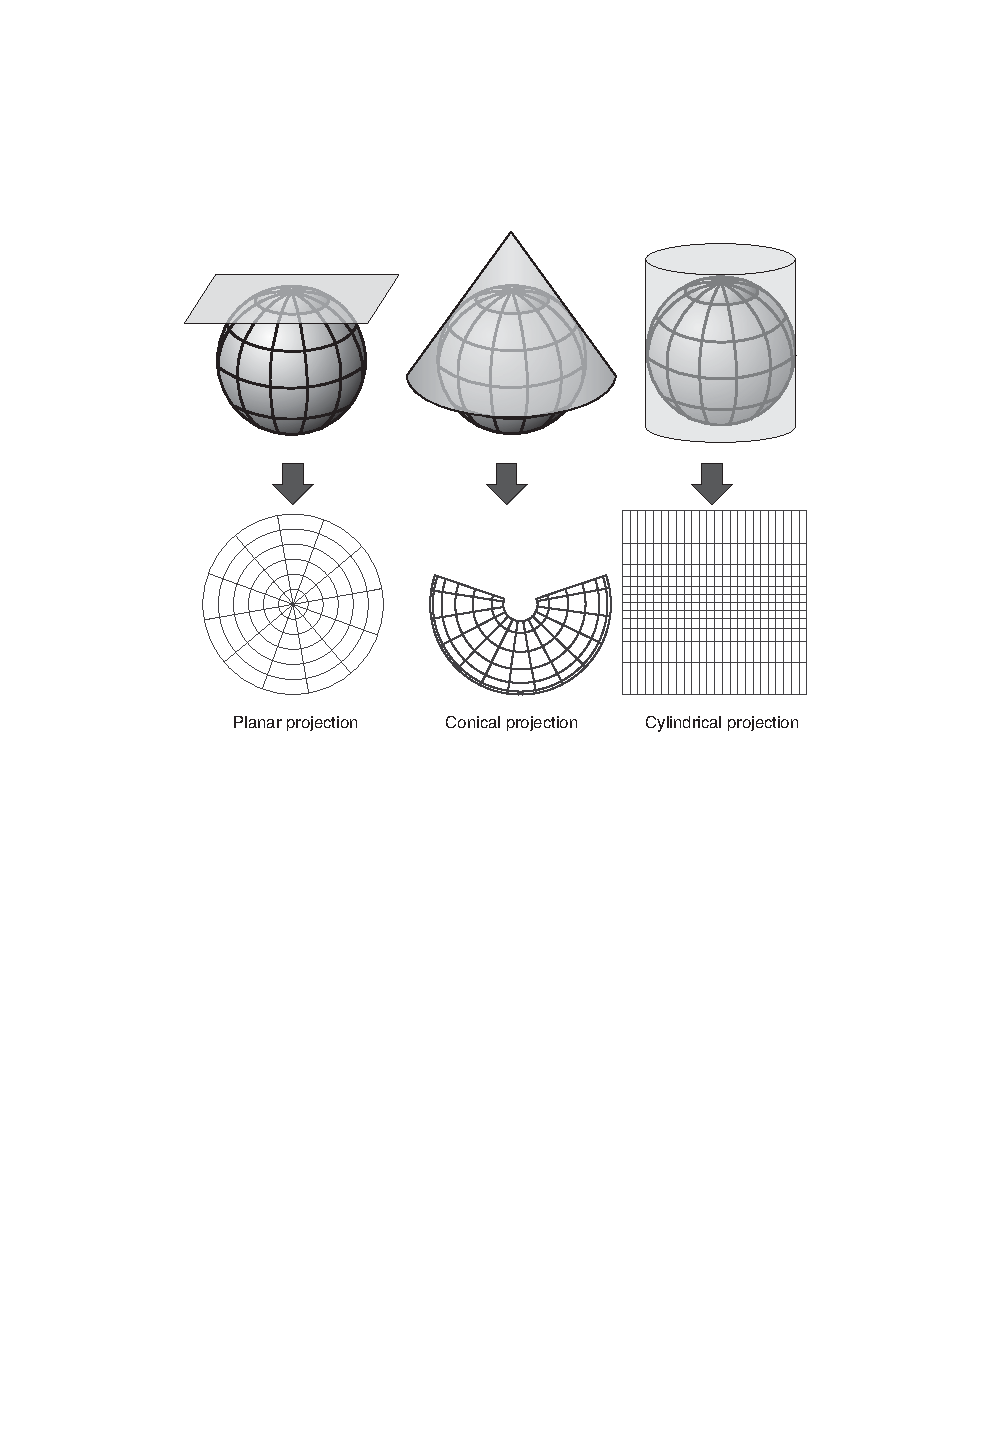
\includegraphics[width=0.75\textwidth]{figures/map_projection_types}
    \caption{Types of map projections~\cite[p 28]{Kupper2005lbs}.}
    \label{fig:map-projection-types}
  \end{center}
\end{figure}

Flattening the curved surface of the Earth naturally causes \textit{distortion} of different kinds, including areal, angular, scale, distance and direction distortion. Selecting a map projection influences which degree and combination of distortion will be caused. As no projection can optimize all those factors at once, choosing the right projection depends on the purpose of the map.

The \textbf{spherical mercator projection} is the most commonly used web mapping projection. Based on a normal cylindrical projection, it preserves local shapes and direction, but does this at the cost of enlarging areas towards the poles. As an example, Greenland appears on a Mercator map larger than South America while its actual size is $1/8$. The effect of this distortion can be visualized by Tissot's indicatrix. Figure \ref{fig:mercator} shows how circles of the same relative size get extrapolated towards the poles when using the mercator projection~\cite{Zzolo11mappingdrupal, wiki:web-mapping, Kupper2005lbs}. 

\begin{figure}[h]
  \begin{center}
    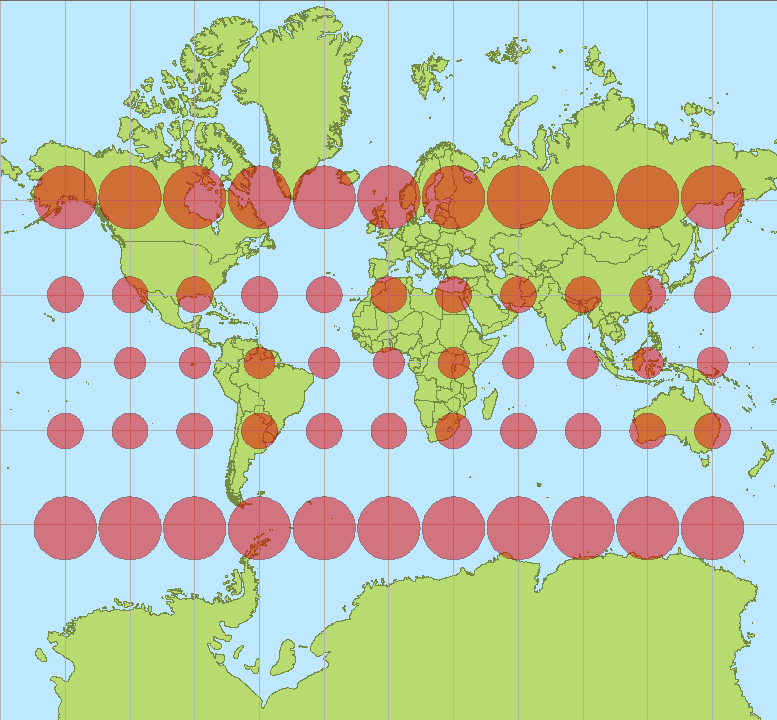
\includegraphics[width=0.65\textwidth]{figures/tissot_mercator.png}
    \caption{Tissot's indicatrix visualizes enlarged areas towards the poles when using the mercator projection~\cite{wiki:mercator}.}
    \label{fig:mercator}
  \end{center}
\end{figure}

Many countries have developed their own coordinate systems, such as the British National Grid or the German Gau\ss-Kr\"{u}ger coordinate system. They aim at reproducing the geographic regions within their territory in an appropriate manner. Standardization efforts go towards using the \textit{Universal Transverse Mercator} projection. It avoids large distortions by comprising a series of Transversal Mercator projections that create separate grid zones with their own projections. This has the benefit of universally representing areas in a more exact way. On the other hand, coordinates need to be referenced including the zones in which they are located in~\cite{Kupper2005lbs}.

\subsection{Spatial data types}

Two main representation types for spatial objects such as buildings, roads and other geometries exist: \textit{vector data} and \textit{raster data}. This mainly applies to 2-dimensional representation of spatial data, which often suffices the task for creating web maps and is preferred over 3-dimensional data handling in many cases for computational simplicity. Figure \ref{fig:raster-vector} illustrates the conceptual different between both data types which will be discussed as follows.

\begin{figure}[h]
  \begin{center}
    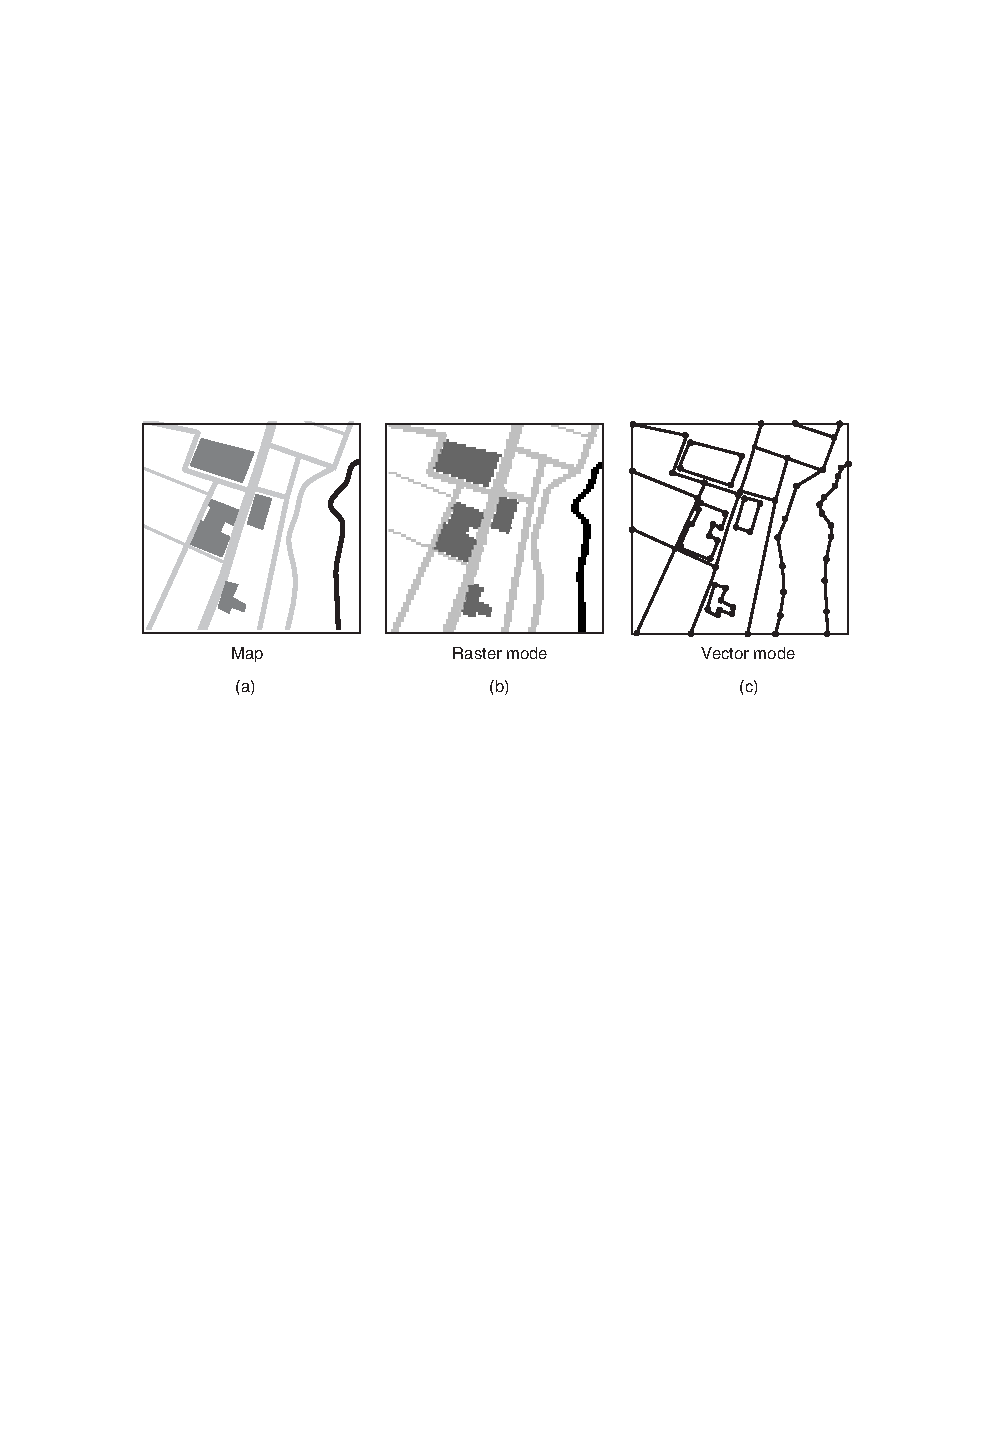
\includegraphics[width=0.9\textwidth]{figures/raster_vs_vector.pdf}
    \caption{A map (a) displayed either in raster mode (b) or in vector mode (c)~\cite[page~38]{Kupper2005lbs}.}
    \label{fig:raster-vector}
  \end{center}
\end{figure}

\begin{itemize}

\item \textbf{Vector data} is used to describe geometric shapes in a numeric way. \textit{Points}, \textit{lines} or \textit{polygons} are specified by coordinates in a reference system.

Simple points can be easily expressed as pairs of latitude, longitude values and stored within two separate columns within a database. More complex shapes like polygons require different data storage types, such as \textit{Well Known Text} (WKT) or \textit{Keyhole Markup Language} (KML).

\item \textbf{Raster data} represents and stores geospatial data as a grid of pixels that forms a continuos surface. It is most commonly used for satellite imaginary. The arrangement of adjacent pixels intrinsically defines the spatial location of shapes within the raster image in relation to an externally defined reference system.

The pixel values of the raster image usually depict a visual representation of the contained area, but they can also be assigned a specific meaning: The \textit{digital elevation model} (DEM) for example is used to describe the average elevation of the mapped area on a per-pixel-basis. Raster images are also often generated from vector data by a tile renderer to create base layers for maps~\cite{Kupper2005lbs, Zzolo11mappingdrupal}.

\end{itemize}







TODO: outro



%
% state of the art
%

\chapter{State of the Art}
\label{chapter:state}

The following chapter discusses the state of the art of related technologies for the thesis. A modern web mapping stack is explained as well as the basics of Drupal \& mapping technologies. Further, the state of the art for client-side and server-side clustering technologies in web mapping will be analyzed.


%
% foundations - mapping
%

\section{A Modern Web Mapping Stack}

The primary purpose of web mapping applications is to deliver spatial data in the form of a map to the user. Modern, interactive web mapping applications are based on a concept named \textit{slippy maps}. These maps are brought to the user by a combination of client- and server-side technologies. Figure \ref{fig:web-mapping-stack} illustrates the prototype of such a modern web mapping application. Similar mapping stacks are documented in 
\cite{Schuetze07smart, mitchell2008web, Miler10webis, McArdle10arch}. Its components will be discussed in the following section.


\begin{figure}[h]
  \begin{center}
    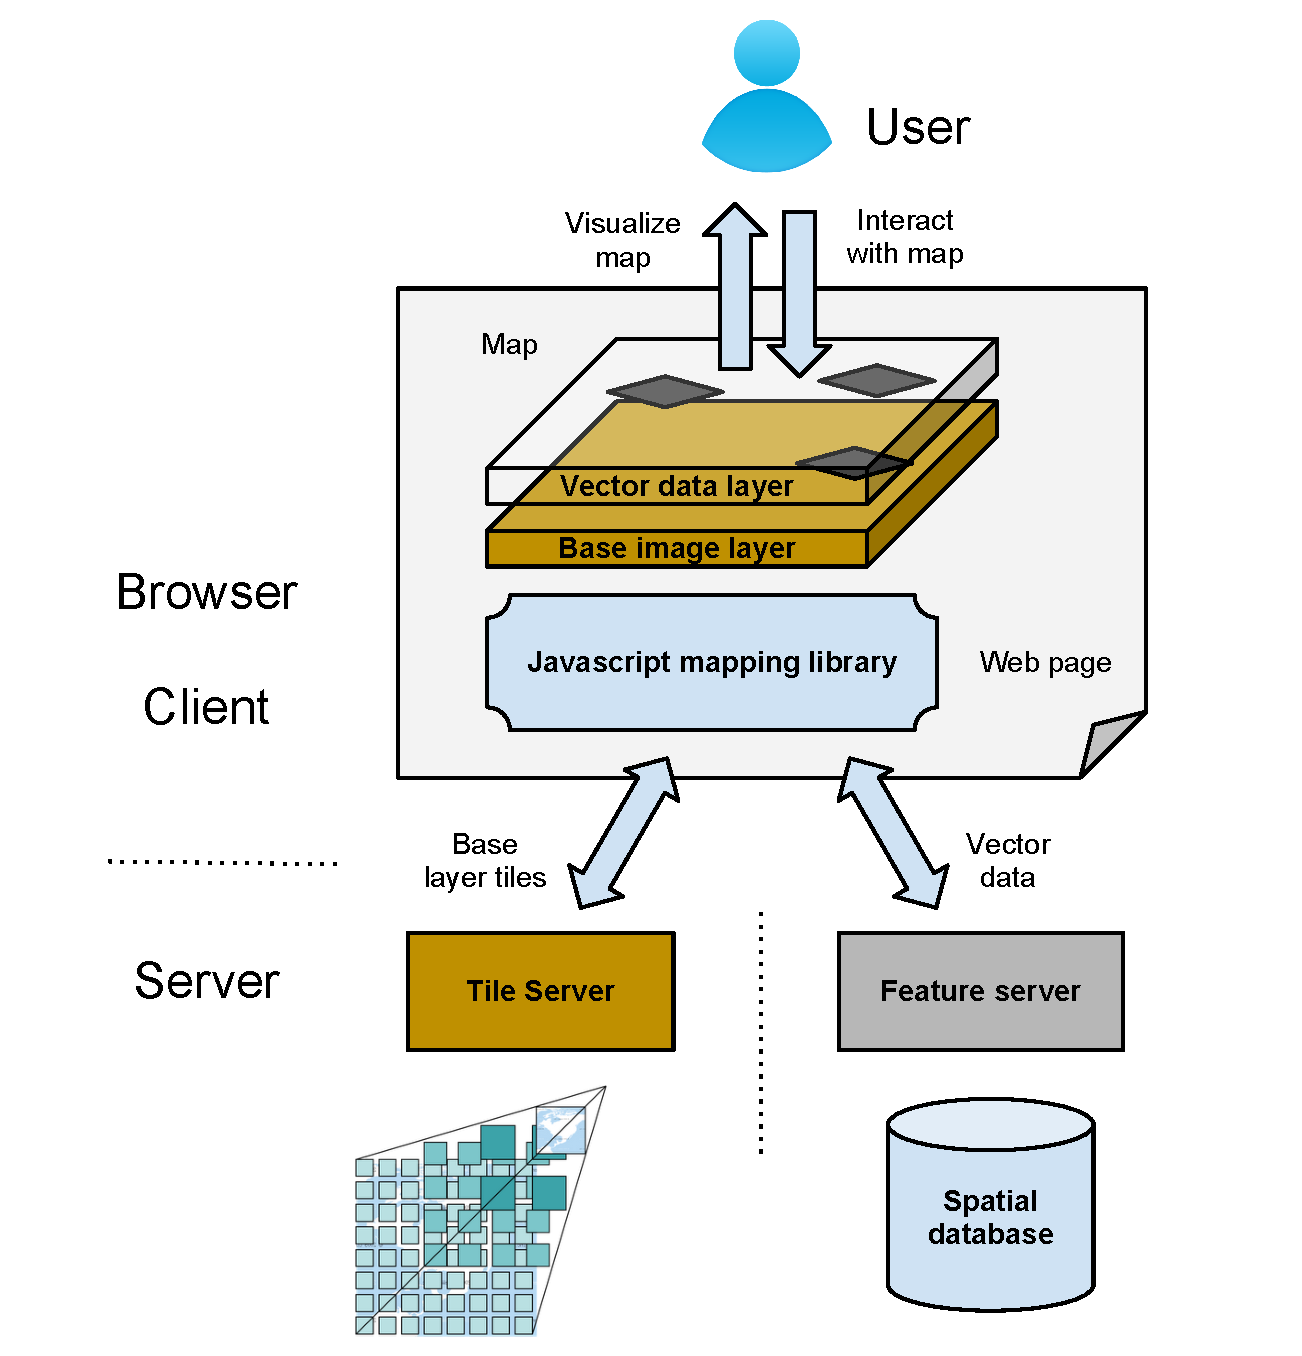
\includegraphics[width=1\textwidth]{figures/web_mapping_stack.pdf}
    \caption{Illustration of a modern web mapping application. Includes a tile graphic from~\cite{web:cubeservtiles}.}
    \label{fig:web-mapping-stack}
  \end{center}
\end{figure}


\begin{itemize}

\item A \textbf{slippy map} is displayed to the user in a rectangular viewport within the browser and handled by a JavaScript mapping library. The map is visualized dynamically by rendering layers of raster and vector data on top of each other. In addition, the slippy map provides means of interaction to the user such as panning and zooming to update and explore the map. 

\item A \textbf{JavaScript mapping library} is in charge of rendering the slippy map by positioning one or multiple layers on top of each other. Usually, a base layer of raster data is combined with a vector data layer on top of it.

Current JavaScript mapping libraries include \textit{OpenLayers}\footnote{\url{http://openlayers.org/}}, \textit{Leaflet}\footnote{\url{http://leafletjs.com/}} and \textit{Modest Maps}\footnote{\url{http://modestmaps.com/}}.

\item A \textbf{tile server} provides static, sliced-up images of the raster image data which the JavaScript mapping library requests on demand, based on the current viewport. When the users performs actions like dragging and zooming on the map, the current viewport will get changed. The JavaScript library then requests additional data from the server if needed and updates the map accordingly. This live-updating process is also referred to as \textit{Bounding Box Strategy} (BBOX Strategy)\footnote{\url{http://openlayers.org/dev/examples/strategy-bbox.html}}. Standards for consuming tiles include \textit{Web Map Service} (WMS)\footnote{\url{http://en.wikipedia.org/wiki/Web_Map_Service}} and \textit{Tile Map Service} (TMS)\footnote{\url{http://en.wikipedia.org/wiki/Tile_Map_Service}}.

A typical tile set represents $256 \times 256$ pixel tiles of the whole world at 18 zoom levels. The fact that this leads to billions of tiles has created its own line of businesses including \textit{Google Maps}\footnote{\url{http://maps.google.com/}}, \textit{Stamen}\footnote{\url{http://maps.stamen.com/}} and \textit{MapBox}\footnote{\url{http://mapbox.com//}}.

\item A \textbf{feature server} provides vector data to the JavaScript mapping library in an analogous way as the tile server does. Note the difference: while raster data will be displayed directly as an image, the vector data gets rendered on the client-side.

To provide dynamic data, the feature server usually relies on a \textit{spatial database}. Spatial extensions exist for various databases, including \textit{PostGis}\footnote{\url{http://en.wikipedia.org/wiki/PostGIS}} and \textit{MySQL Spatial Extensions}\footnote{\url{http://dev.mysql.com/doc/refman/5.0/en/spatial-extensions.html}} and \textit{Spatialite}\footnote{\url{http://www.gaia-gis.it/gaia-sins/}}.

\end{itemize}













%
% state - drupal mapping
%

\section{Drupal \& Mapping}
\label{chapter:drupal-mapping}

As the web, Drupal is a constantly evolving platform. The book ``Mapping with Drupal''\cite{Zzolo11mappingdrupal} by Alan Palazzolo and Thomas Turnbull was published in the end of 2011 and gives a throughout overview of available mapping modules for Drupal 7 by that time. Development obviously continued since then, so its a continuous exercise to keep up-to-date with recent technologies.

\subsection{Data storage}

The \textbf{Geofield}\footnote{\url{http://drupal.org/project/geofield}} module is stated to be the ``best choice for all but the simplest mapping applications''\cite[page 27]{Zzolo11mappingdrupal} in Drupal 7. By using the \textit{geoPHP library}\footnote{\url{https://github.com/phayes/geoPHP}} for geometry operations it allows to store location data in various formats as latitude/longitude, WKT. It integrates with various other mapping modules related to data input and storage in Drupal, as illustrated in figure \ref{fig:geofield}.

\begin{figure}[h]
  \begin{center}
    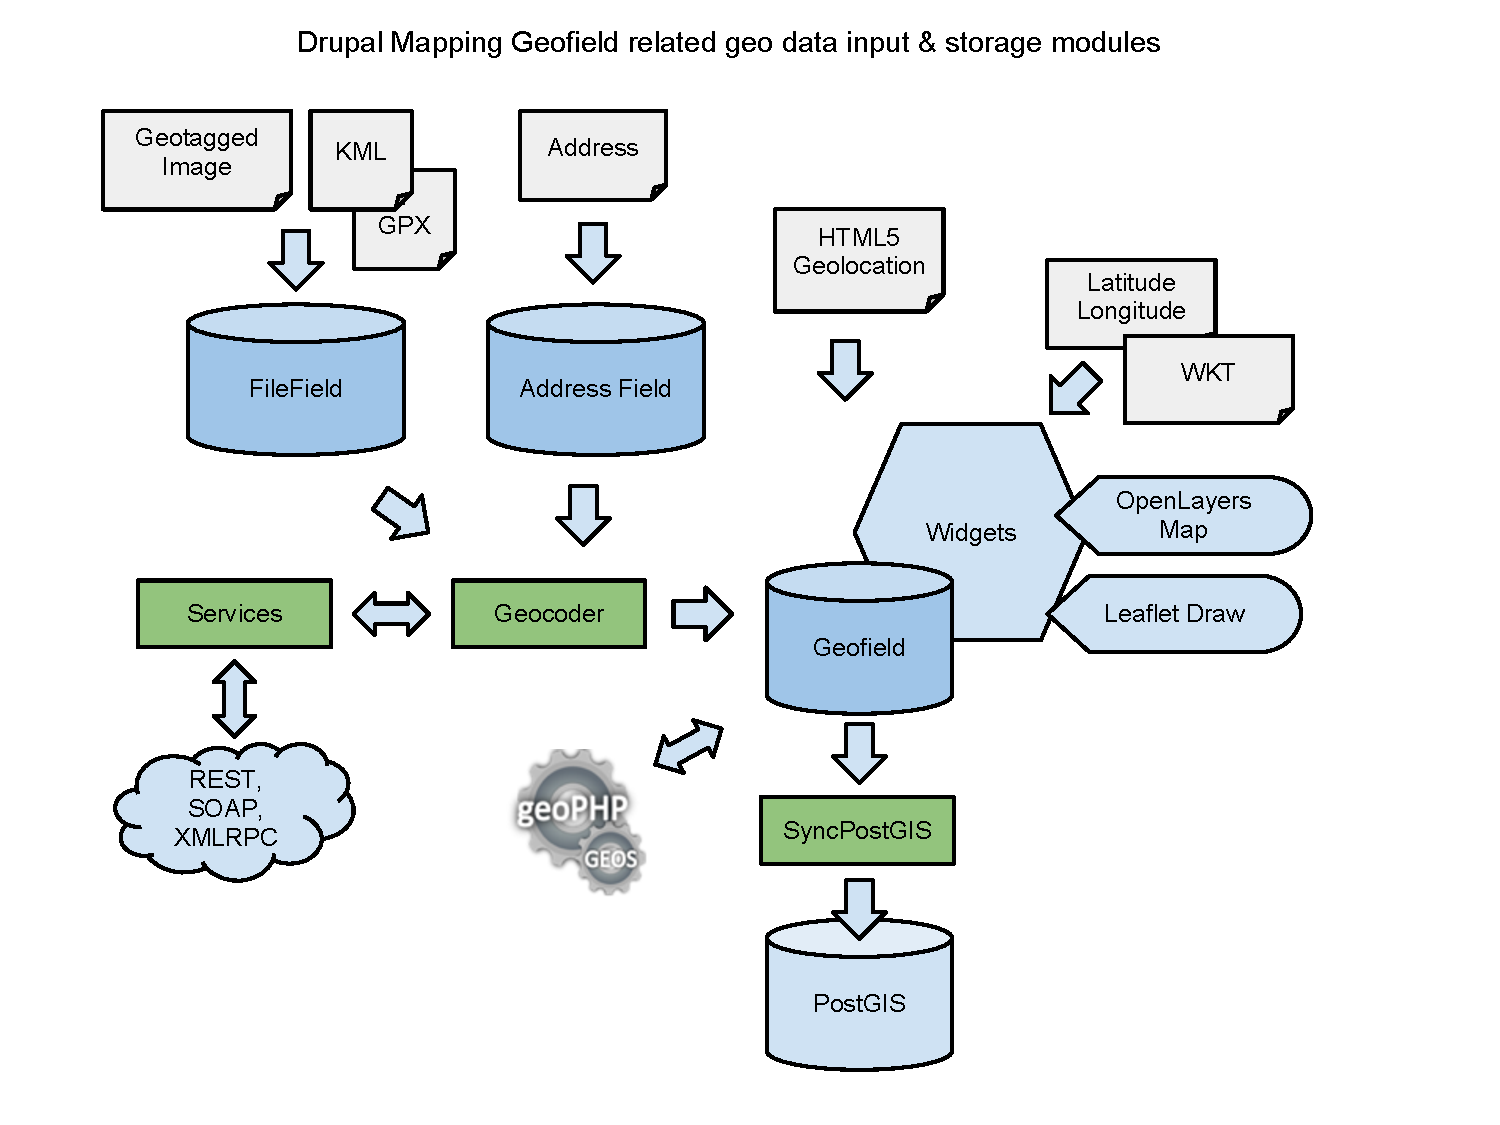
\includegraphics[width=1.2\textwidth]{figures/drupal_mapping_geofield.pdf}
    \caption{The Drupal Geofield module and related geo data input and storage modules.}
    \label{fig:geofield}
  \end{center}
\end{figure}

Besides the geofield module, the following modules are relevant to its main task of storing location data: 

\begin{itemize}

\item \textbf{PostGIS integration} is often requested when dealing with complex spatial data. A variety of modules and approaches exist for integration with PostGIS. The \textit{PostGIS} module\footnote{\url{http://drupal.org/project/postgis}} is similar to Geofield but relies on PostGIS for spatial operations and data storage. \textit{Sync PostGIS}\footnote{\url{http://drupal.org/project/sync_postgis}} allows to push geospatial data from a Drupal-internal storage as Geofield into PostGIS. Recently, a pluggable storage backend was added\footnote{\url{http://drupal.org/node/1728530}} to the Geofield module in order to allow integration with alternative databases. \textit{Geofield PostGIS}\footnote{\url{https://github.com/phayes/geofield_postgis}} therefore is a more integrated option for storing Geofield data in PostGIS.

\item \textbf{Solr integration} is another common approach when creating maps based on Drupal. \textit{Apache Solr search} is a fast open source search platform written in the Java programming language. There are two common modules for Solr integration in Drupal which both offer support for indexing spatial data: \textit{Search API}\footnote{\url{http://drupal.org/project/search_api}} and \textit{Apache Solr Search Integration}\footnote{\url{http://drupal.org/project/apachesolr}}.

\item The \textbf{Location}\footnote{\url{http://drupal.org/project/location}} module is another popular choice for storing spatial data in Drupal 7. As its architecture doesn't follow current Drupal conventions, its rather a monolithic system that provides a rich out-of-the-box experience but doesn't integrate that well with other modules like Geofield does~\cite{Zzolo11mappingdrupal}.

\end{itemize}

\subsection{Data presentation}

Being a content management system and framework, the second most important task for handling spatial data in Drupal is presenting it in various ways. Again, a variety of modules exists for querying and displaying geospatial data. Figure \ref{fig:drupal-mapping-display} illustrates how the query- and display-related Drupal mapping modules work together in a common use case.

A \textbf{mapping module} provides the basic integration a JavaScript mapping library with the Drupal internals. The most widely used mapping modules are the \textit{OpenLayers} module\footnote{\url{http://drupal.org/project/openlayers}} with 7,205 active installations on Drupal 7 by January 2012 and the GMap module\footnote{\url{http://drupal.org/project/gmap}} with 21,920. The Leaflet module\footnote{\url{http://drupal.org/project/leaflet}} only counts 496 active installations reported by drupal.org by that time, but has the advantage of being more lightweight than OpenLayers and is not bound to a single, commercial API as GMap.

\begin{figure}[h]
  \begin{center}
    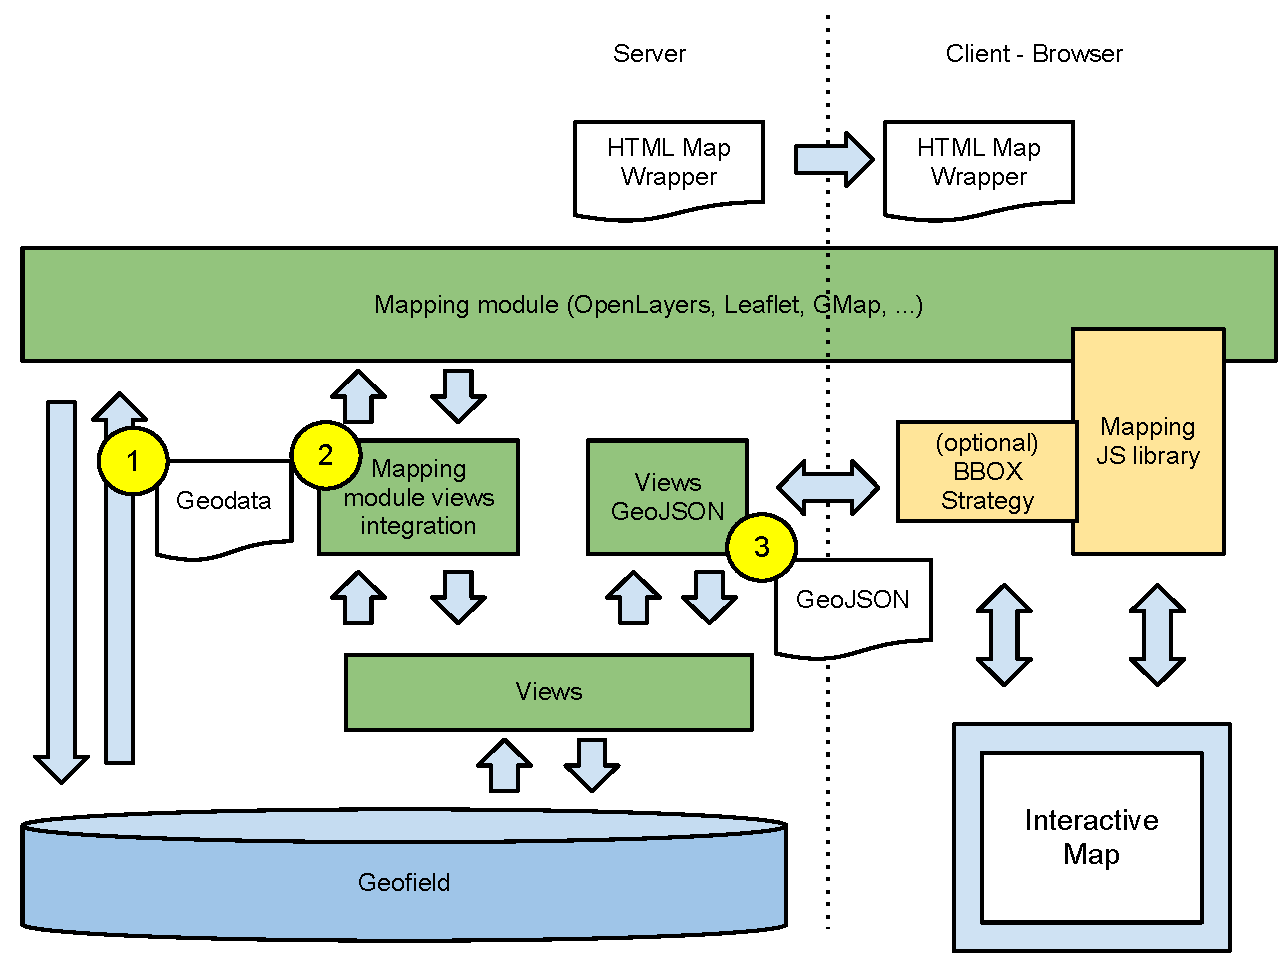
\includegraphics[width=1\textwidth]{figures/drupal_mapping_display.pdf}
    \caption{The prototypic work-flow of query and display-related Drupal mapping modules.}
    \label{fig:drupal-mapping-display}
  \end{center}
\end{figure}

The interaction with the spatial data provided by the Geofield module can be classified into three different scenario types, visualized by circles within figure \ref{fig:drupal-mapping-display}:

\begin{enumerate}

\item In the first scenario, the mapping module directly accesses data from Geofield. This approach is usually applied when displaying maps with single location items. The geodata retrieved from Geofield is then transferred to the client within the HTML response. On the client-side, the JavaScript mapping library takes care of visualizing the geodata.

\item In the second scenario, integration with the \textbf{Views} module is used to query a collection of data. The Drupal \textit{Views} module\footnote{\url{http://drupal.org/project/views}} is the de-facto standard for creating listings of content of any kind. With 377,956 reported installations by January 2012 it is the most widely used module and it will be part of Drupal 8 core. Integrating with Views allows the mapping module to query a listing of locations from geofield, based user-defined parameters. Instead of returning single locations as in scenario one, the second therefore processes a collection of geodata values. 

\item Scenario three allows for dynamically updating the map based on user interaction. In this case, the geospatial data is not delivered within the HTML response as in the previous approaches. The JavaScript library issues a separate request to the server using a \textbf{Bounding Box strategy}. The OpenLayers JavaScript library contains such a BBOX Strategy\footnote{\url{http://dev.openlayers.org/docs/files/OpenLayers/Strategy/BBOX-js.html}} and the \textit{Leaflet GeoJSON} module\footnote{\url{http://drupal.org/project/leaflet_geojson}} provides the same for the Leaflet library. The strategy essentially requests the geodata within the bounding box of the current viewport. On the server-side, the \textit{Views GeoJSON} module\footnote{\url{http://drupal.org/project/views_geojson}} translates the query and transforms the data returned by Views into a \textit{GeoJSON}\footnote{\url{http://www.geojson.org/}} feed in order to deliver it to the JavaScript mapping library on the client-side.

\end{enumerate}

Note that the exact implementation details vary between the used mapping modules.

\textbf{Solr integration} for querying and displaying geospatial data in Drupal is mainly provided by the integration of the modules with Views. In addition, for the \textit{Apache Solr Search Integration} module exists a \textit{apachesolr\_location} module\footnote{\url{http://drupal.org/project/apachesolr_location}} and a \textit{ApacheSolr Geo} sandbox project\footnote{\url{http://drupal.org/sandbox/pwolanin/1497066}}. For \textit{Search API} there is a \textit{Search API Location}\footnote{\url{http://drupal.org/project/search_api_location}} module.





%
% state - mapping stack
%

\section{Clustering implementations in Web Mapping}

Clustering in web mapping affects the way how vector data is processed and represented to the user.  According to the web mapping stack described in \ref{chapter:web-mapping-stack}, we can differentiate between client-side and server-side clustering. A server-side clustering implementation will cluster the data already before sending it over the network to the browser client. In a client-side clustering implementation, the client receives the unclustered data set from the server and clusters it on its own.

\textbf{Client-side vs. server-side clustering}

Client-side clustering is convenient because of several reasons. The clustering task can be abstracted from the server without the need to account for server-side implementation details. It also relieves the server from performing the clustering task which can positively influence scalability. Executing the clustering task on the client-side allows for better interaction: the user may zoom into or expand clusters without the need for an additional request to the server. 

On the other hand, client-side clustering forces the server to deliver the entire data set. This also means that a bigger amount of data has to be processed and transferred over the network. Subsequently, the client needs to cope with receiving the larger data set and takes over the burden of clustering the data.

\subsection{Client-side clustering in Web Mapping}

When clustering on the client-side, the JavaScript mapping library receives the entire, unclustered data set and executes a clustering algorithm before visualizing the data to the user.

\begin{itemize}

\item The \textbf{Leaflet.markercluster}\footnote{\url{https://github.com/Leaflet/Leaflet.markercluster/}} library provides animated marker clustering for the Leaflet JavaScript mapping library. It combines the \textit{agglomerative hierarchical clustering algorithm} with a \textit{distance grid} (see chapters \ref{chapter:clustering-hierarchical} and \ref{chapter:clustering-grid}). The library features advanced cluster visualization techniques for representing shapes of clustered items and animations. When the user zooms into the map, clusters get expanded in a visual way and they collapse in the opposite direction.

Leaflet.markercluster leverages the advantages of being a client-side implementation by implementing a \textit{hierarchical clustering} approach that precalculates the clusters for all zoom levels. The markers are inserted into a distance grid on the lowest zoom level. The grid is then used to check for overlapping neighbors. If the inserted marker needs to get merged, this information is automatically propagated to upper levels within the hierarchy. Otherwise, the same checking procedure will be repeated for the inserted marker on the next, upper level.

The cluster visualization of Leaflet.markercluster is supported by the \textit{QuickHull}\footnote{\url{http://en.wikipedia.org/wiki/QuickHull/}} algorithm to compute the enclosing \textit{convex hull} of the clustered points as illustrated in b) of figure \ref{fig:leaflet}. In addition, a \textit{spiderfier} algorithm allows the user to select clustered points, even if they are positioned very closely to each other, see a) in figure \ref{fig:leaflet}.

The clustering task is computed in \textit{linear time} to the number of markers $n$ and the usually constant number of zoom levels. 

\begin{figure}[h]
  \begin{center}
    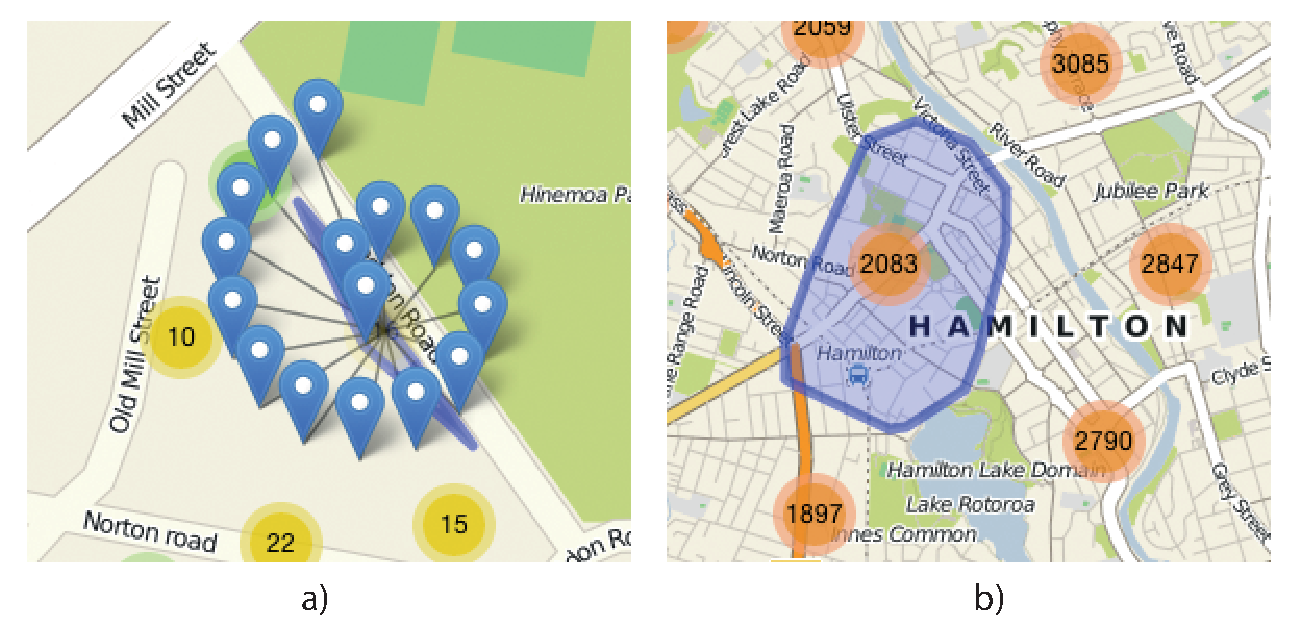
\includegraphics[width=1\textwidth]{figures/leaflet.pdf}
    \caption{Two screenshots taken from the Leaflet.markercluster example map: a) spiderfied representation to select from multiple overlapping points and b) the visualized convex hull of a cluster indicates the real shape of the cluster on mouse-hover.}
    \label{fig:leaflet}
  \end{center}
\end{figure}

\item The \textbf{OpenLayers Cluster Strategy}\footnote{\url{http://dev.openlayers.org/releases/OpenLayers-2.12/lib/OpenLayers/Strategy/Cluster.js}} is included in the OpenLayers library and provides a simple \textit{distance-based}, client-side clustering.

When creating the clustering, the features are sequentially inserted. Every new feature is compared against all existing clusters. If the new feature overlaps with any cluster, it will get merged into the existing cluster. Otherwise, the feature is inserted as its own cluster. Once the data, viewport or zoom level changes, the clustering process will be re-initiated. 

The sequential insertion and the comparison to all existing clusters leads to a \textit{factorial time complexity} of the algorithm. 

\item \textbf{k-means clustering}\footnote{\url{http://polymaps.org/ex/kmeans.js}} is a clustering library for the \textit{Polymaps} JavaScript mapping library. It leverages the k-means squared error algorithm discussed in chapter \ref{chapter:k-means} to create clusters in linear time. As discussed, the k-means algorithm computes in \textit{linear time}.

\end{itemize}

Other client-side clustering libraries evaluated can be classified similarly to the previously discussed ones. Grid-based approaches similar to Leaflet.markercluster include the Clustr library\footnote{\url{https://github.com/mapbox/clustr}} for Modest Maps and Clusterer2\footnote{\url{http://www.acme.com/javascript/\#Clusterer}} for Google Maps. MarkerClustererPlus for Google Maps V3\footnote{\url{http://code.google.com/p/google-maps-utility-library-v3/wiki/Libraries\#MarkerClusterer}} takes an approach similar to the OpenLayers Cluster Strategy.

\subsection{Server-side clustering in Web Mapping}

Server-side implementations cluster the data already before sending it over the network to the client.

While client-side clustering solutions are standardized towards available JavaScript mapping libraries, this doesn't apply to server-side implementations. Clustering on the server-side can be performed both on the database and/or application layer. The wide variety of tools involved in the server-side mapping stack from different spatial databases and programming languages seems to make it harder to establish off-the-shelf libraries for server-side clustering, as they always need to be integrated into a certain architecture.

\begin{itemize}

\item \textbf{Clustering maps} by Wannes Meert is the only scientific publication found that explores server-side clustering for web mapping. The study compares strengths and weaknesses of three different approaches (\textit{K-means}, \textit{Hierarichal clustering} and \textit{DBSCAN}) and finally implements density-based clustering. The solution is based on the \textit{DBSCAN} algorithm and uses the \text{R-tree} as indexing structure to speed up neighborhood searches. It is implemented and documented as a \textit{PHP server-side script}. The time complexity of the implemented and discussed final algorithm is quasilinear: $\BigO{n \log{n}}$ and the demonstration page\footnote{\url{http://www.wannesm.be/maps/}} asserts a clustering time of $\sim 1$ second for only 525 points~\cite{Meert06clustermaps}.

\item \textbf{Google Maps Hacks: Tips and Tools for Geographic Searching and Remixing} is a book that contains a section \textit{Hack 69. Cluster Markers at High Zoom Levels} that discussed various approaches to server-side cluster markers for Google Maps. The chapter evaluates different approaches from a quadratic-time $\BigO{n^2}$ implementation of the \textit{k-means} algorithm over a even worse cubic-time $\BigO{n^3}$, \textit{hierarchical clustering} approach. Finally, a \textit{naive grid-based clustering} solution is developed and documented as a \textit{CGI Perl Script} which is stated to perform in linear time $\BigO{n}$~\cite{Gibson06Gmapshacks}.

\item \textbf{Geoclustering}\footnote{\url{https://github.com/ahtih/Geoclustering}} is a Drupal 6 module designed to ``scale to 100 000+ markers''. By maintaining a cluster tree in a separate database table, it essentially pre-calculates clusters. Similar to the grid-based clustering algorithm \textit{STING} described in \ref{chapter:clustering-grid}, by shifting the clustering complexity to the calculation of the cluster tree, queries can be performed in constant time, only linear to the number of grids $\BigO{g}$. This speed improvement reduces the possibilities of dynamic filtering to bounding-box filters only. Filters on other properties of the indexed data would need to be pre-calculated into a more complex or separate cluster trees.

\item \textbf{Clustering in Apache Solr} has been researched as well. While Solr integrates Carrot2 as a document clustering engine\footnote{\url{http://searchhub.org/2009/09/28/solrs-new-clustering-capabilities/}}, spatial clustering isn't supported out-of-the-box. A tutorial written in German documents the conceptual implementation of grid-based clustering in Solr\footnote{\url{http://blog.sybit.de/2010/11/geografische-suche-mit-solr/}}. As Geohash support has been added to Solr to support proximity searches~\cite{Smiley11geohash}, it could be used as well for spatially clustering data.  

\end{itemize}


Other server-side clustering implementations have been researched:

On the \textbf{database-layer}, \textit{SQLDM - implementing k-means clustering using SQL} describes a linear-time implementation of the k-means clustering algorithm in \textit{MySQL}\cite{Simha07sqldm}.
 The \textit{PostGIS} spatial extension for the \textit{PostreSQL} database provides grid-based clustering via \textit{ST\_SnapToGrid}\footnote{\url{http://postgis.refractions.net/docs/ST_SnapToGrid.html}}. Also, a k-means module\footnote{\url{http://pgxn.org/dist/kmeans/doc/kmeans.html}} (also see \footnote{\url{http://gis.stackexchange.com/questions/11567/spatial-clustering-with-postgis}}) and documentation for clustering indices based on \textit{Geohash} \footnote{\url{http://workshops.opengeo.org/postgis-intro/clusterindex.html\#clustering-on-geohash}} for PostGIS exist.

Further, \textbf{application-layer} clustering implementations are grid- and distance-based clustering for Google Maps in PHP\footnote{\url{http://www.appelsiini.net/2008/11/introduction-to-marker-clustering-with-google-maps}}. Vizmo is a research project that developed a server-side clustering component in PHP, Symfony2 and MySQL\footnote{\url{http://www.globalimpactstudy.org/wp-content/uploads/2011/12/vizmo-poster.pdf}}. Beyond the primary scope of PHP applications, a Flex-based clustering implementation has been developed for ArcGIS server\footnote{\url{http://thunderheadxpler.blogspot.co.at/2008/12/clustering-20k-map-points.html}}. ClusterPy\footnote{\url{http://www.rise-group.org/risem/clusterpy/index.html}} is a library of spatially constrained clustering algorithms in Python and SGCS\footnote{\url{http://cran.r-project.org/web/packages/SGCS/}} is a package to build graph based clustering summaries for spatial point patterns in R.
























%
% state - vis
%

\section{Visual mapping}

N\"{o}llenburg~\cite{noellenburg11geovis} names three ``Driving forces in geovisualization'': The advent of high speed parallel processing and technology advances in computer graphics, today allows us to grasp enormous amounts of information. Besides the advances in graphics and display technologies, the second main driving force in geographic visualization is the increasing amount of geospatial data being collected and available. Finally, the third force is the \textit{rise of the Internet}, which significantly pushes web mapping and contributes to geovisualization technologies.

As a logical consequence of broader audiences having access to geospatial visualizations using the Internet, it appears that there is a shift from technology-driven visualization towards more human-centered approaches. Interactive and highly dynamic interfaces have helped the map evolve from its traditional role as a presentational device towards exploring geospatial data~\cite{noellenburg11geovis, vislecture}.

In chapter \ref{chapter:foundations-vis}, foundations of visualization, visual variables and data exploration techniques as well as the concept of clutter reduction have been introduces. In the following, existing visualization techniques for representing clustered data on maps will be discussed. In a first step, visualization concepts on the map level will be discussed. Later, approaches for visualizing individual clusters will are added. 

\subsection{Map visualization types for clustering}
\label{chapter:map-vis}

There exists a variety of map types, serving different purposes like standard geographic maps, cartograms, geologic maps, linguistic maps or weather maps. Some of these use distortion, for example the cartogram can be used to map the area of each country to the size of population. In this section, we try to identify those map types which are appropriate for visualizing clustered data\cite{noellenburg11geovis, wiki:map-types}:

\begin{itemize}

\item \textbf{Geographic map with markers}. The default way of representing data is a standard 2-dimensional map with markers on top of it. Each marker represents a data point or in the case of clustering, a cluster.

\parbox [h]{0.4\textwidth}{
    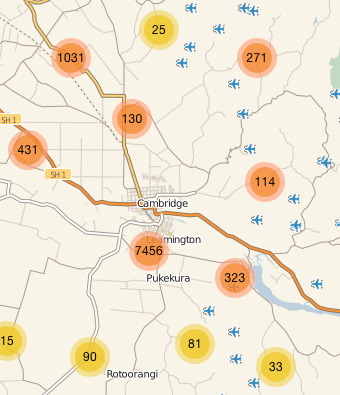
\includegraphics [width=\linewidth]{figures/map_types_normal_leaflet.png}
    \captionof {figure}{Leaflet map}
    \label{fig:map-type-standard-leaflet}
}
\hfill
\hspace{0.5cm}
\parbox [h]{0.4\textwidth }{
    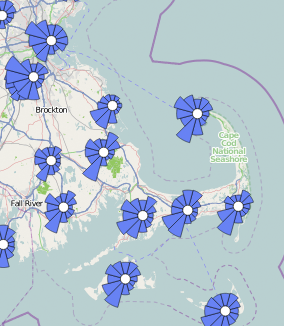
\includegraphics [width=\linewidth]{figures/map_types_standard_wind.png}
    \captionof {figure}{Wind history map}
    \label{fig:map-type-standard-wind}
}

\begin{itemize}

\item Figure \ref{fig:map-type-standard-leaflet} depicts an example\footnote{Leaflet.clustermarker example map from \url{http://leaflet.github.io/Leaflet.markercluster/example/marker-clustering-realworld.10000.html}} of the Leaflet.markercluster library. Clustered results are displayed using markers of the same size. The amount of items within a cluster is indicated by using a ``hot-to-cold'' color ramp~\cite{web:color-ramp}. 

\item Figure \ref{fig:map-type-standard-wind} shows a similar example, in this case a Wind history map\footnote{Wind history map \url{http://windhistory.com/map.html}} with markers for every wind measurement point. In this case, an advanced visualization technique is used for visualizing the amount of wind per cardinal direction as polar area diagrams.

\end {itemize}

The comparison between the two standard maps shows the potential of using advanced visualization techniques for displaying cluster items. Further ways for cluster visualization will be discussed in chapter \ref{chapter:cluster-vis}.

\item \textbf{Geographic Heatmap}

Heatmaps use colored, two-dimensional areas to express the value of each data entity on the map. Choropleth maps are the most common heatmaps, which are often used for analysis of geographic and statistical data. 

\parbox [h]{0.4\textwidth}{
    
\includegraphics [width=\linewidth]{figures/map_types_choropleth.pdf}
    \captionof {figure}{Choropleth map\protect\footnotemark}
    \label{fig:map-type-choropleth}
}\footnotetext{Choropleth map example from Kartograph \url{http://kartograph.org/showcase/choropleth/}}
\hfill
\hspace{0.5cm}
\parbox [h]{0.4\textwidth}{
    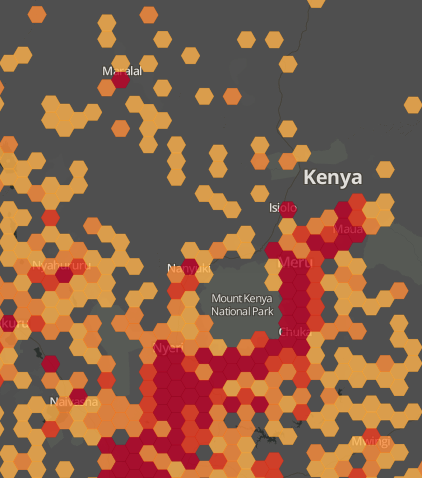
\includegraphics [width=\linewidth]{figures/map_types_heatmap.png}
    \captionof {figure}{Heatmap\protect\footnotemark}
    \label{fig:map-type-binning}
}\footnotetext{Heatmap that uses binning \url{http://mapbox.com/blog/binning-alternative-point-maps/}}


\begin{itemize}

\item Figure \ref{fig:map-type-choropleth} visualizes an example choropleth map that shows population data for each of the departments of metropolean France. Color coding is used to indicate densely populated regions with heavier red tones.

\item Figure \ref{fig:map-type-binning} presents another example that uses \textit{binning} for creating a hexagonal tessellation of the surface in order to visualize clustered results. 

\end {itemize}

A problem with heat maps is that they require a non-overlapping tessellation of the surface to provide the areas for visualization. As the binning example indicates, such a tessellation can also be done programmatically. Heatmap therefore can also be used for visualizating arbitrary clustered data without a need to calculate the exact boundaries of clusters. Another variation of heatmaps is the prism map, which adds extrusion of areas as a third-dimension~\cite{ladenhauf12dia, Delort10vis}. A publication on the evaluation of color schemes in choropleth maps can be found in~\cite{MacEachrenMort}. 


\item \textbf{Dot Grid maps}

Dot Grid maps are based on the suggestion by Jaques Bertin~\cite{bertin67graphics, bertin83graphics} to use graduated sizes in a regular pattern as an alternative to chloropeth maps. The advantage is, that the map creator doesn't have to choose between quantity or density of a distribution value, because the dot grid map shows both a the same time. The user can understand the data distribution on a finer level of granularity, as opposed to where the chloropeth map usually creates larger areas of aggregated information~\cite{web:dot-grid}.

Figure \ref{fig:map-type-dotgrid} is an alternative version of the France map from figure \ref{fig:map-type-choropleth}, visualized as a dot grid map.


\item \textbf{Voronoi map}

The Voronoi tessellation is a space partitioning technique. From a set of points, it produces a Voronoi polygon for each point, such that the area covered is closest to that point in comparison to all other points. Jean-Yves Delort describes a technique that uses Voronoi polygons for ``Vizualizing Large Spatial Datasets in Interactive Maps''~\cite{Delort10vis}. It uses a hierarchical clustering technique to choose a subset of points per zoom level for proper visualization. Still, the effectiveness of this approach is questionable, as the scalability analysis of the studies shows that the technique can efficiently be used for datasets of up to 1000 items.

Figure \ref{fig:map-type-voronoi} show an exemplary voronoi map that displays all U.S. airports as of 2008. Besides the shown visualization, for Voronoi maps apply the same visualization possibilities as for cloropeth maps.

\parbox [h]{0.4\textwidth }{
    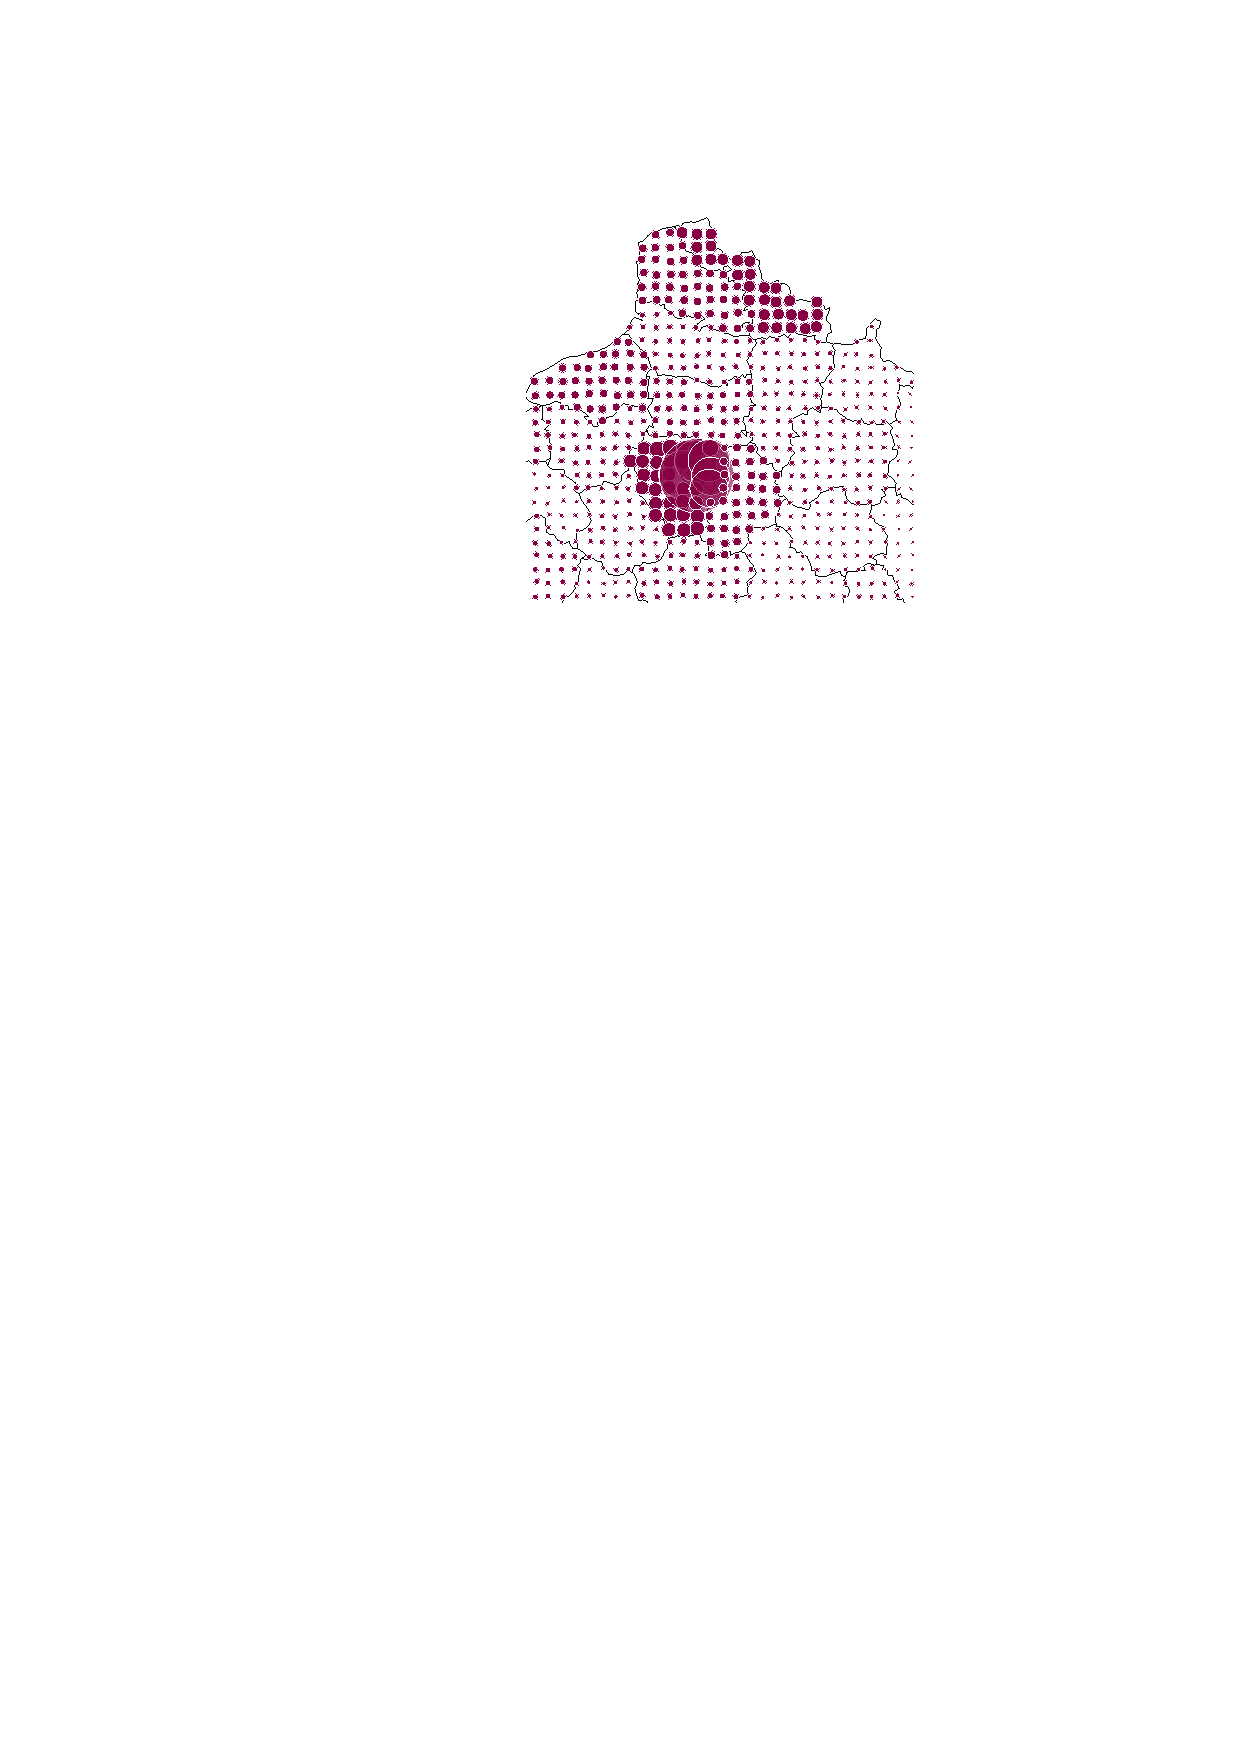
\includegraphics [width=\linewidth]{figures/map_types_dot_grid.pdf}
    \captionof {figure}{Dot Grid map\protect\footnotemark}
    \label{fig:map-type-dotgrid}
}\footnotetext{Dot Grid map example from Kartograph \url{http://kartograph.org/showcase/dotgrid/}}
\hfill
\hspace{0.5cm}
\parbox [h]{0.4\textwidth }{
    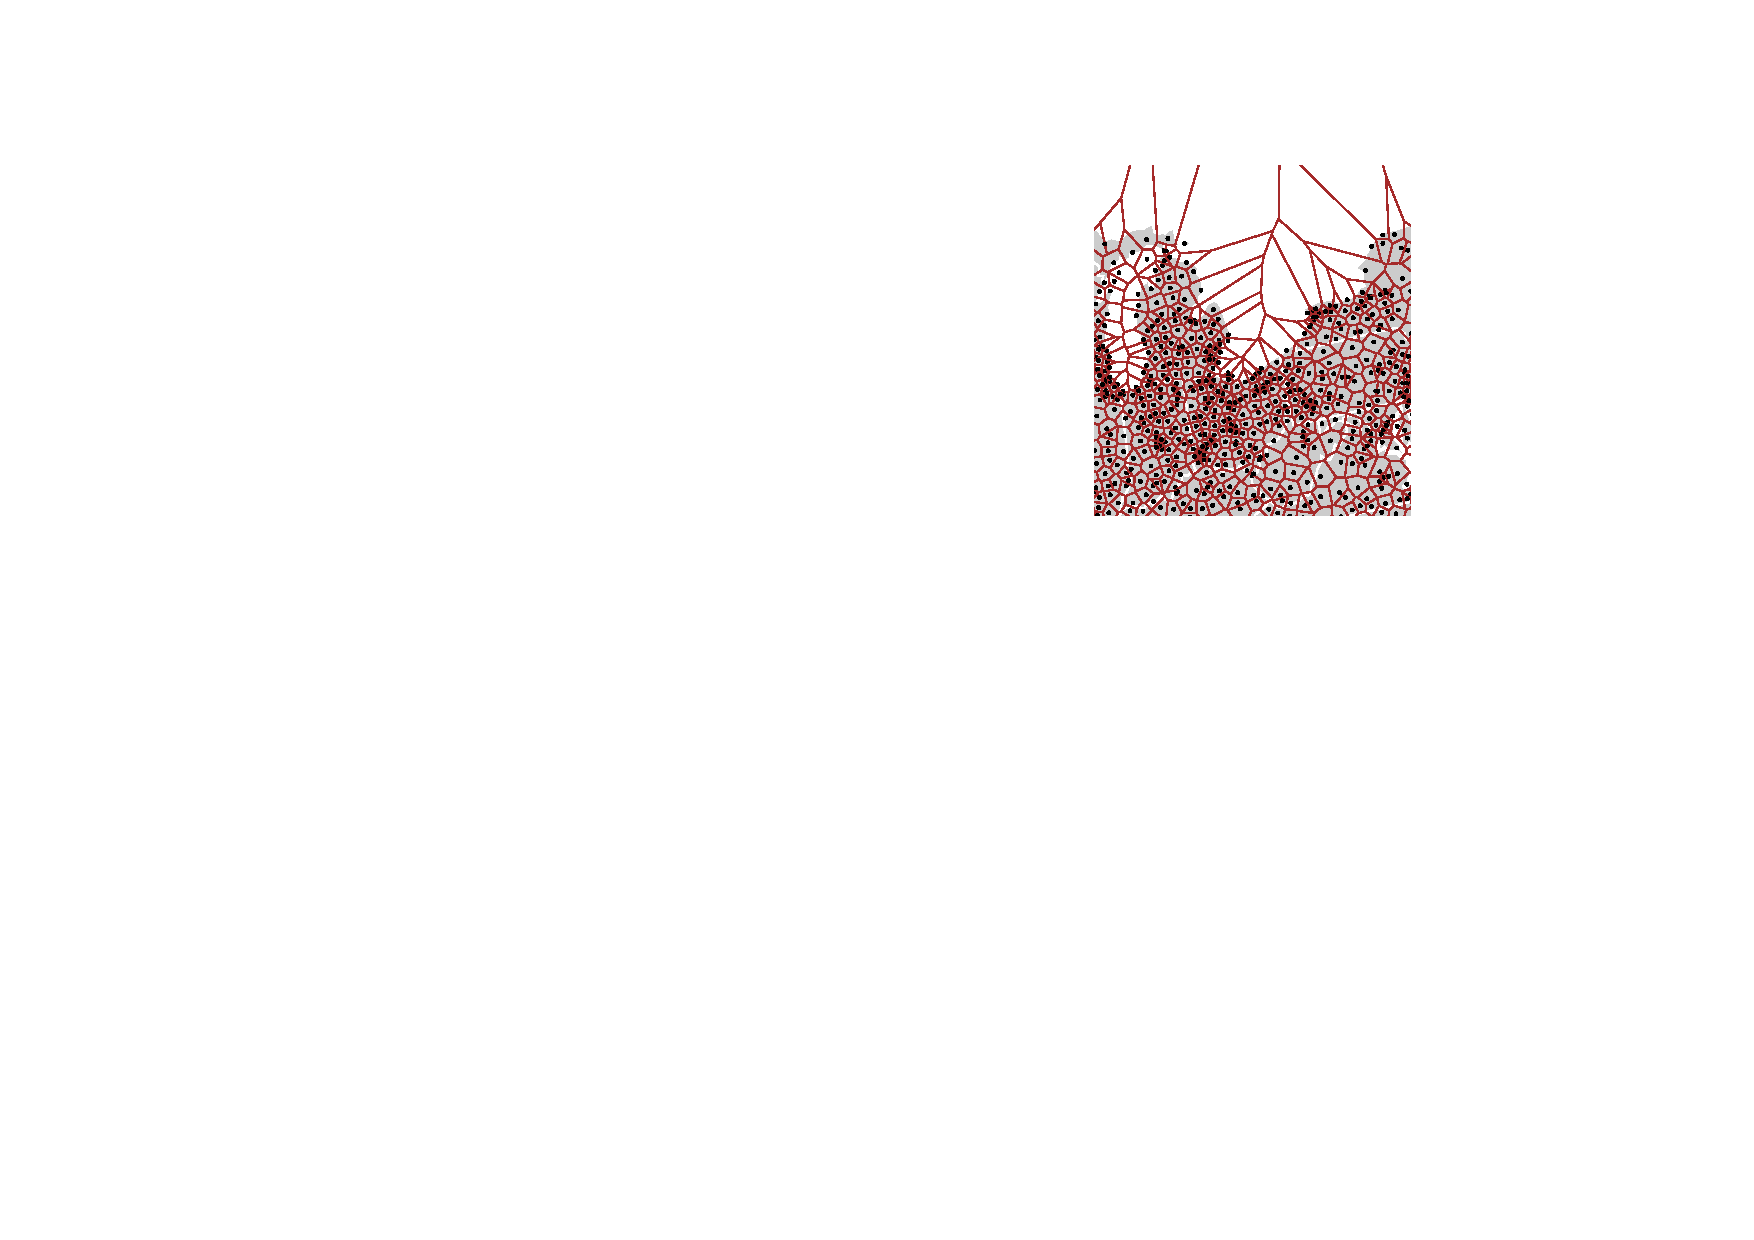
\includegraphics [width=\linewidth]{figures/map_types_voronoi.pdf}
    \captionof {figure}{Voronoi map\protect\footnotemark}
    \label{fig:map-type-voronoi}
}\footnotetext{Voronoi map example \url{http://mbostock.github.io/d3/talk/20111116/airports-all.html}}

\end{itemize}

Self-organizing maps (SOM) can also be used to visualize clusters of data. But instead of displaying data on a geographic map, self-organizing maps create their own virtual space in order to represent information~\cite{noellenburg11geovis}.  


\subsection{Cluster visualization techniques for maps}
\label{chapter:cluster-vis}

The previous chapter has shown different kinds of map visualization techniques appropriate for displaying clustered data. In the end, each visualization will show (clustered) items on a map as objects with attributes like a particular shape or coloring. As clusters contain aggregated information, the task is to find the right way for visualizing the cluster items themselves. From the examples so far, we have seen variations in size, shape and color which expose information on the cluster items being visualized on the map. In the following, multivariate data visualization techniques will be evaluated for visualizing cluster items on a map.

In chapter \ref{vis-data-techniques}, a classification of visualization techniques by data type and interaction technique has been presented. Ke-Bing Zhang~\cite{zhang07thesis} has written about ``Visual Cluster Analysis in Data Mining'' where he list an extensive list of multivariate data visualization techniques. Potentially any such visualization technique can be used, but the frame of the map puts constraints in terms of space on the representation of individual items. Iconic displays are a simple way to visualize data, which also prevents clutter. Dense Pixel displays and geometric visualizations like charts can be used to encode more complex information.

\begin{itemize}

\item \textbf{Icon-based, Glyphs}

Matthew O Ward \cite{ward02glyphs} defines \textit{glyphs} as ``graphical entities that convey one or more data values via attributes such as shape, size, color, and position''. While the work of Otto Neurath on ISOTYPE~\cite{neurath} (1930s) can be seen as fundamental for pictorial statistics, the best-known literature reference to glyphs is ``Chernoff faces''~\cite{chernoff73}. As indicated in (e) of figure \ref{fig:glyphs-ward}, data is encoded into properties of the face icon, such as shape of nose, mouth, eyes. Other fundamental glyph-based techniques include stick figures~\cite{stickfigures}, color icons~\cite{coloricons}, Hyperbox~\cite{hyperbox} and shape coding~\cite{shapecoding}. Figure \ref{fig:glyphs-ward} extends this list by showing examples of glyphs that Ward collected for his taxonomy of glyphs placement strategies~\cite{ward02glyphs}.

\begin{figure}[h]
  \begin{center}
    \hspace*{-1cm}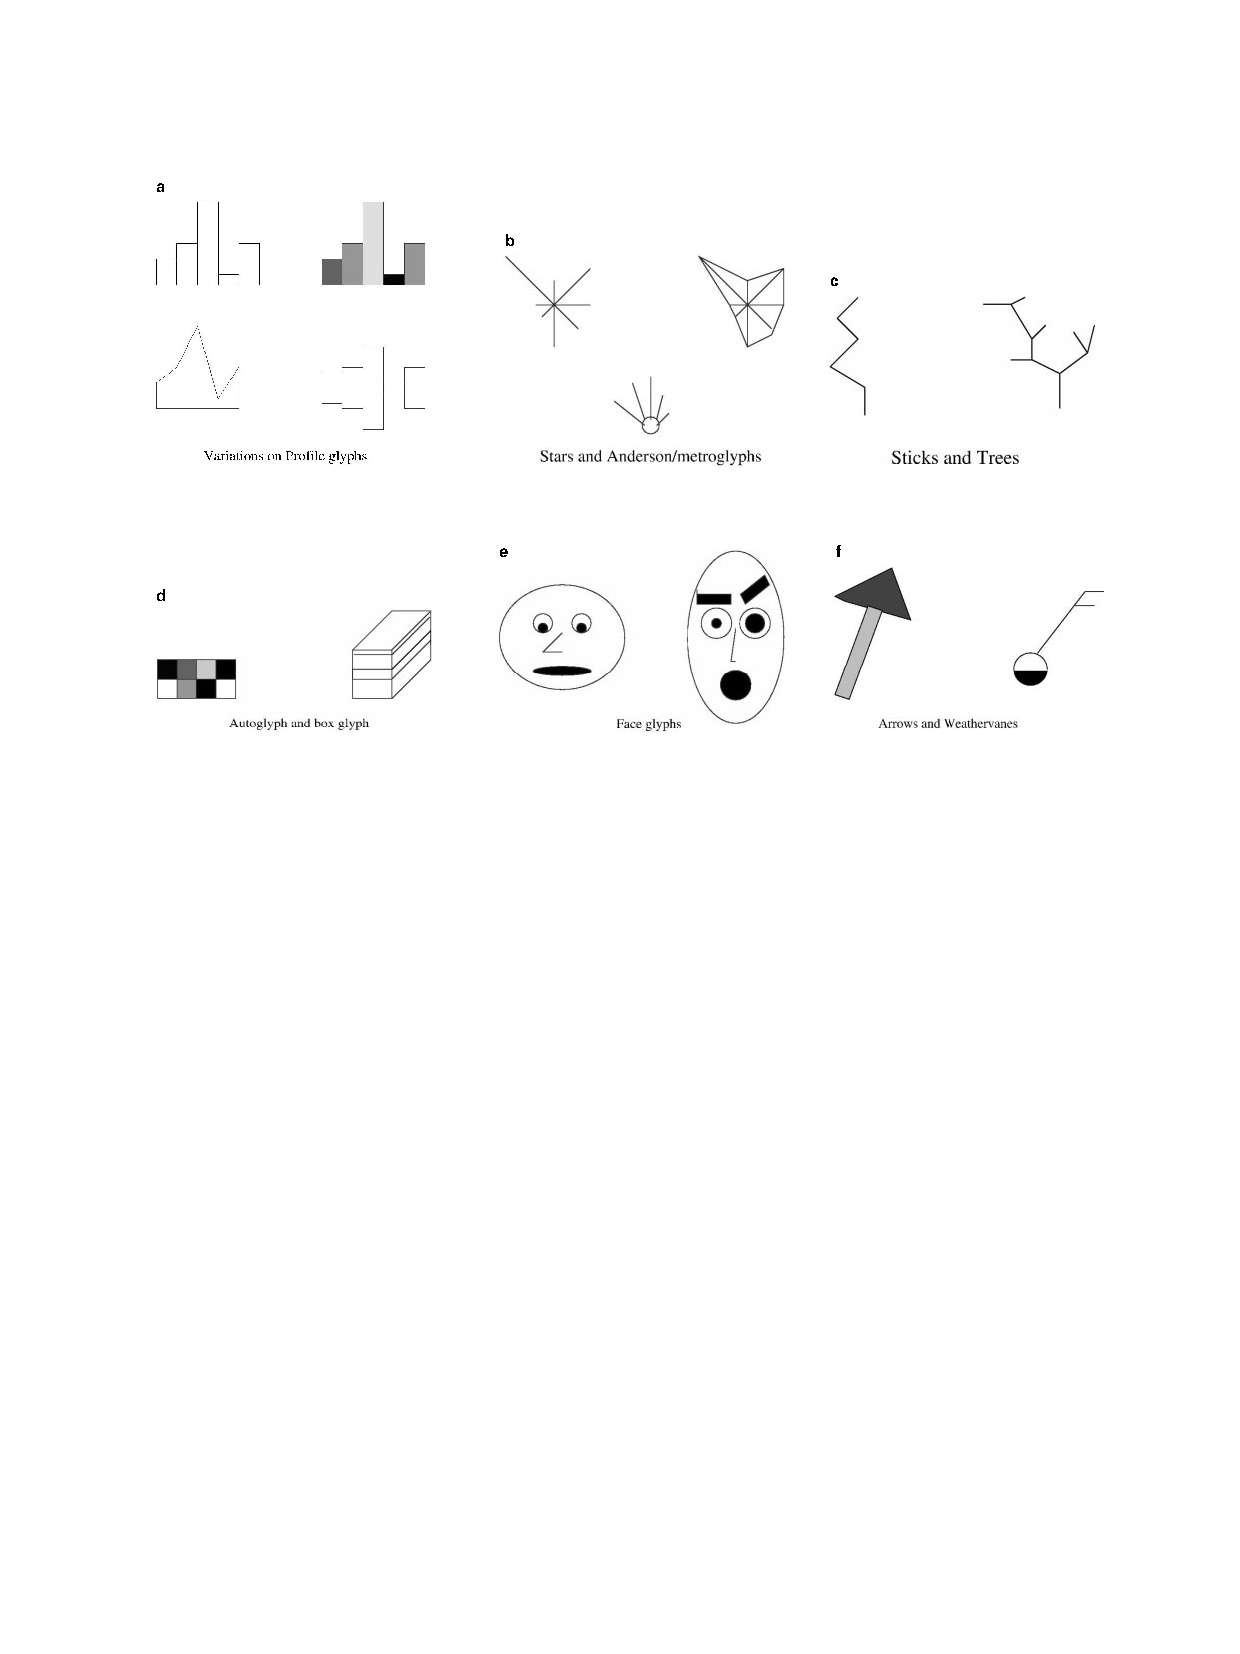
\includegraphics[width=1.2\textwidth]{figures/glyphs.pdf}
    \caption{Examples of glyphs. Top row: (a) variations on profiles; (b) stars/metroglyphs; and (c) stick figures and trees.
Bottom row: (d) autoglyphs and boxes; (e) faces; and (f) arrows and weathervanes.~\cite{ward02glyphs}.}
    \label{fig:glyphs-ward}
  \end{center}
\end{figure}

Some glyph types have been created to identify clusters or similarities by plotting them side-by-side on a 2-dimensional plane, a technique which is referred to as mosaic-based rendering. Stick figures and mosaic metaphors are examples in that field~\cite{stickfigures, nocke05mosaic}. One the other hand, reducing visual clutter as explained in chapter \ref{clutter-reduction} also matters for glyphs, especially when putting them on a map. A trade-off between information-richness vs. simplicity and clarity has to be made. As Zhang writes ``the amount of data increasing, the user hardly makes any sense of most properties of data intuitively, this is because the user cannot focus on the details of each icon when the data scale is very large''~\cite{zhang07thesis}. We can compare this to the map use cube presented in chapter \ref{chapter:foundations-vis}: more complex glyph types seem to be better suited for scientific purposes which can be related to private uses, while simpler glyph types can be used for presenting data to a public audience.

Examples for uses of simple icons and glyph types for clustered data on maps can be found in JavaScript mapping libraries as seen in chapter \ref{chapter:client-side-web-mapping}. These are usually based on a simple icon or geometric shape like a circle or marker and use color coding and size variations as indicators for underlying information. Figure \ref{fig:glyphs-zame} visualizes eight simple glyphs~\cite{ElmqvistDGHF08}. Further examples are scaled data values and scaled dots \cite{web:scaled-data-value}, as well as the proportional symbol map \cite{vislecture}.

\begin{figure}[h]
  \begin{center}
    
\includegraphics[width=0.65\textwidth]{figures/glyphs_zame.pdf}
    \caption{Eight different glyphs for aggregated edges (color shade,
average, min/max histogram, min/max range, min/max tribox, Tukey
box, smooth histogram, step histogram)~\cite{ElmqvistDGHF08}.}
    \label{fig:glyphs-zame}
  \end{center}
\end{figure}


\item \textbf{Pixel-oriented}

Pixel-oriented techniques display the most possible information at a time but mapping each attribute value of data to a single colored pixel. Color mapping approaches such as linear variation of brightness, maximum variation of hue and constant maximum saturation are used to color pixels which are arranged adequately in limited space. By providing an overview of large amounts of data, pixel-oriented display techniques are suitable for a variety of data mining tasks of large databases~\cite{zhang07thesis}.

The first pixel-oriented technique was presented by Keim~\cite{keim94pixel} as part of the VisDB system. Large amounts of multidimensional data could be represented as Spirals and Axes. Figure \ref{fig:pixel-spiral} illustrates how a spiral would be constructed and figure \ref{fig:pixel-axes} shows a rendered result of the axes technique. Further developments include the Recursive Pattern Technique \cite{keim95recpat} and the Circle Segments Technique \cite{Ankerst96circlesegments}. Figure \ref{fig:pixel-circle} visualizes such a circle which represents about 265,000 50-dimensional data items.

While no real-world examples have been identified during the research, using pixel-oriented techniques for visualizing complex clusters on a map seems possible. As the visualization relies on a large amounts of multidimensional data being present within clusters, the clustering algorithm would need to provide such required data. Performance implications also need to be considered, as potentially multiple clusters have to be visualized on a map, sometimes even in real-time.

\hspace*{-2cm}\parbox [h]{0.35\textwidth }{
    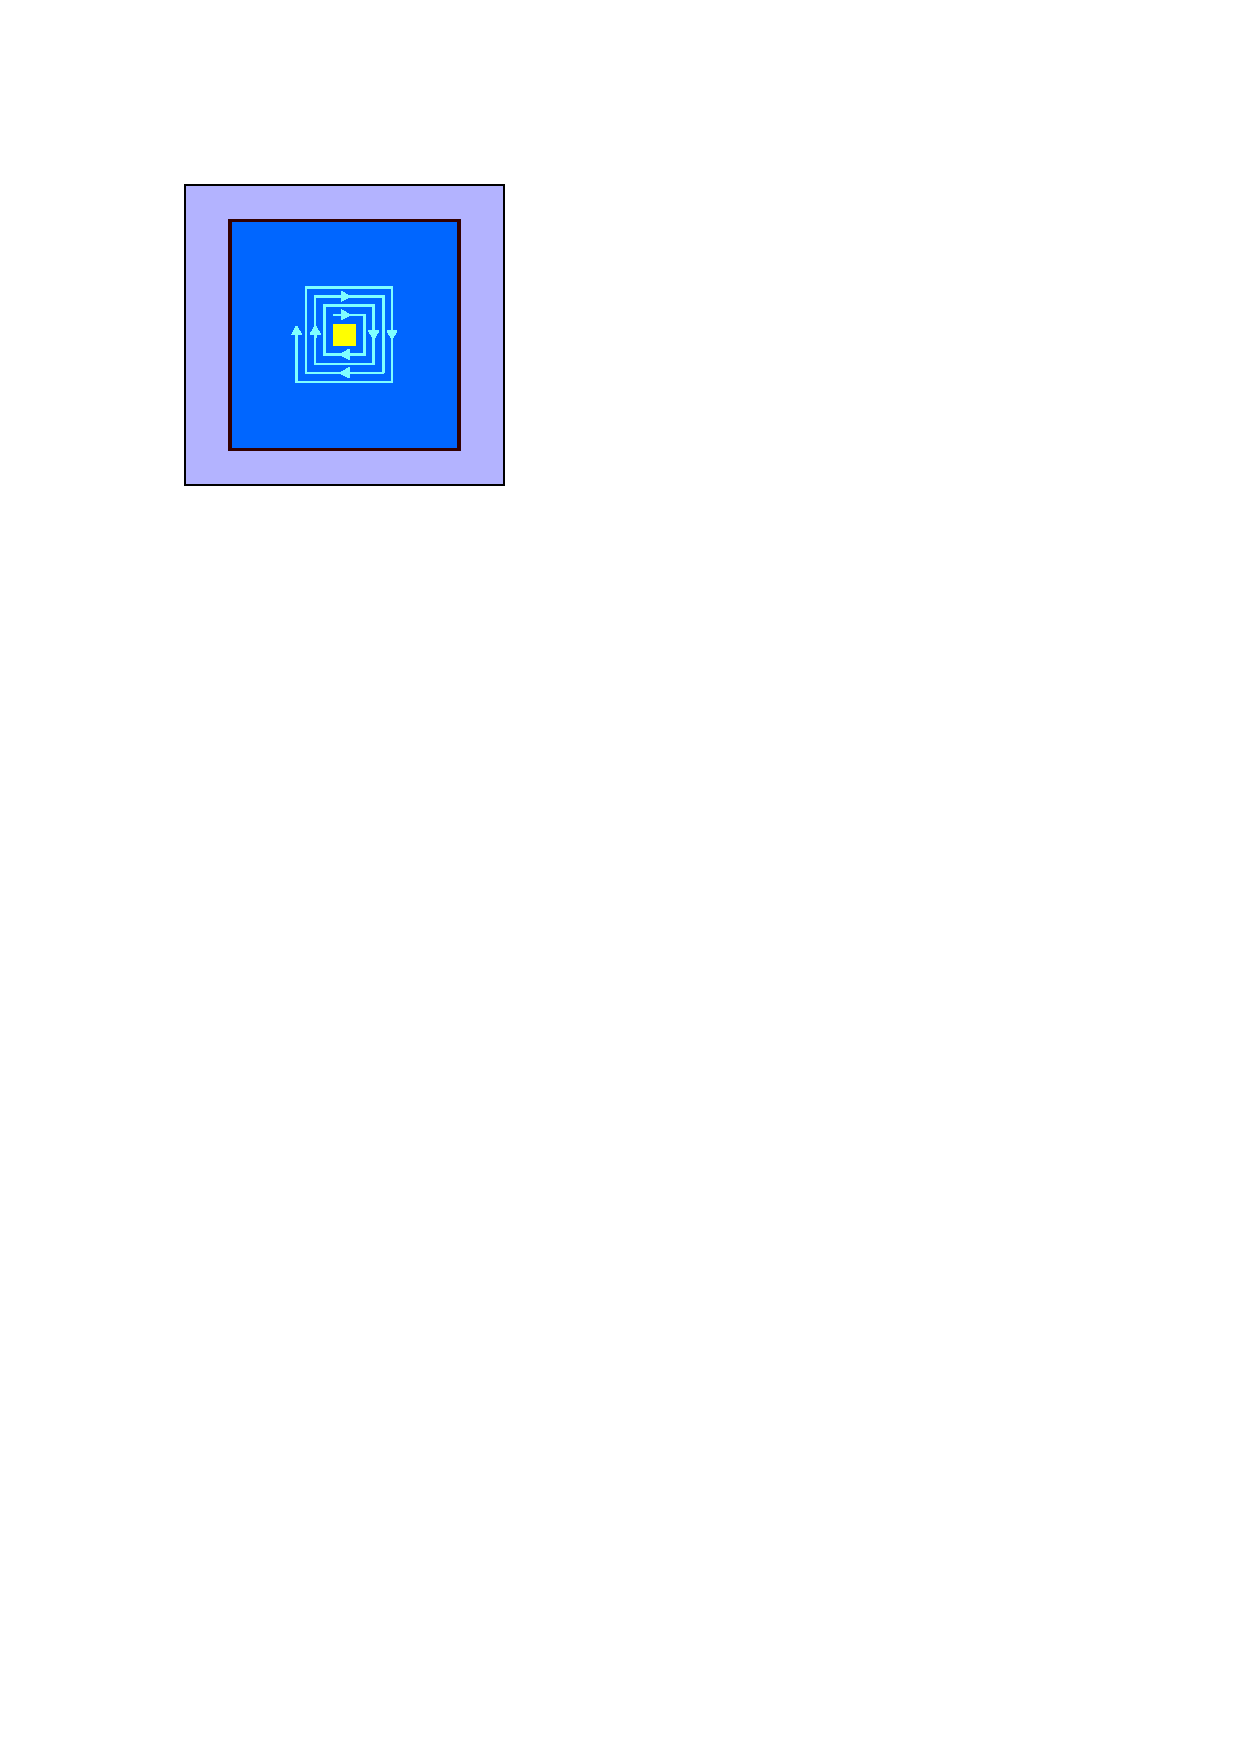
\includegraphics [width=\linewidth]{figures/pixel_keim_spiral.pdf}
    \captionof {figure}{Spiral~\cite{keim94pixel}}
    \label{fig:pixel-spiral}
}
\hfill
\parbox [h]{0.33\textwidth }{
    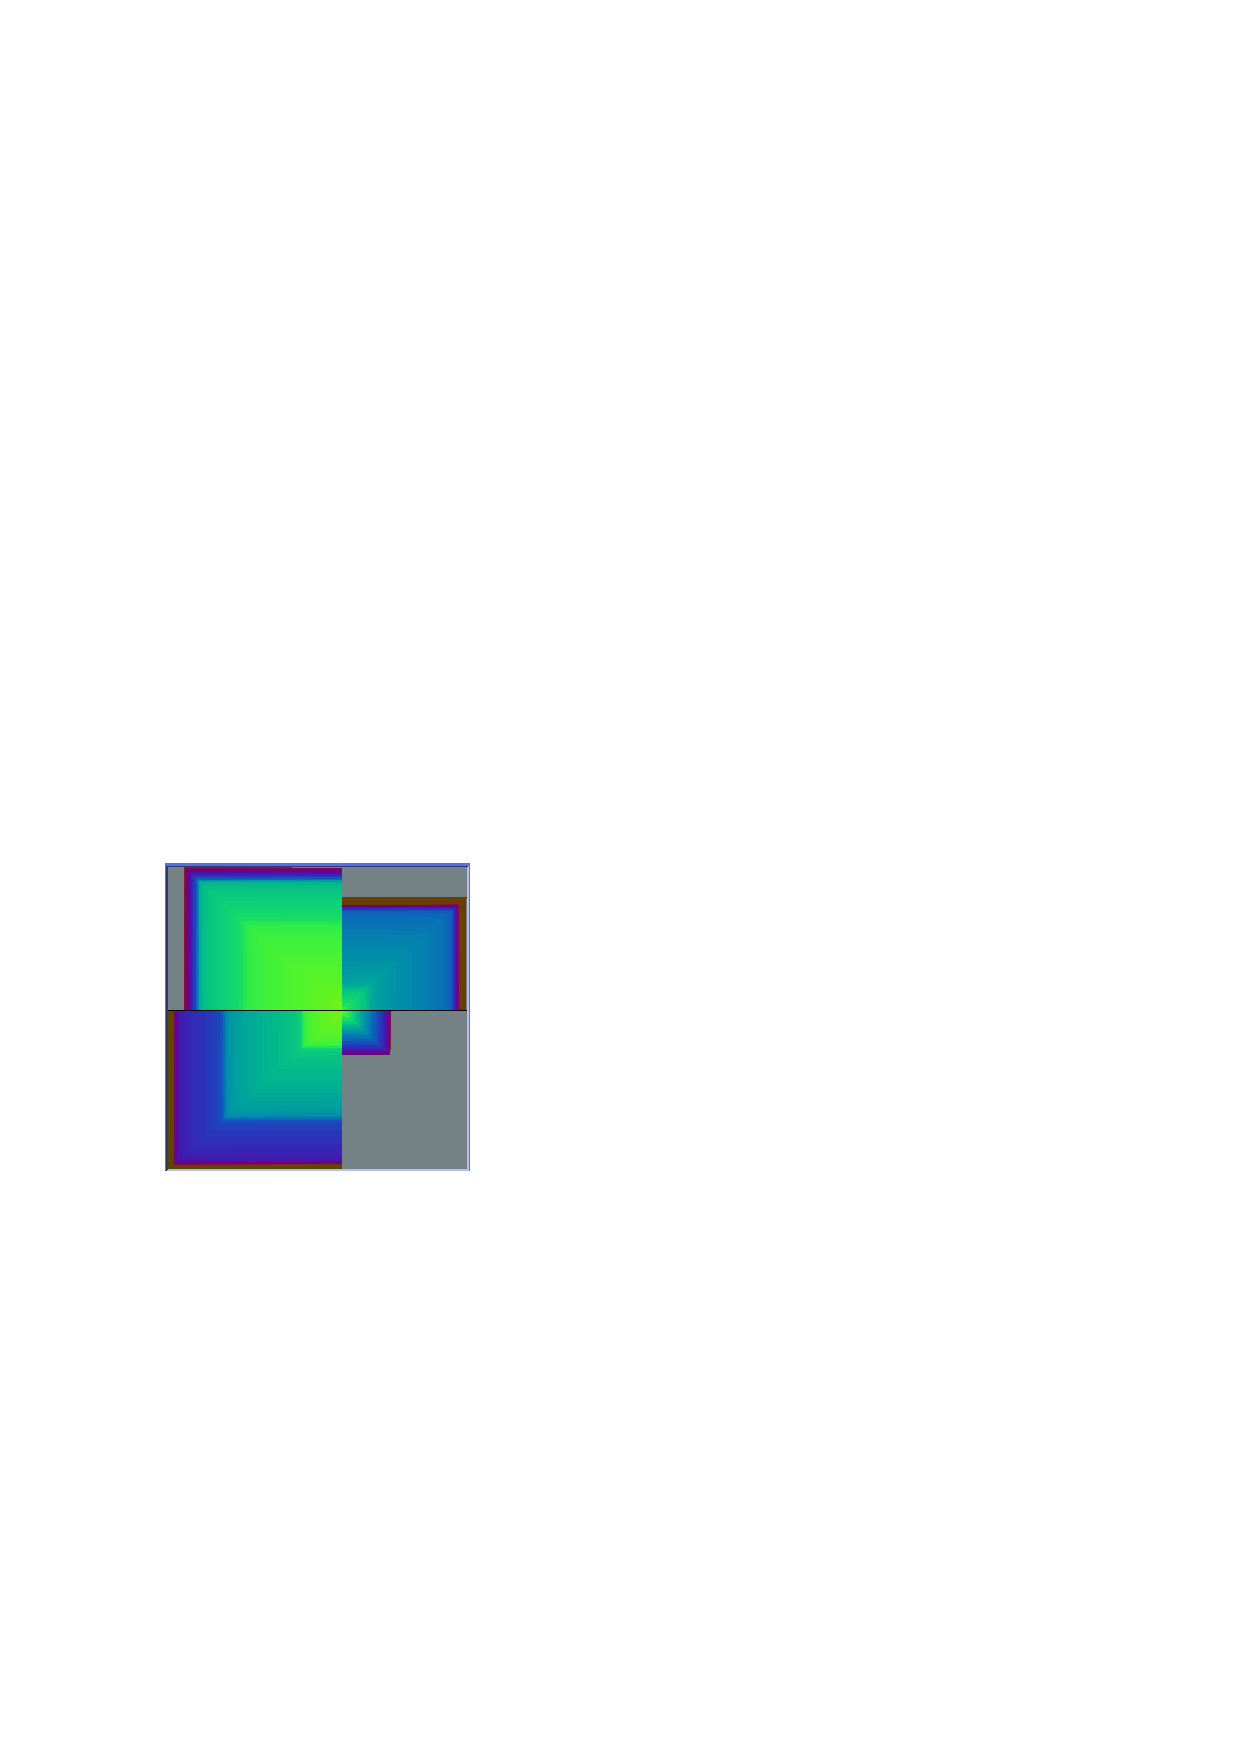
\includegraphics [width=\linewidth]{figures/pixel_keim_axes.pdf}
    \captionof {figure}{Axes \cite{keim94pixel}}
    \label{fig:pixel-axes}
}
\hfill
\parbox [h]{0.35\textwidth }{
    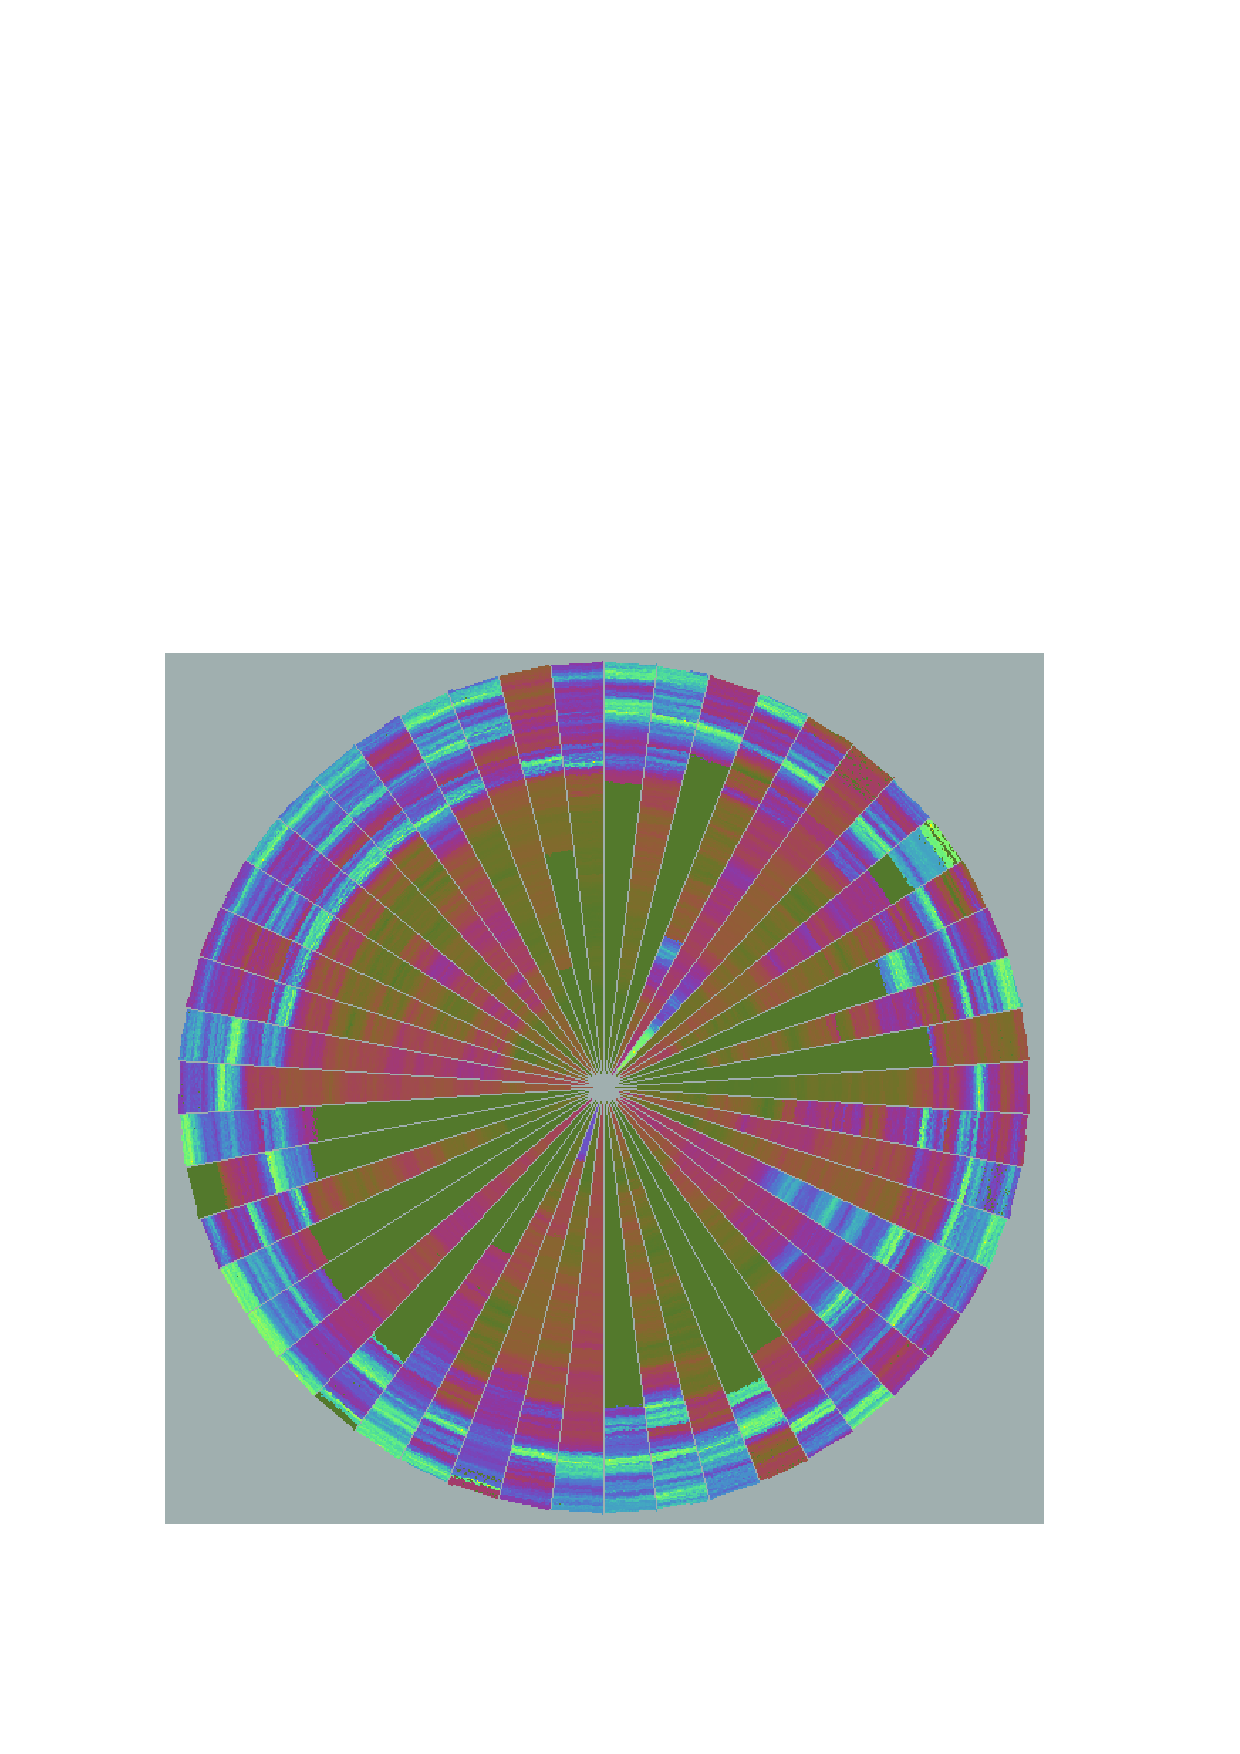
\includegraphics [width=\linewidth]{figures/pixel_keim_circle.pdf}
    \captionof {figure}{Circle \cite{Ankerst96circlesegments}}
    \label{fig:pixel-circle}
}


\item \textbf{Geometric techniques \& Diagrams}

Geometric techniques produce useful and insightful visualization by using geometric transformations and projects of the data.  Diagrams are algorithmically drawn graphics that visualize data. This section lists a selection of geometric techniques for multivariate data presented by Ke-Bing Zhang~\cite{zhang07thesis}, diagram types described by Dieter Ladenhauf~\cite{ladenhauf12dia} and related examples found in additional literature and on the web as stated in the individual references.

\begin{itemize}

\item \textit{Line charts} visualize data as lines by connecting data points of the corresponding values. They are used to display trends over time. Figure \ref{fig:dia-map-sparklines} illustrates surface temperature anomalies from NASA's GISS as Spark line map~\cite{web:sparkmaps}. The Sparkline is a reduced line chart without axes and coordinates. It presents the general shape of variation in a simple and highly condensed way~\cite{wiki:sparkline}.

\item \textit{Bar charts} express data values by vertical or horizontal bars, in which the length of a bar indicates the data value. Figure \ref{fig:dia-map-barchart} shows an example from UgandaWatch which shows economic indicators per region for the country Uganda. In this example, the Drupal mapping stack explained in chapter \ref{chapter:drupal-mapping} is extended by bar chart technologies\footnote{\url{http://groups.drupal.org/node/174904\#comment-585264}}.

\parbox [h]{0.4\textwidth }{
    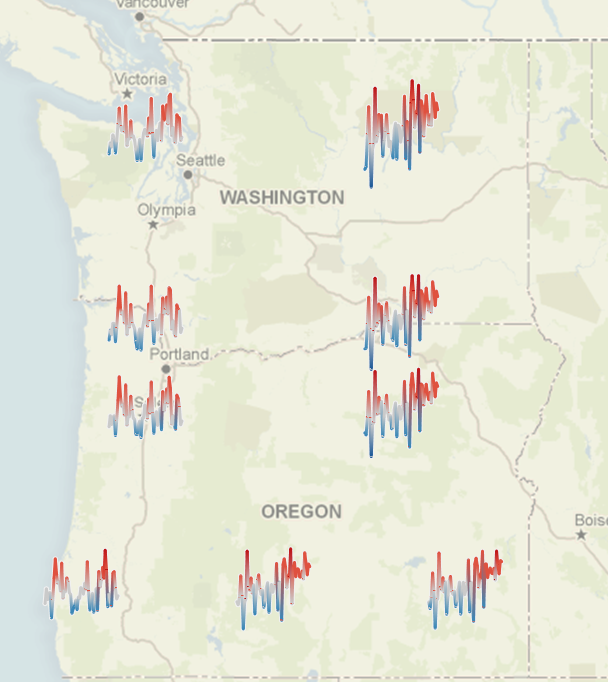
\includegraphics [width=\linewidth]{figures/dia_map_sparklines.png}
    \captionof {figure}{Spark line map\protect\footnotemark}
    \label{fig:dia-map-sparklines}
}\footnotetext{Spark line map example: \url{http://www.tableausoftware.com/about/blog/2008/08/sparklines-maps}}
\hfill
\hspace{0.5cm}
\parbox [h]{0.4\textwidth }{
    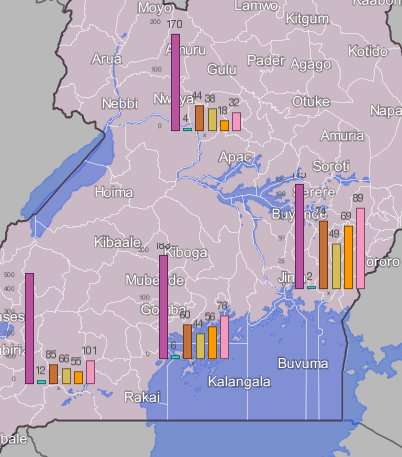
\includegraphics [width=\linewidth]{figures/dia_map_barchart.png}
    \captionof {figure}{Bar chart map\protect\footnotemark}
    \label{fig:dia-map-barchart}
}\footnotetext{UgandaWatch bar chart example: \url{http://www.ugandawatch.org/}}


\item \textit{Pie charts} use a circle divided into sectors for expressing the proportional significance of data values. Variants of pie charts include doughnut charts, three-dimensional pie charts and multi-level pie charts. Also, the polar area diagram introduced in figure \ref{fig:map-type-standard-wind} is a special kind of pie chart which is a further development of the Bat's wing diagram by Florence Nightingale~\cite{night98bart}.

Figure \ref{fig:dia-map-piechart} depicts a pie chart map example from Kartograph. It shows unemployment rates in Spain, providing an effective way to display ratios as opposed to a chloropeth map, where the user usually needs to consult a legend to understand the actual data values.

\item \textit{Container shapes} such as bounding boxes and hulls are an alternative to iconic displays as they can show the area covered by clusters~\cite{Delort10vis}. As seen in figure \ref{fig:leaflet}, the Leaflet.markercluster library visualized the convex hull of a cluster to indicate the covered area on mouse-hover. Marco Cristani et al~\cite{Cristani08geoimagemaps} used a hull-based technique to visualize clusters from geo-located image databases on a map. As illustrated in figure \ref{fig:dia-map-hull}, each cluster is represented by a hull that marks the boundaries of the area and also shows a representative image of the cluster.


\parbox [h]{0.4\textwidth }{
    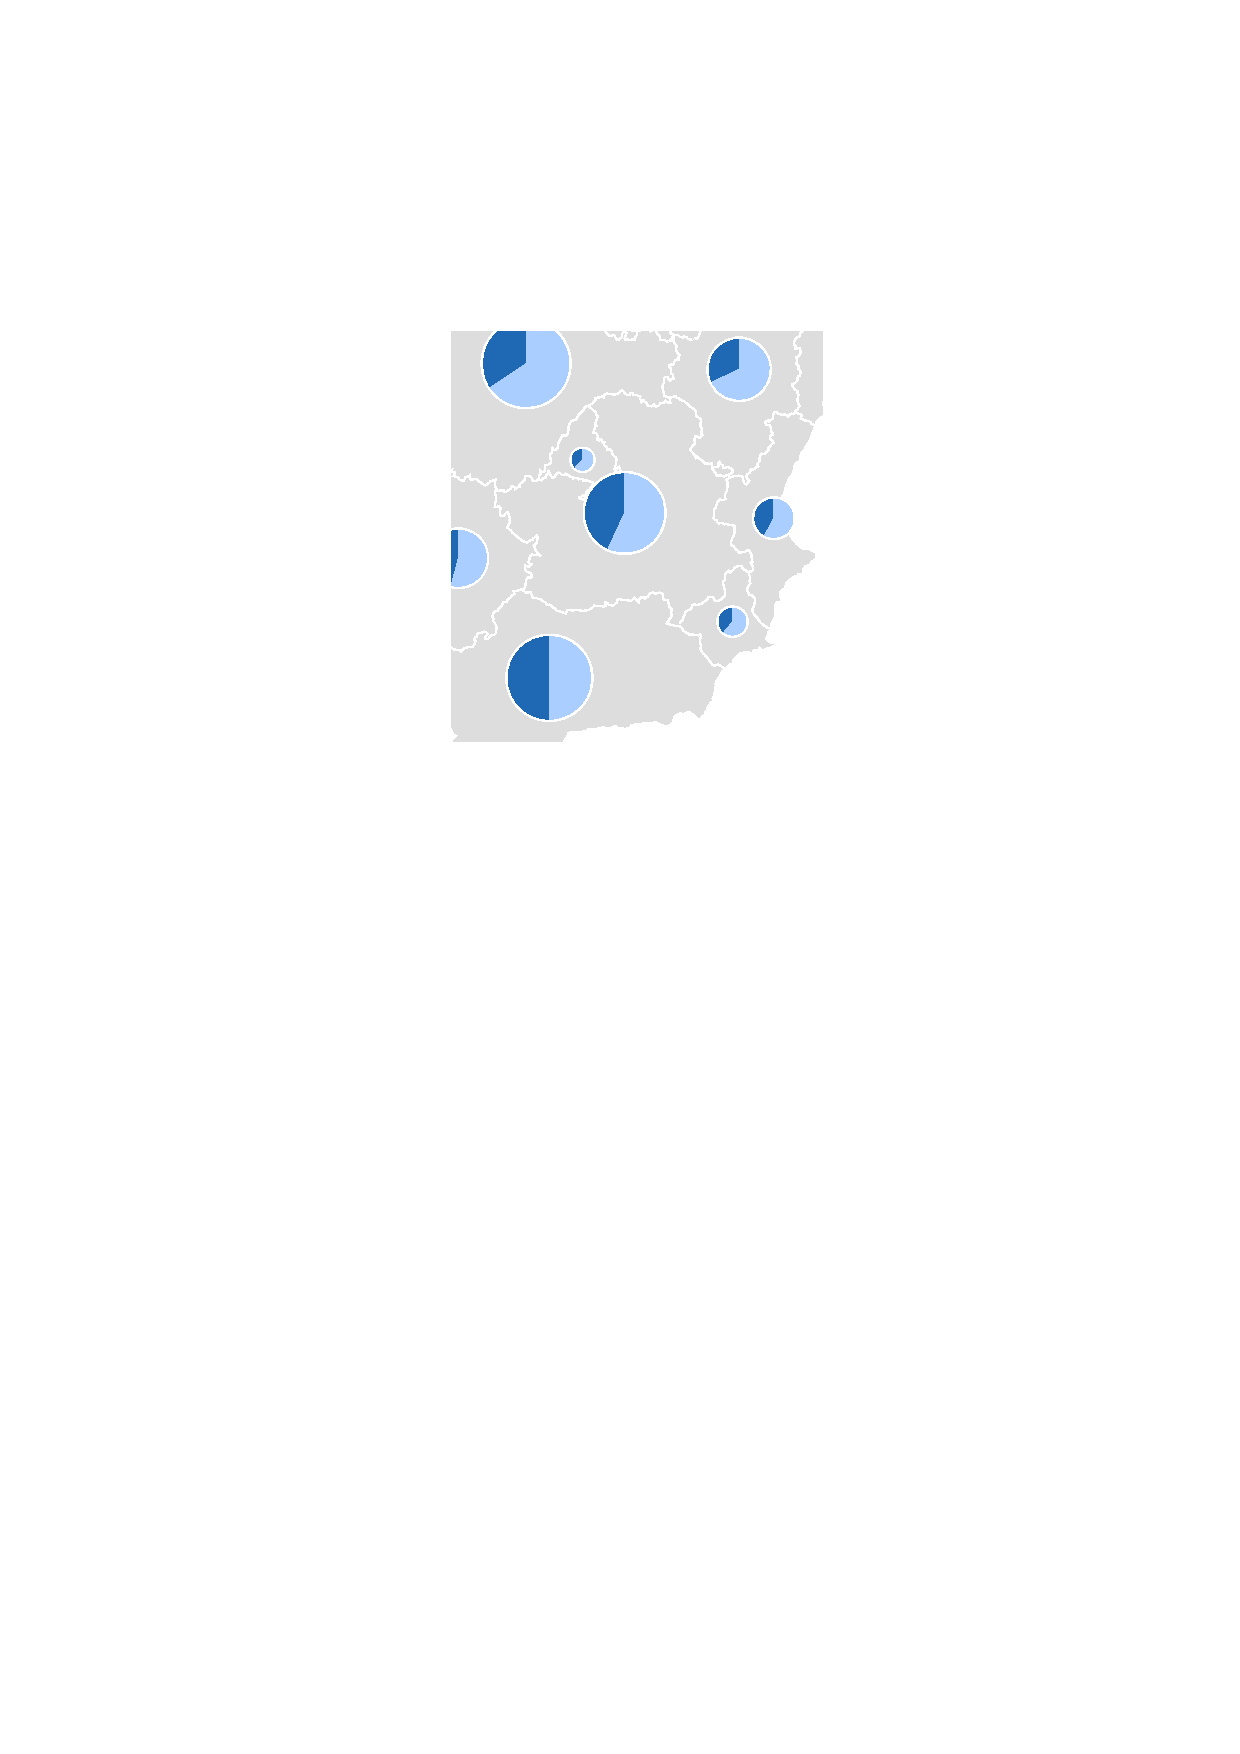
\includegraphics [width=\linewidth]{figures/dia_map_piechart.pdf}
    \captionof {figure}{Pie chart map\protect\footnotemark}
    \label{fig:dia-map-piechart}
}\footnotetext{Pie chart map example from Kartograph: \url{http://kartograph.org/showcase/charts/}}
\hfill
\hspace{0.5cm}
\parbox [h]{0.4\textwidth }{
    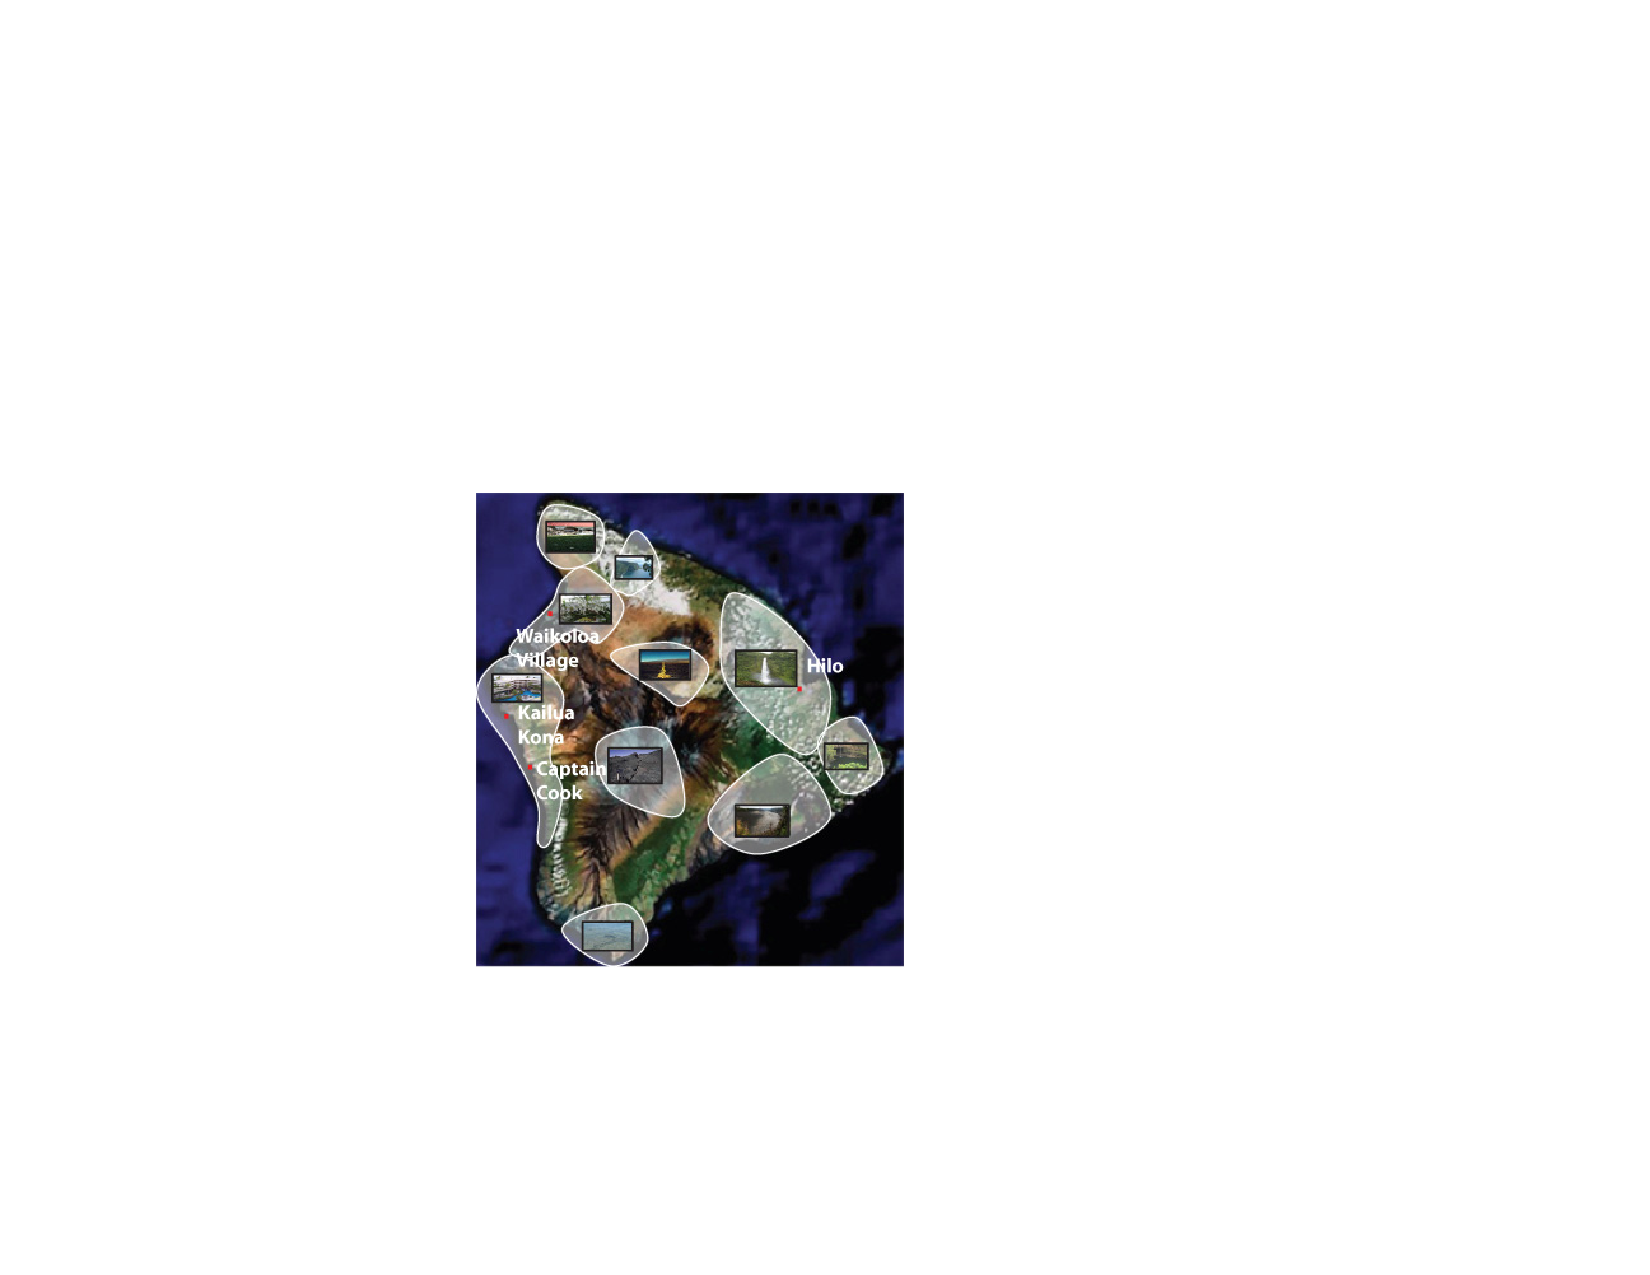
\includegraphics [width=\linewidth]{figures/dia_map_hull.pdf}
    \captionof {figure}{Convex hull map\protect\footnotemark}
    \label{fig:dia-map-hull}
}\footnotetext{Convex hull map example from \cite{Cristani08geoimagemaps}}



\item Further chart types with possible use for visualizing clusters on a map include Area charts and Star plots~\cite{ladenhauf12dia} or more complex ones like Parallel coordinates, Scatterplots, Treemaps~\cite{zhang07thesis} or the Contingency Wheel++~\cite{VAST2012}. Bristle maps are an interesting approach for visualizing spatiotemporal data on a map. Basically, histograms of the data are rendered onto linear map elements. If the data permits a mapping from aggregates to spatial line data, such a visualization technique could be of interest~\cite{bristle}.

\end{itemize}

\end{itemize}

This concludes the stated, investigative enumeration of cluster visualization techniques for maps. It is by no means a complete, but rather an exemplary listing that may provide a starting point when researching visual means to present clustered data on a map.

An interesting publication by Andrienko et al~\cite{andrienko2012sca} presents a complex system for place-oriented analysis of movement data. This goes beyond the use case of simply visualizing clustered data on a slippy map, but it is a good show case for how effective the presentation of spatio-temporal data using a combination of techniques can be. Time graphs, mosaic dioramas, space-time cubes and table lens displays are used to create a powerful tool for inspecting movement data on maps.

\subsection{Evaluation of visualization techniques for clusters on a map}

This chapter summarizes the main visualization examples of the previous chapters. An evaluation of techniques for visualizing clusters on maps is presented by proposing a set of key characteristics that are considered to be significant for the visualization.

Evaluating information visualization techniques is a well-known problem. Undertaking an evaluation that is capable of ``proving'' the effectiveness is impossible in many situations as it would require too many tasks, data sets, implementations and users. Ellis and Dix state exploratory analysis as the most effective approach for evaluating visualization techniques~\cite{ellis06eval, Delort10vis}. In this sense, the following evaluation should primarily be treated as exploratory and as a help for understanding how cluster visualization on maps works, rather than a final, summative conclusion of which technique is superior than another. 

In chapter \ref{chapter:foundations-vis}, three taxonomies have been introduced: \textit{visual variables}, a \textit{classification of visual data exploration techniques} and a \textit{clutter reduction taxonomy}. An attempt to classify the different visualization techniques for representing clusters on maps according to classes introduces by these taxonomies didn't feel valid because the resulting data would not have much value. Instead, the following, custom criteria have been defined: \textit{category}, \textit{shows number of items within cluster} (\textit{by shape size}, \textit{by color or other}), \textit{shows cluster area}, \textit{shows extra cluster info} \textit{(extra cluster info complexity}). Some criteria contain sub-criteria which are stated within parentheses.


A classification based on all visual variables would have become very complex. As the given visualization examples describe concepts, there are many possible variations that would increase the data set even more. It is still helpful to rely on the aesthetic attributes for a better understanding of how each visualization is constructed. Especially the shape, size and color attributes are considered to have a strong effect on visualizing clusters on maps and are therefore included within the evaluation. An explanation of each criterion follows:

\begin{itemize}

\item \textbf{category}: Determines the type of visualization technique being evaluated. Possible values are \textit{type of map} (see chapter \ref{chapter:map-vis}), a visualization \textit{example}, as well as abbreviations for cluster visualization techniques (see chapter \ref{chapter:cluster-vis}): \textit{glyph}: Icon-based, Glyphs, \textit{pixel}: Pixel-oriented techniques and \textit{geom}: Geometric techniques \& Diagrams.

\item \textbf{shape}: Defines the type of shape being used for the visualization of clusters on the map. For example \textit{circle} or \textit{area}. Refer to the visual variable shape in chapter \ref{chapter:vis-variables}. 

\item \textbf{shows \# of items within cluster}: If the visualization provides an indicator of the amount of items per clusters. This relates to the `can see overlap density' criterion of the clutter reduction taxonomy, see \ref{clutter-reduction}. Two sub-criteria are used to differentiate between visual means of encoding the number of items within clusters: 

\begin{itemize}

\item \textbf{by shape size}: classifies visualization techniques that use the shape size for indicating the number of items within clusters.

\item \textbf{by color or other}: classifies visualization techniques that use color or other visual indicators to describe the number of items within a cluster.

\end{itemize}

\item \textbf{shows cluster area}: Determines, if the visualization indicates the spatial area that is covered by the cluster or the items within a cluster.

\item \textbf{shows extra cluster info}: Besides the two characteristics of number of items within a cluster and the cluster area, the technique might provide means of visualization additional information of clusters such as aggregates. 

\begin{itemize}

\item \textbf{extra cluster info complexity}: This sub-criterion expands of an intuitive notion of complexity that can be visualized as extra cluster info by the technique. \textit{low} indicates a maximum of three dimensions. \textit{medium} is used to describe up to 12 dimensions of additional data and \textit{high} classifies cluster visualization techniques that go beyond this number of dimensions.

\end{itemize}

\end{itemize}

\begin{figure}[h]
  \begin{center}
    \hspace*{-1.5cm}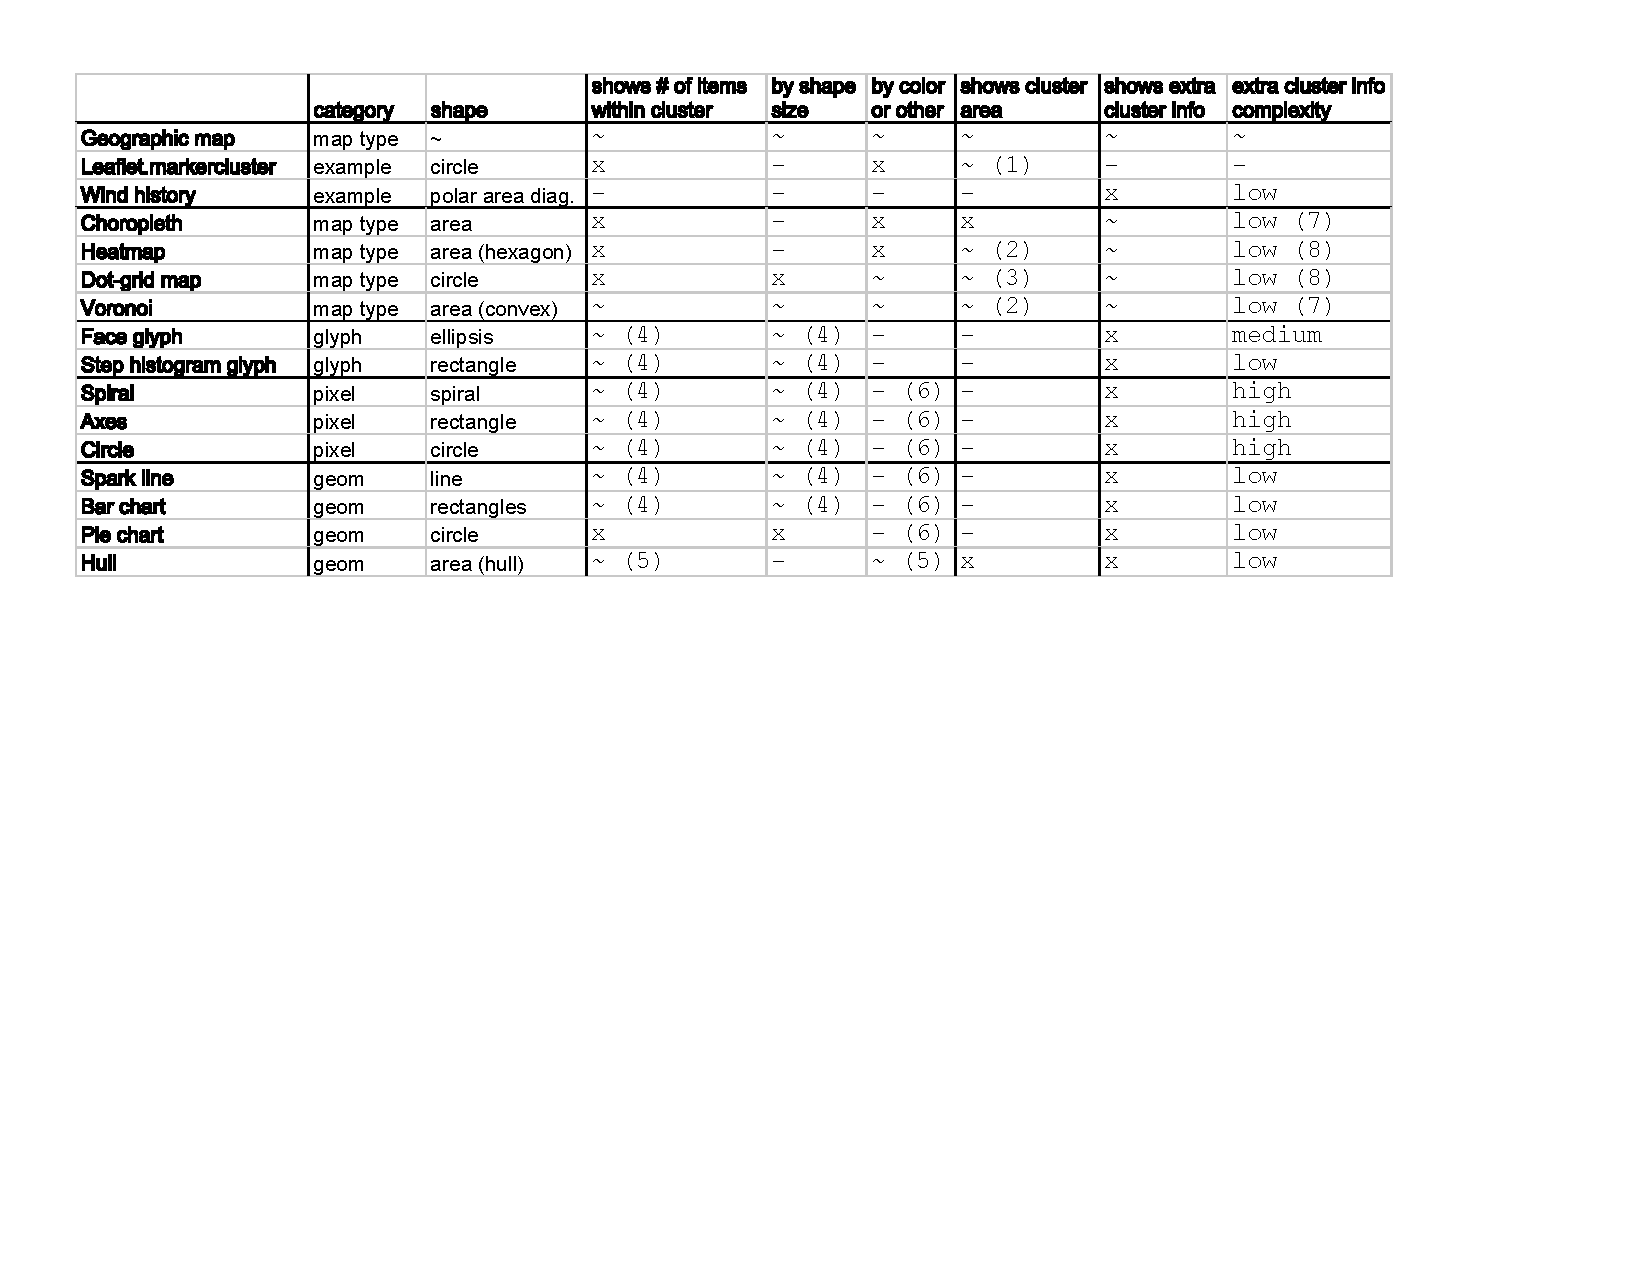
\includegraphics[width=1.2\textwidth]{figures/vis_evaluation.pdf}
    \caption{Evaluation of visualization techniques for clusters on a map. Legend:~`x':~yes,~`\textasciitilde': possibly, `-': no. Numbers in parentheses reference additional notes within the accompanying text.}
    \label{fig:vis-eval}
  \end{center}
\end{figure}

The results of the evaluation of visualization techniques for clusters on a map based on the stated criteria are illustrated in figure \ref{fig:vis-eval}. Note that the classifications for each technique being evaluated primarily represent the according examples shown in the previous chapters. Where it seemed obvious, the optional possibility of fulfilling a criterion has been marked as such. As an extreme example, the geographic map as its general concept has been marked with the optional possibility of fulfilling each criterion. It is up the the actual implementation to satisfy them individually. While the Leaflet.markercluster example provides a visual indicator for the number of items within clusters, the wind history example doesn't.

Some classifications contain a number referring to additional notes as presented in the following: (1) The Leaflet.markercluster example shows cluster on demand, based on user interaction. By mouse-hovering over an item, it will display the convex hull of the items being clustered, see figure \ref{fig:leaflet}. (2) In the case of the binned heat map example and the Voronoi map, cluster areas are approximated by the tessellation which is part of the clustering algorithm, see figure \ref{fig:map-type-binning} and \ref{fig:map-type-voronoi}. (3) The dot-grid map doesn't provide a mean of showing cluster areas by themselves, but the density of items still supports the notion of recognizing cluster areas, see figure{fig:map-type-dotgrid}. (4) For various visualization techniques, the amount of items within a cluster could be visualized by simply scaling the visual entity. (5) The hull example uses an area shape defined by the data, similarly to the choropleth map. Without a distortion technique, the shape therefore can't be used to indicate the number of items within a cluster. Still, a non-shape visual aspect like color could be used as an indicator. (6) In the case of pixel-oriented techniques and the provided chart examples, the color attribute will likely be used for showing extra cluster info instead of indicating the number of items within a cluster. Modifying the shape size can be used as an alternative in this cases. (7) The choroleth and voronoi map examples would rely on representing extra information within the defined area and therefore rely on the.variation of visual variables related to color and texture. (8) The same restrictions as in the previous note apply, but for even smaller areas.

Driving forces in visual mapping, map visualization types and cluster visualization techniques for maps have been introduces and summarized within the given evaluation. This concludes the chapter on state of the art. 




%
% objectives
%

\chapter{Objectives}
\label{chapter:objectives}


\section{Performant real-time clustering}
\label{chapter:objective-performance}

The main purpose of this thesis is to design and implement an algorithm that allows to create performant, scalable maps with Drupal by using server-side clustering in real-time. The algorithm needs to dynamically cluster geospatial data on the server-side, before it is rendered by Drupal and gets transferred to the client. As a result, the client-side mapping visualization component receives a limited amount of clustered data which can be processed and visualized efficiently enough to produce a smooth end-user experience.

The expected performance benefits of using a server-side geo clustering component to be designed and implemented for Drupal are:

\begin{enumerate}

\item Better server performance by only processing (pre-)clustered items
\item Better network performance by only transferring clustered items 
\item Better client performance by only processing and visualizing clustered items 

\end{enumerate}

The goal is to build upon existing cluster theory, the current state of the art and the existing Drupal mapping capabilities. The following requirements apply for a successful clustering implementation:

\begin{itemize}

\item Cluster in real-time to support dynamic queries
\item Cluster up to 1,000,000 items within less than one second.

\end{itemize}



\section{Visualization \& Usability}
\label{chapter:objective-usability}

Clustering data on maps not only affects performance, it also changes the way, the user will see and interact with the clustered data. Ideally, the clustering process should support the user in the task of exploring a large data set on the map by compacting the amount of information that is visualized. The way, how the clustered data is visualized on the map needs to communicate essential information about the clustered data like the size of a cluster. In addition, the user needs means of interacting with the clustered data being presented. The user should be able to reveal the details of clustered data for example by zooming in. 



\section{Integration and extensibility}
\label{chapter:objective-integration}

The server-side clustering implementation should be designed for integration and extensibility. Integration should be provided or at least be possible with key components of the existing ecosystem for creating interactive-maps with Drupal as explained in \ref{chapter:drupal-mapping}. There is also a need for means of extensibility within the clustering solution to facilitate further improvements of the clustering implementation.

The intended benefits of an integrated and extensible approach for the server-side clustering solution are:

\begin{itemize}

\item Integrate the clustering with JavaScript mapping libraries\\ as Leaflet or OpenLayers.

\item Integrate the clustering with Drupal and Apache Solr search backends.

\item Allow to extend the clustering for adding alternative algorithms. 

\end{itemize}


\section{Open source}
\label{chapter:open-source}

One of the main reasons for the wide adoption of Drupal as a content management system and framework is its licensing under the terms of the GNU General Purpose License (GPL). Being free and open source software gives any user the freedom to run, copy, distribute, study, change and improve the software. The intended server-side clustering solution would build upon the Drupal system and a number of extension modules essential to the creation of interactive-mapping solutions. Not only as a logical consequence, but also as a primary factor of motivation, the results of this thesis and in particular the clustering implementation should be released under the free and open source GPL license.

An open process of planning, designing and developing a server-side clustering solution is intended to bring a number of benefits in contrary to a proprietary, closed source approach:

\begin{itemize}

\item The ability to discuss ideas and incorporate feedback from the community during the planning phase.

\item The possibility for other community members to review prototypes and look at the source code.

\item The potential for test results submitted by other community members, testing the solution. 

\end{itemize}


\section{Use cases}
\label{chapter:objective-use-cases}

The practical use case for server-side geo clustering should add spatial search capabilities to the \textit{Recruiter} job board solution.

\begin{quote}
Recruiter is a Drupal distribution for building Drupal based e-recruitment platforms. Users can register either as recruiter and post job classifieds or they can register as applicants and fill out their resume. A faceted search helps users to find jobs and possible job candidates.\footnote{\url{http://drupal.org/project/recruiter}}
\end{quote}

Adding server-side geo clustering capabilities would allow to visualize several thousands of available jobs on an interactive map for large-scale e-recruitment websites. The server-side clustering solution should be designed for the possibility to be added to geospatial searches realized in combination with the Recruiter distribution. This influences the integration and extensibility requirements, stated in the previous chapter.


















%
% realization
%

\chapter{Realization}

TODO

Realization
	Analysis
	
	Algorithm

	Architecture

	Implementation
	
	Project phases


%
% use cases
%

\chapter{Use cases}
\label{chapter:use-cases}

\section{Demo Use Cases}
\label{chapter:use-case-demo}

A set of demonstration use cases has been created in order to test and evaluate the Geocluster implementation described in chapter \ref{chapter:architecture-implementation}. The set consists of one non-clustering map and 3 maps based on the different clustering algorithms. The demo use cases were configured using various Drupal modules and exported into code using the Features module\footnote{\url{http://drupal.org/project/features}}.

\begin{itemize}

\item \textbf{Geocluster Demo} show cases maps based on the two clustering algorithms provided by Geocluster module: PHP-based clustering and MySQL-based clustering and an additional map that doesn't use clustering at all. The article content type of a standard Drupal installation is extended by a Geofield-based place field for storing locations. For each map, a separate View is configured to provide a GeoJSON feed. A Leaflet map is then added on top of the feed by using the Leaflet GeoJSON module. Figure \ref{fig:geocluster-demo-site} illustrates a screenshot of a Geocluster Demo installation.

\item \textbf{Geocluster Demo Solr} adds a show case of the Solr-based clustering algorithm. It provides a setup based on Views GeoJSON and Leaflet GeoJSON similar to the Geocluster Demo feature. In addition, a Search API Server and Index configuration is added for indexing and querying the data using Apache Solr.  

\item \textbf{Geocluster Demo Content} is a sub-module that automatically imports a set of demo content for testing the Geocluster Demo and Geocluster Demo Solr features.

\end{itemize}

\begin{figure}[h]
  \begin{center}
    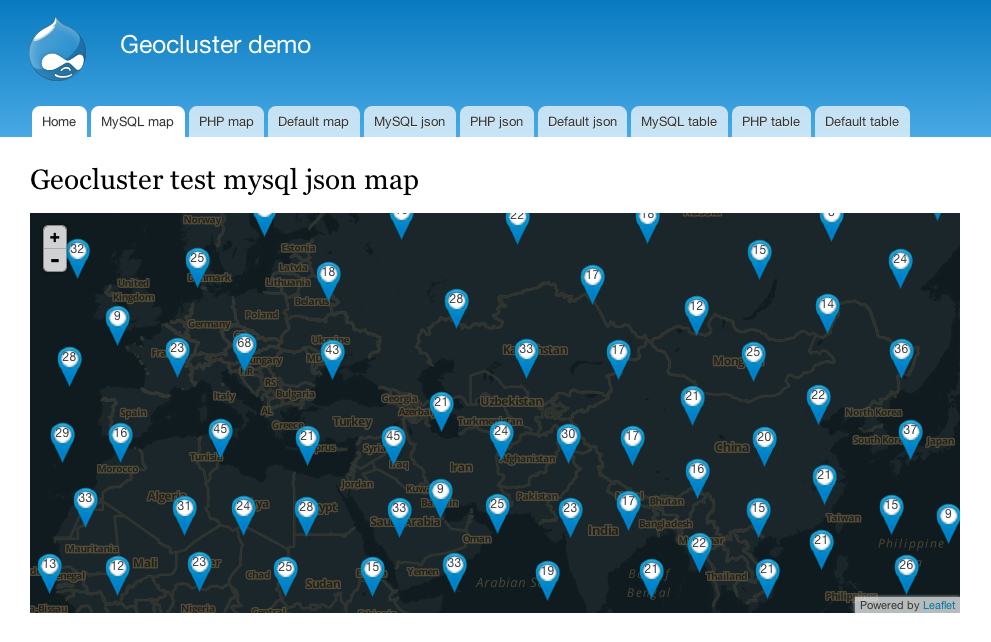
\includegraphics[width=1\textwidth]{figures/geocluster_demo_site.png}
    \caption{Screenshot of a Geocluster Demo installation. The active tab shows a map that uses MySQL-based clustering.}
    \label{fig:geocluster-demo-site}
  \end{center}
\end{figure}

\section{GeoRecruiter}
\label{chapter:use-case-georecruiter}

A practical use case for server-side geo clustering has been implemented for the Recruiter job board solution which has been introduced in chapter \ref{chapter:objective-use-cases}. It supports spatial search capabilities of the Recruiter distribution by visualizing a large amount of job offers on e-recruitment websites. GeoRecruiter allows to visualize several thousands of available jobs on an interactive map for large-scale e-recruitment websites. The Geocluster Solr module has been designed and used to provide the clustering capabilities needed by GeoRecruiter. The Solr-based aggregation integrates well with the architecture of the Recruiter distribution and is designed for scalability up to 1,000,000 indexed jobs as evaluated in chapter \ref{chapter:performance}. The prototype being discussed in the following chapter has been developed based on a copy of the Drupaljobs website\footnote{\url{http://drupaljobs.epiqo.com}}.

Drupaljobs is provided by epiqo as a show case for the Recruiter distribution. Its base features allow to create and search for job offers by companies as well as resumes of registered applicants on the e-recruitment platform. Figure \ref{fig:recruiter-job-search} depicts a screenshot of the heart of a Recruiter installation: the job search. The numbers on the figure indicate the main parts of such a page:

\begin{enumerate}

\item [(1)] A \textbf{search bar} above the content region.
\item [(2)] \textbf{Facetted filters} in the left sidebar.
\item [(3)] The \textbf{search results} as job teasers matching the search and filters.

\end{enumerate}

For scalability reasons, the job search functionality of Recruiter is based on Apache Solr using the Search API module which have been introduced in chapter \ref{chapter:data-storage}. The concept of using facetted filters, allows the site visitor to narrow down the result set by applying filters based on properties of the result set. The screenshot from figure \ref{fig:recruiter-job-search} displays filter facets based on \textit{organization}, \textit{fields of study} and \textit{occupational fields}. Every filter item indicates the number of results to be expected when using this particular filter. 

\begin{figure}[h]
  \begin{center}
    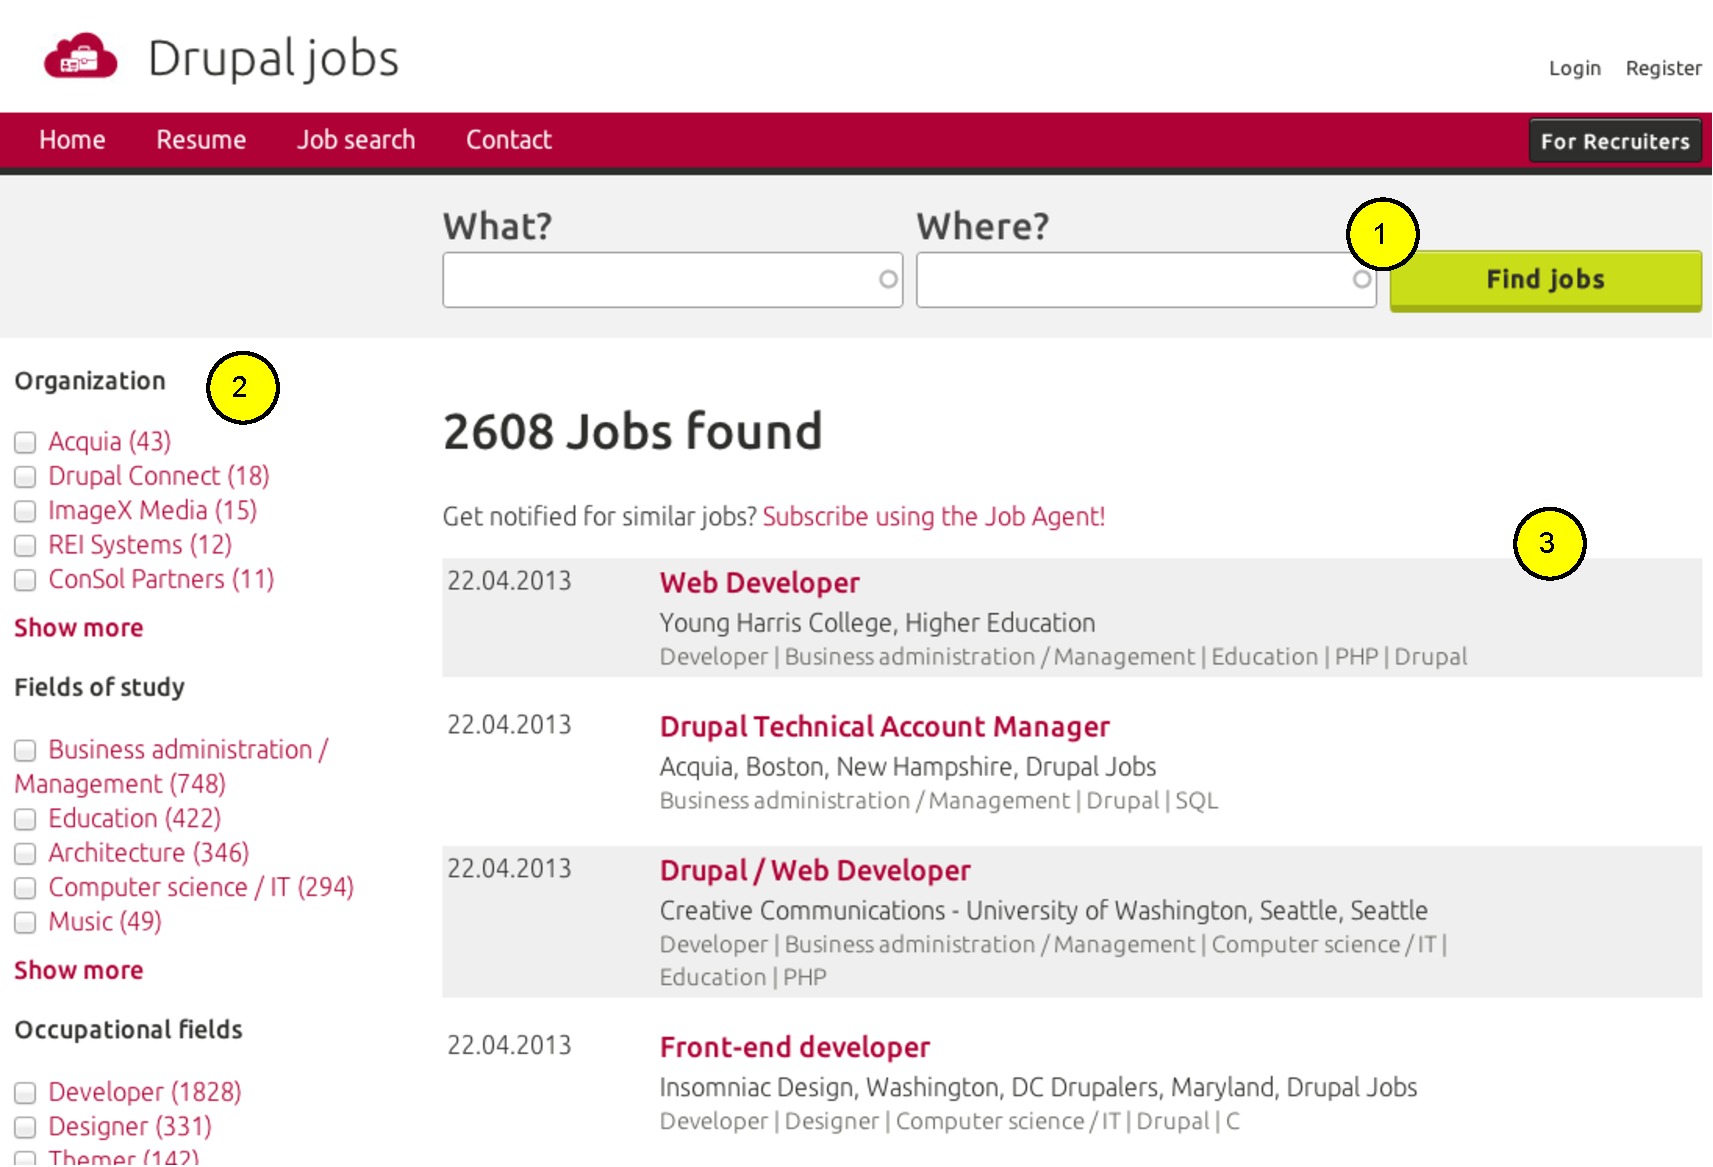
\includegraphics[width=1\textwidth]{figures/recruiter_job_search.pdf}
    \caption{Screenshot of a job search on Drupaljobs including indicators: (1) search bar, (2) facetted filters and (3) search results.}
    \label{fig:recruiter-job-search}
  \end{center}
\end{figure}

The GeoRecruiter use case consists of several geo-related additions to the Recruiter distribution. As previously stated, the customizations have been prototyped using a Drupaljobs test installation.

\begin{itemize}

\item \textbf{Add geospatial data}: The data model for posting job offers of the Recruiter distribution has been extended to support the annotation of a geospatial location as the \textit{place} property. In particular, a Geofield was added to the job node content types.

\item \textbf{Import test data}: Two sets of real-world geospatial test data have been prepared for the Drupaljobs test site. A set of 10,000 world-wide cities was created based on a dataset from GeoNames.org\footnote{\url{http://download.geonames.org/export/dump/cities1000.zip}}. Another set of 100,000 of U.S.-specific landmarks is based on a dataset from the U.S. Board on Geographic Names\footnote{\url{http://geonames.usgs.gov/docs/stategaz/NationalFile_20130404.zip}}. The kind of data isn't necessarily related to but will be mapped to job offers. This approach was taken due to the lack of a geospatially annotated datasets of job offers being available for testing purposes. Next, the test data was cleaned from errors and imported into the adapted Drupaljobs test installation. The import process was facilitated by using the Feeds module\footnote{\url{http://drupal.org/project/feeds}} which allows to import data into a Drupal site from external data sources like RSS feeds or in this particular case: CSV files.

\item \textbf{Configure Geocluster Solr}: The server-side clustering component explained in \ref{chapter:architecture-implementation} has been installed on the Drupaljobs test instance. The job search has been configured for clustering based on Apache Solr and Search API. Finally, a map visualizes the clustered job search results using Views GeoJSON and Leaflet. In order to enhance the representation of clusters and to experiment with interaction, the CSS styles of the client-side clustering library Leaflet.markercluster have been adapted and extended with additional colors for large clusters.

\item \textbf{Compare with client-side clustering}: In order to measure the effectiveness of the server-side clustering approach, a client-side clustering solution has been implemented for Drupaljobs as well. The client-side clustered map is based on a blog post by Ian Whitcomb of LevelTen~\cite{blog:leaflet-made-to-order}. For querying such a large dataset, he recommends circumnavigating the Views module and directly querying the database. The client-side clustering and visualization is again realized by the Leaflet.markercluster.

\end{itemize}

The resulting prototype allowed to experiment with the server-side clustering solution in a realistic environment, draw conclusions on effectiveness of clustering algorithm and the visualization component being used. A visualization of a map within the Drupaljobs test installation is provided in figure \ref{fig:drupaljobs-geocluster-solr}.

\begin{figure}[h]
  \begin{center}
    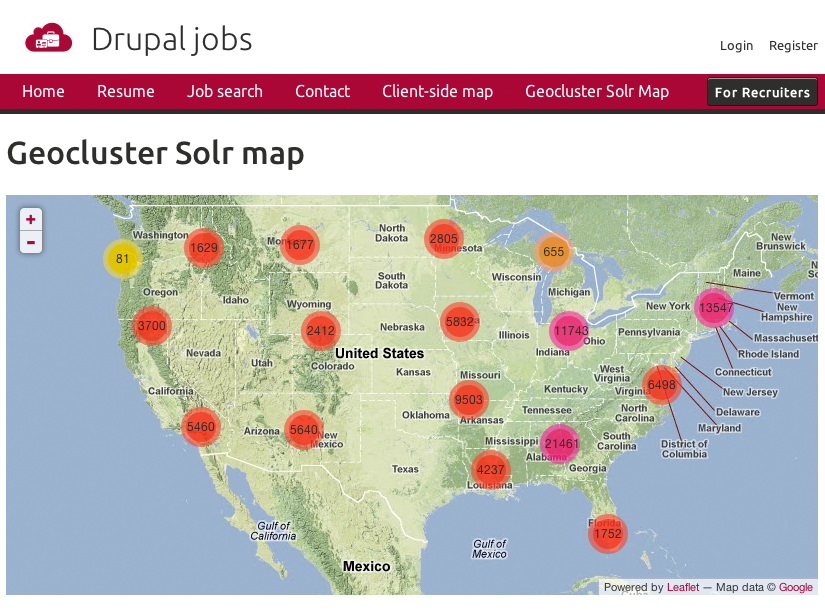
\includegraphics[width=1\textwidth]{figures/drupaljobs_geocluster_solr.png}
    \caption{Screenshot of map that visualized job search results on a map using Solr-based clustering on a Drupaljobs test installation.}
    \label{fig:drupaljobs-geocluster-solr}
  \end{center}
\end{figure}


Besides the clustering functionality, GeoRecruiter will support location-based search. This allows the user to search for jobs within the surroundings of a desired region by applying a proximity filter. The Search API Location module is currently being refactored\footnote{\url{http://drupal.org/node/1798168}} in order to provide a solid foundation for such spatial queries using Solr and the Search API module suite.










%
% conclusions
%

\chapter{Conclusions \& outlook}
\label{chapter:conclusions-outlook}

\section{Performance evaluation}
\label{chapter:performance}

Performant real-time clustering is the main objective of this thesis as formulated in chapter \ref{chapter:objective-performance}. As a requirement, the algorithm should cluster in real-time to support dynamic queries and cluster up to 1,000,000 items within less than one second.

The configuration of the demo use case implementation described in chapter \ref{chapter:use-case-demo} was used to do automated performance testing of the different clustering algorithms. A \textit{Bash}\footnote{\url{http://en.wikipedia.org/wiki/Bash\_(Unix\_shell)}} script was created to test the performance of the clustering algorithm based against an incrementing number of items.

\begin{figure}[h]
  \begin{center}
    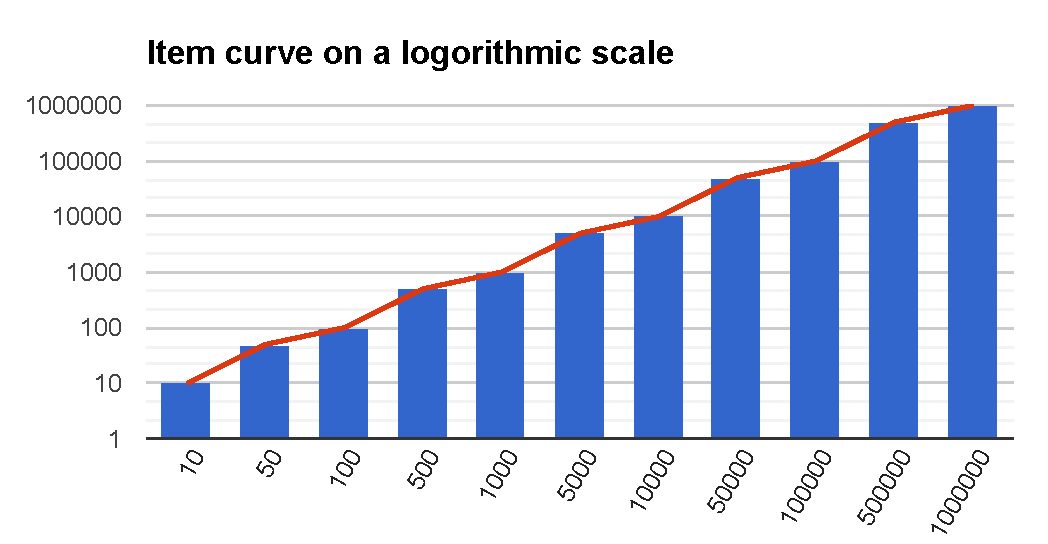
\includegraphics[width=0.8\textwidth]{figures/performance_items.pdf}
    \caption{Item curve on a logorithmic scale.}
    \label{fig:performance-items}
  \end{center}
\end{figure}

The script exponentially increases items to test the clustering performance from a base 10 up to 1,000,000 items. Between every two steps of the exponential function, an intermediary step of the half of the two steps will be inserted. While the exponential mean value for example between 100 and 1000 items would be 316.2, this approach inserts 500 to improve readability of the results for humans. The resulting curve of items tested is visualized in figure \ref{fig:performance-items}.

The \textit{ab} command of the ApacheBench\footnote{\url{http://en.wikipedia.org/wiki/ApacheBench}} is used to sequentially repeat the same requests and calculate a mean response time value. Hereby the script tries to circumvent variations caused by external factors as the server hardware and operating system.

The results of the performance benchmark have been extracted and aggregated into a chart as show in figure \ref{fig:algorithm-performance}. It is clearly shown that that the three implemented algorithms perform very differently. Each algorithm scales up to a certain number of items, while beyond this threshold, performance decreases significantly. The PHP-based clustering algorithm is very limited in such that requests for up to 1,000 clustered items can be completed within one second. The MySQL-based clustering approach scales much better but requests get slow beyond 100,000 items. The most performant algorithm implementation is the Solr-based one that server 1,000,000 items still in a reasonable amount of time. 

\begin{figure}[h]
  \begin{center}
    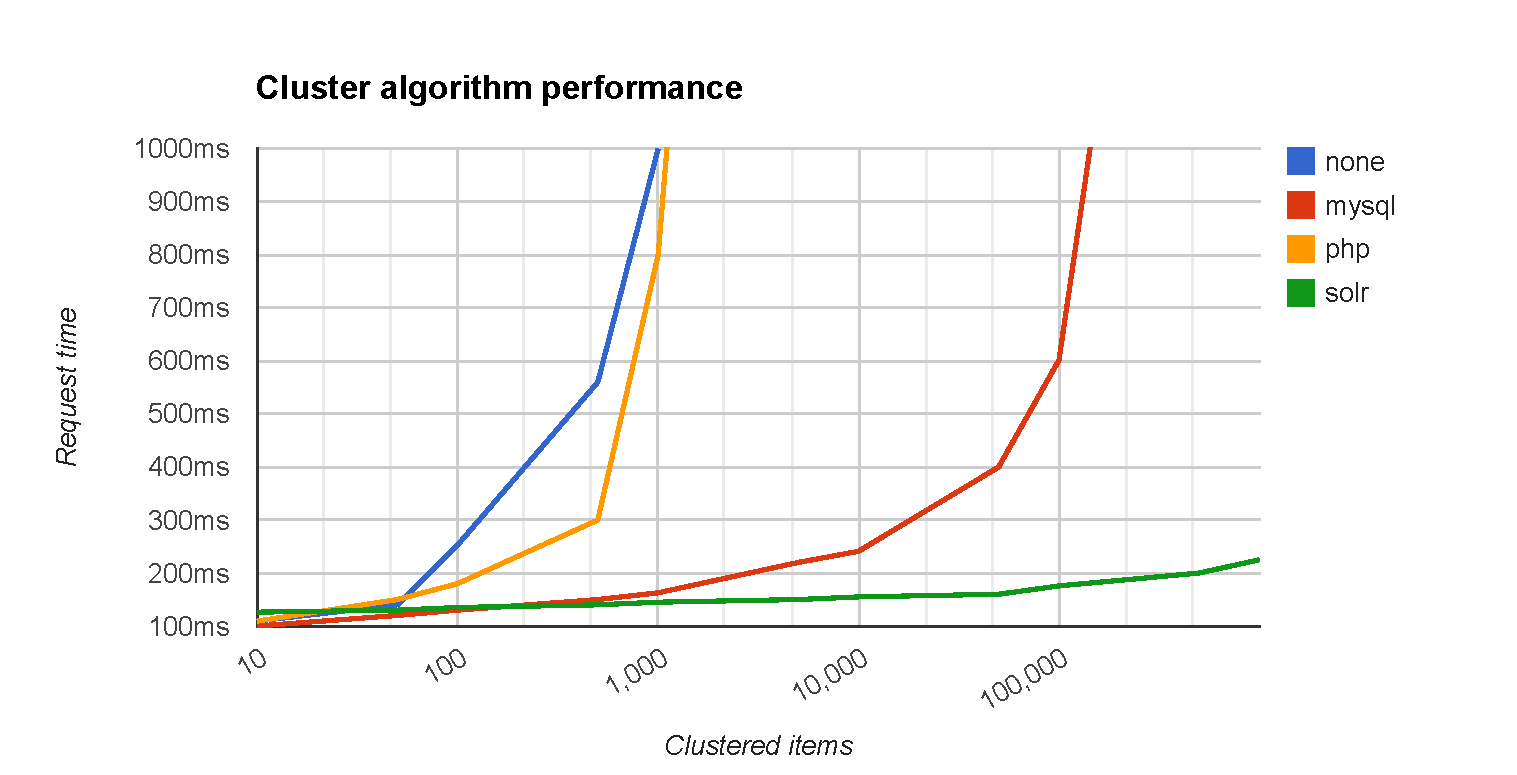
\includegraphics[width=1.2\textwidth]{figures/geocluster_algorithm_performance.pdf}
    \caption{Geocluster performance in milliseconds per algorithm and number of items.}
    \label{fig:algorithm-performance}
  \end{center}
\end{figure}

A deeper analysis of the PHP-based algorithm clearly shows that the most time-consuming part of the algorithm is creating the clusters based on Geohash. As all unclustered items need to processed after executing the database query have to be processed, this part takes the most time. In an example based on a query with 9270 items, the entire roundtrip between client and server takes 26.71 seconds. Querying the items just took 100ms. With 24.32 seconds, the Geohash-based pre-clustering consumes the major part of the execution time. For the same amount of items, a request using the MySQL-based algorithm was completed within 194 ms. In this case, the query was completed after 80 ms and the while clustering process was finished 8 ms seconds later. The remainder of the processing time was consumed by Drupal performing non-clustering related processing before and at the end of the request. This example shows, how shifting the main clustering task into the database can increase performance for a certain range of number of items. As stated before, when approaching 100,000 items the MySQL-based algorithm is getting significantly slower, as the query itself takes longer.

Given the numbers, the performance criterion of this thesis could be fulfilled. While the PHP-based implementation isn't really usable, MySQL-based and Solr-based clustering can be used to create performant, interactive maps with Drupal for item sets up to at least 1,000,000 items. While we know that MySQL-based clustering only scales up to 100,000 items, the threshold for Solr-based clustering wasn't determined as tests were limited up to 1,000,000 items. It is expected that there is room for improvements and optimizations for all of the algorithms.

Another performance-related aspect is cachability of responses and results. Apache Solr and Drupal itself already incorporate various caching layers. Caching clustered results for the server-side clustering solution mainly depends on the parameters of the Bounding Box strategy. As currently, every minor change to the bounding box will issue a different request to the server, these can't be cached efficiently. A possible solution discussed\footnote{\url{http://drupal.org/node/1868982}} is to define granular steps for the bounding box in order to produce repeating requests that can be cached.  

\section{Further evaluation \& conclusions}

The second objective on integration and extensibility defined in chapter \ref{chapter:objective-integration} has been fulfilled by the Geocluster module as it integrates with Views, Views GeoJSON and other Drupal mapping modules. In addition, the implementation of the clustering algorithm can be extended using plugins as explained in chapter \ref{chapter:impl-alg}. Geocluster was also released under the GPL license as required by objective \ref{chapter:open-source}. With regards to objective \ref{chapter:objective-use-cases}, a demo use case has been implemented that show cases all the functionality needed. The actual GeoRecruiter use case hasn't been implemented, but as stated in \ref{chapter:use-case-georecruiter}, the groundwork has been established in order to do so. Finally, main usability concerns have been realized with the Geocluster Visualization component.

While most objectives have been reached, there are still many parts of the Geocluster implementation that can be improved upon:

\begin{itemize}

\item \textbf{Cluster sizes}: The current implementation doesn't respect the size of a cluster. As naturally, a cluster with more items can be visualized larger than smaller clusters, the algorithm could be improved for growing clusters by their size. The bigger size of a cluster would therefore reduce the distance to its neighbor clusters, potentially merging additional neighbors into it. Andrew Betts describes a similar approach under the term \textit{``Grid based viral growth argorithm''}\footnote{\url{http://web.archive.org/web/20071121140547/http://trib.tv/tech/clustering-points-on-a-google-map/}}.

\item \textbf{Cluster centers}: While the PHP- and MySQL-based algorithm provide means of calculating a centroid as the center of a cluster, the Solr-based clustering algorithm is limited in this regards. Solr doesn't seem to provide the same functionality to calculate the mean value for a field using the grouping function, as the MySQL-based algorithm leverages the $AVG$ function for latitude and longitude. Potentially, the stats component\footnote{\url{http://wiki.apache.org/solr/StatsComponent}} could be used for calculating the centroid of cluster items within the Solr-based algorithm.

\item \textbf{Processing clustered results}: The way that the Drupal mapping stack integrates with the Views module isn't designed for processing clustered results. The current implementation of Geocluster performs various workarounds in order to inject clustered results into the process. Especially for the Solr-based implementation this leads to code-duplication because in the standard case results are processed as arrays while in the other case, results need to be PHP objects. If possible, a cleaner way of integrating clustering with the related modules is desirable.   

\item \textbf{Improve client-side handling and visualization}: The current implementation for visualizing clustered results is very basic. A relative sizing of cluster items according to their clusters is needed and should also be supported by the algorithm as stated before. In addition, it would be good to have be a clean way to configre the how data for clustered results should be displayed and integrate it with how non-clustered data is represented. For low zoom levels, the roundtrip to the server for fetching a separate clustered result on every bounding box change can be an overhead. Christopher Calid\footnote{\url{http://drupal.org/user/210499}} proposed a way of ``Progressively enhance server-side with client-side clustering''\footnote{\url{http://drupal.org/node/1914704}}. The intention is to transition from server-side clustering higher zoom levels to client-side clustering for lower zoom levels.

\end{itemize}

Writing this thesis and implementing Geocluster was basically a process of over one year. Before starting the thesis, I conducted a research project named AustroFeedr\footnote{\url{http://www.austrofeedr.at/}} on real-time processing technologies for aggregating, processing and visualizing data with Drupal. One main aspect of AustroFeedr was a Drupal-based visualization component using OpenLayers maps. After I had completed AustroFeedr by the end of 2011, I researched Drupal and mapping related topics for writing this master thesis in Software Engineering \& Internet Computing at Technical University Vienna.

The topic server-side clustering for Drupal was decided upon thanks to recommendation by Th\'eodore Biadala\footnote{\url{http://drupal.org/user/598310}}, an active JavaScript and maps contributor in the Drupal community who I met at the Frontend United conference in Amsterdam, April 20-22. After doing some initial research and prototyping, I organized a mapping sprint at Drupal Developer Days Barclona\footnote{\url{http://groups.drupal.org/node/234168}}. This is where Nick Veenhof\footnote{\url{http://drupal.org/user/122682}}, active Apache Solr contributor within the Drupal community, came up with the idea of researching Geohash for realizing an efficient clustering algorithm.

It took until September 2012, when I implemented a first prototype of the PHP-based clustering algorithm and figured out basic integration needs for to make the clustering task work with Drupal. From then, several iterations and alpha releases of Geocluster led to completing MySQL and Solr-based clustering by the end of 2012. As by finishing this thesis in March 2013, performance tests have been concluded for Geocluster and a first beta release has been published.

There has already been some positive feedback from people interested in using Geocluster as a drop-in solution to create scalable maps using server-side clustering. On the other hand, I have to admit that integration clustering into a complex stack such as the Drupal mapping stack has its advantages and disadvantages. Geocluster does a decent job at clustering data server-side, but the tight integration into the Drupal stack also comes at the cost of overhead and complex integration code. Given the expertise in writing code, it can make sense to create a custom server-side clustering solution for a specific purpose without depending on a number of separate modules. Still, the generic approach has the benefit of others potentially being able to use the Geocluster module. Writing this thesis was both challenging and fun. Working on something and being able to share it with the Drupal community, a steadily growing team of contributors of Free and Open Source software, has been a rewarding experience and a solid source of motivation. 

\section{Future work}

Direct community feedback and indirect indicators like the project usage statistics will show if and how the Geocluster module is used by others. As stated before, there are many implementation details that can be enhanced. At epiqo, we are planning to incorporate Geocluster for location-based searches of large-scale job portals based on the Recruiter distribution as stated in chapter \ref{chapter:use-case-georecruiter}. 

Thanks to a scholarship by the Drupal association, I will be able to attend DrupalCon Portland\footnote{\url{http://portland2013.drupal.org/}}. Together with other Drupal mapping contributors, we have proposed a panel discussion\footnote{\url{http://portland2013.drupal.org/session/should-have-made-left-turn-albuquerque-panel-discussion-challenges-buildingincorporating}} which would be a great opportunity to discuss server-side clustering as one strategy for creating scalable, interactive maps with Drupal.



\newpage

\appendix
\chapter{Acronyms}

\begin{acronym}
\acro{AJAX}{Asynchronous JavaScript + XML}
\acro{API}{Application Programming Interface}
\acro{BBOX}{Bounding Box}
\acro{CMS}{Content Management System}
\acro{DBSCAN}{Density-based spatial clustering of applications with noise}
\acro{GNU}{GNU's Not Unix}
\acro{GeoJSON}{JSON for geographic data structures}
\acro{GIS}{Geographic Information System}
\acro{HTML}{HyperText Markup Language}
\acro{HTTP}{HyperText Transfer Protocol}
\acro{IDE}{Integrated Development Environment}
\acro{IT}{Information Technology}
\acro{JSON}{JavaScript Object Notation}
\acro{OASIS}{Organization for the Advancement of Structured Information Standards}
\acro{PHP}{PHP: Hypertext Preprocessor}
\acro{REST}{Representational State Transfer}
\acro{RSS}{Really Simple Syndication}
\acro{SOM}{Self-organizing maps}
\acro{STING}{Statistical Information Grid}
\acro{TMS}{Tile Map Service}
\acro{UDDI}{Universal Description, Discovery and Integration}
\acro{UI}{User Interface}
\acro{URI}{Uniform Resource Identifier}
\acro{URL}{Uniform Resource Locator}
\acro{W3C}{World Wide Web Consortium}
\acro{WMS}{Web Map Service}
\end{acronym}

\chapter{Index}
\listoffigures
\listoftables
\lstlistoflistings

%%%%%%%%%%%%%%%%%%%%%%%%%%%%%%%%%%%%%%%%
% PUT APPENDIX, BIBLIOGRAPHY, ... HERE %
%%%%%%%%%%%%%%%%%%%%%%%%%%%%%%%%%%%%%%%%

\bibliographystyle{alpha}
%\bibliographystyle{alpha}
\bibliography{bib/references}

\end{document}

%%% Local Variables:
%%% TeX-PDF-mode: t
%%% TeX-debug-bad-boxes: t
%%% TeX-master: t
%%% TeX-parse-self: t
%%% TeX-auto-save: t
%%% reftex-plug-into-AUCTeX: t
%%% End: